\clearpage
\setcounter{page}{1}

\section{Tutorial membuat aplikasi oracle apex}
\paragraph{}
    Sebelum itu mari kita siapkan data mentahan yang kita ambil dari materi database semester 1 di bab 3. Lalu analisis data tersebut, dan lakukanlah normalisasi. Adapun tabel yang didapat setelah melakukan normalisasi adalah Tabel Mahasiswa, Dosen, Kuliah, Nilai, dan Jadwal. 
\begin{enumerate}
    \item Lakukan normalisasi pada tabel mahasiswa menggunakan text editor atau spreadsheet, disini saya menggunakan WPS Spreadsheet. Adapun field dalam tabel tersebut adalah NIM, Nama Mahasiswa, Alamat Mahasiswa, dan Tanggal Lahir.
    \begin{figure}[ht]
    \centerline{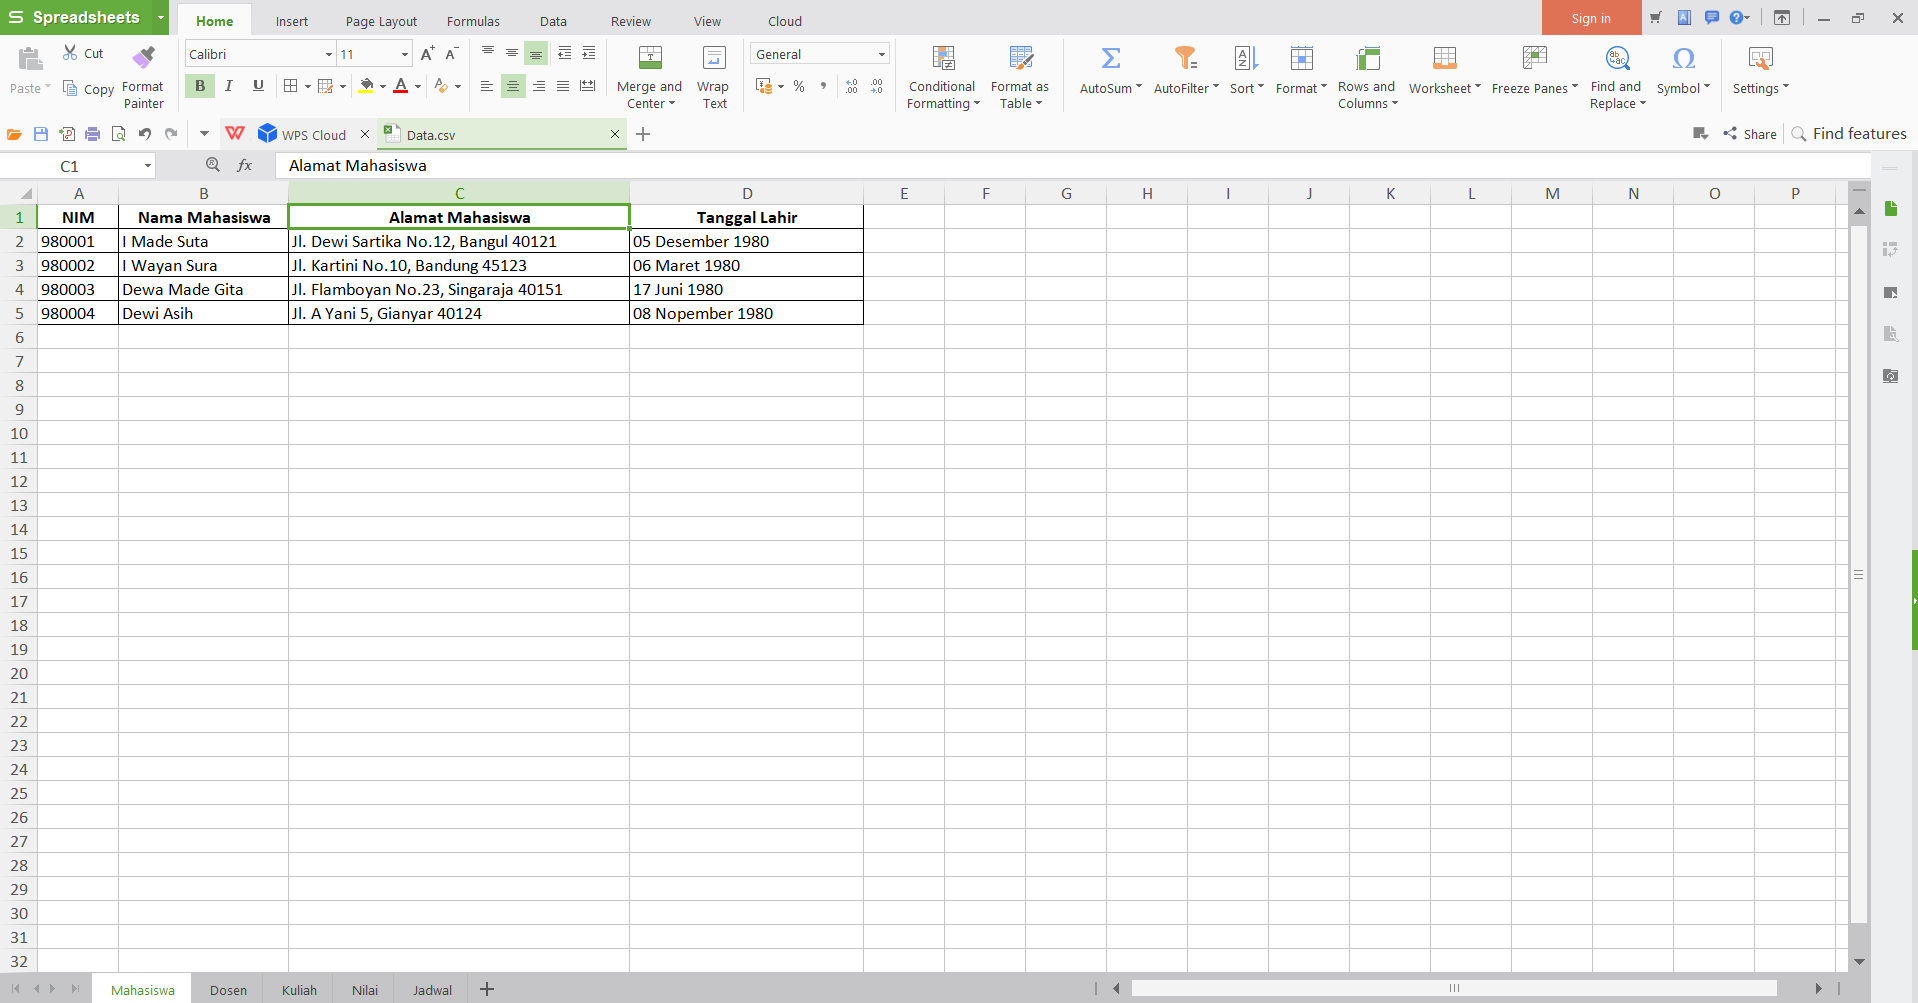
\includegraphics[width=10cm]{Figures/Mahasiswa.PNG}}
    \end{figure}
    \item Lakukan normalisasi pada tabel dosen menggunakan text editor atau spreadsheet, disini saya menggunakan WPS Spreadsheet. Adapun field dalam tabel tersebut adalah NIK, Nama Dosen, Alamat Dosen.
    \begin{figure}[ht]
    \centerline{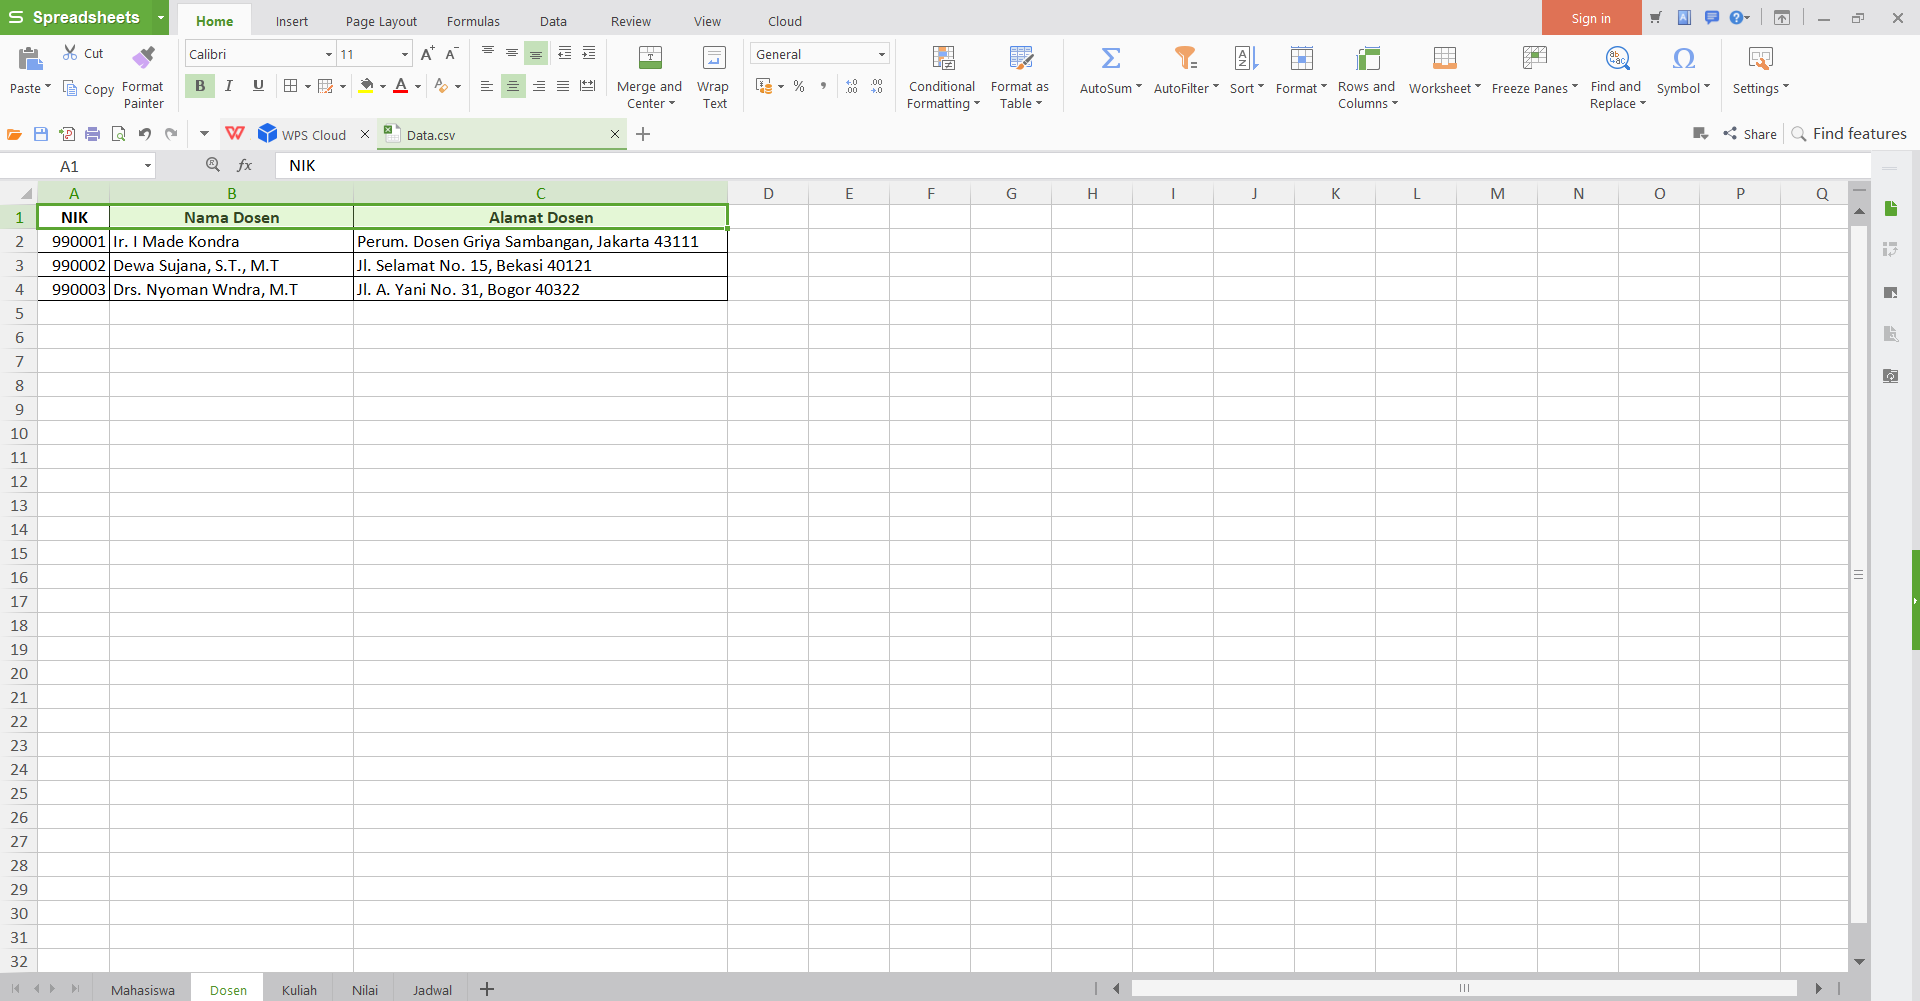
\includegraphics[width=10cm]{Figures/Dosen.PNG}}
    \end{figure}
    \item Lakukan normalisasi pada tabel nilai menggunakan text editor atau spreadsheet, disini saya menggunakan WPS Spreadsheet. Adapun atribut dalam tabel tersebut adalah Indeks Nilai sedangkan NIM merupakan foreign key dari tabel Mahasiswa dan Kode merupakan foreign key dari tabel Kuliah.
    \begin{figure}[ht]
    \centerline{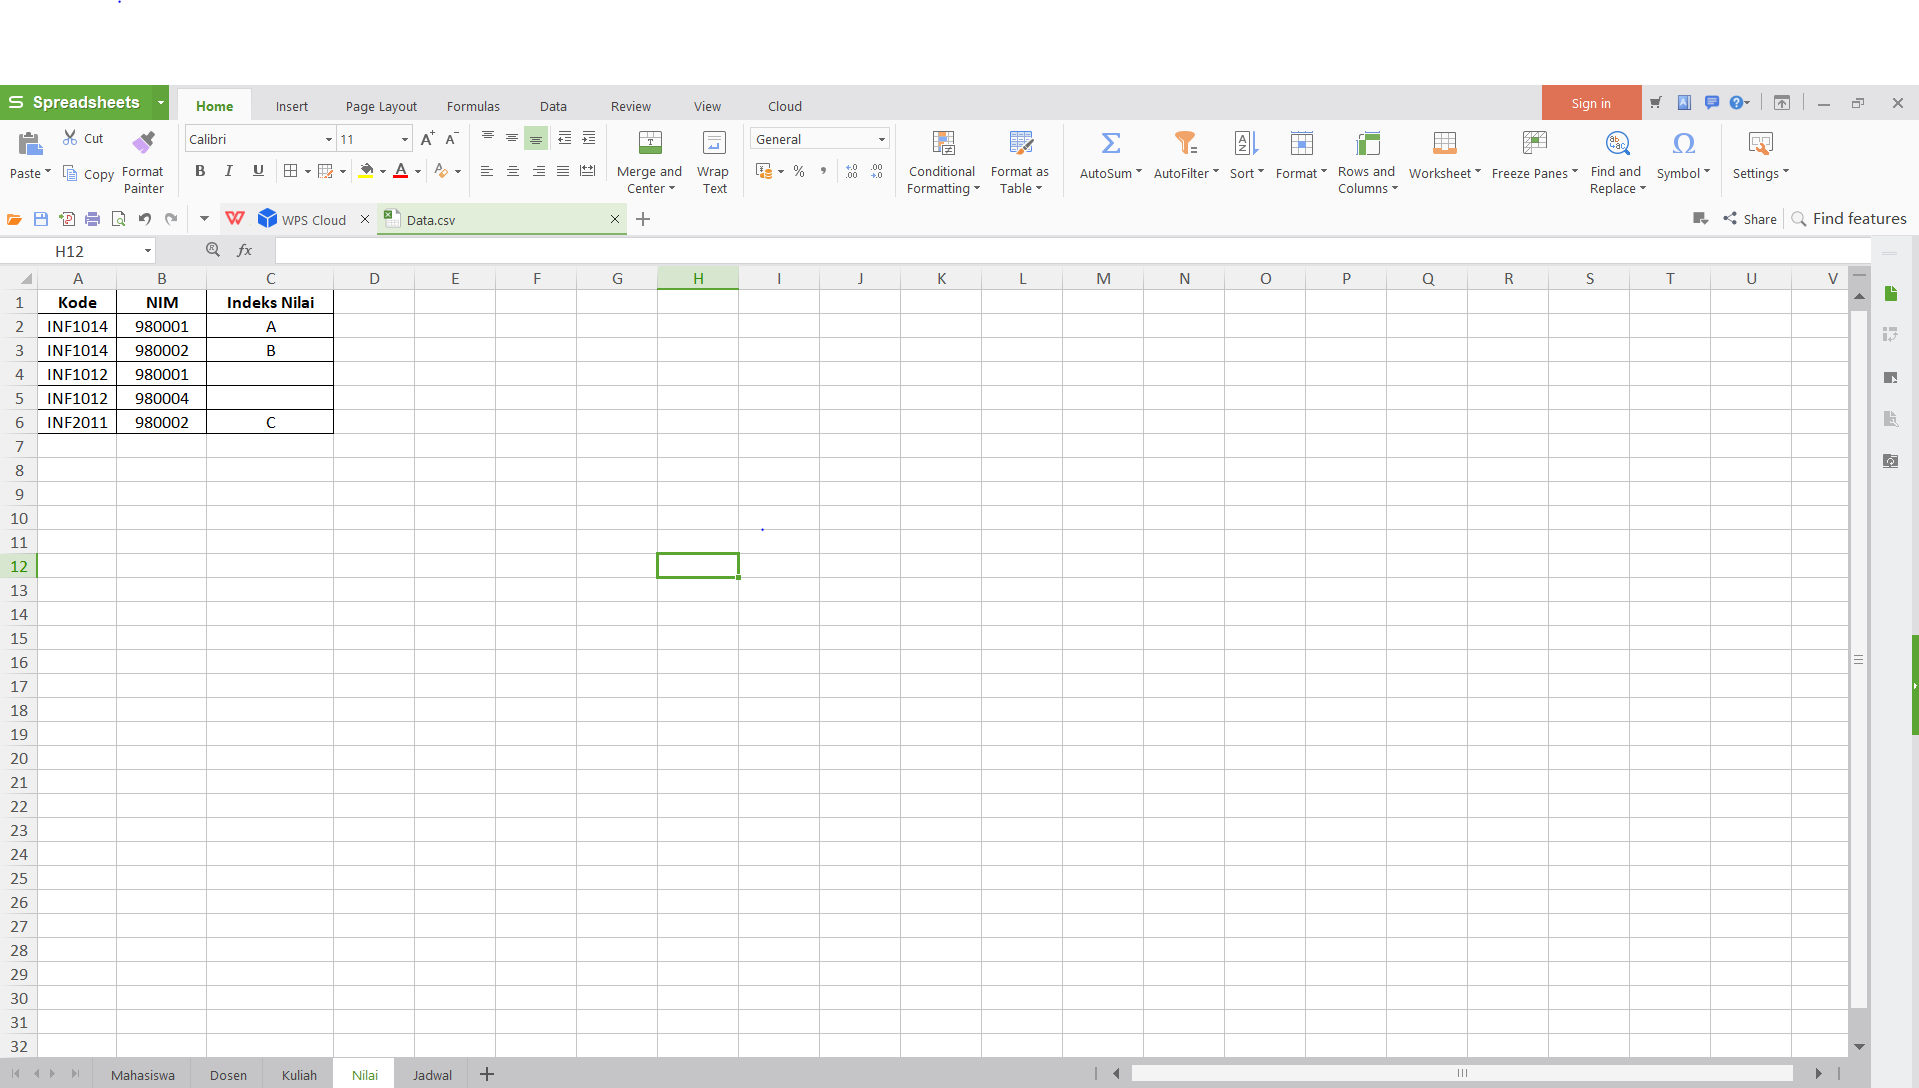
\includegraphics[width=10cm]{Figures/Nilai.PNG}}
    \end{figure}
    \item Lakukan normalisasi pada tabel kuliah menggunakan text editor atau spreadsheet, disini saya menggunakan WPS Spreadsheet. Adapun atribut dalam tabel tersebut adalah SKS, Semester, Kode.
    \begin{figure}[ht]
    \centerline{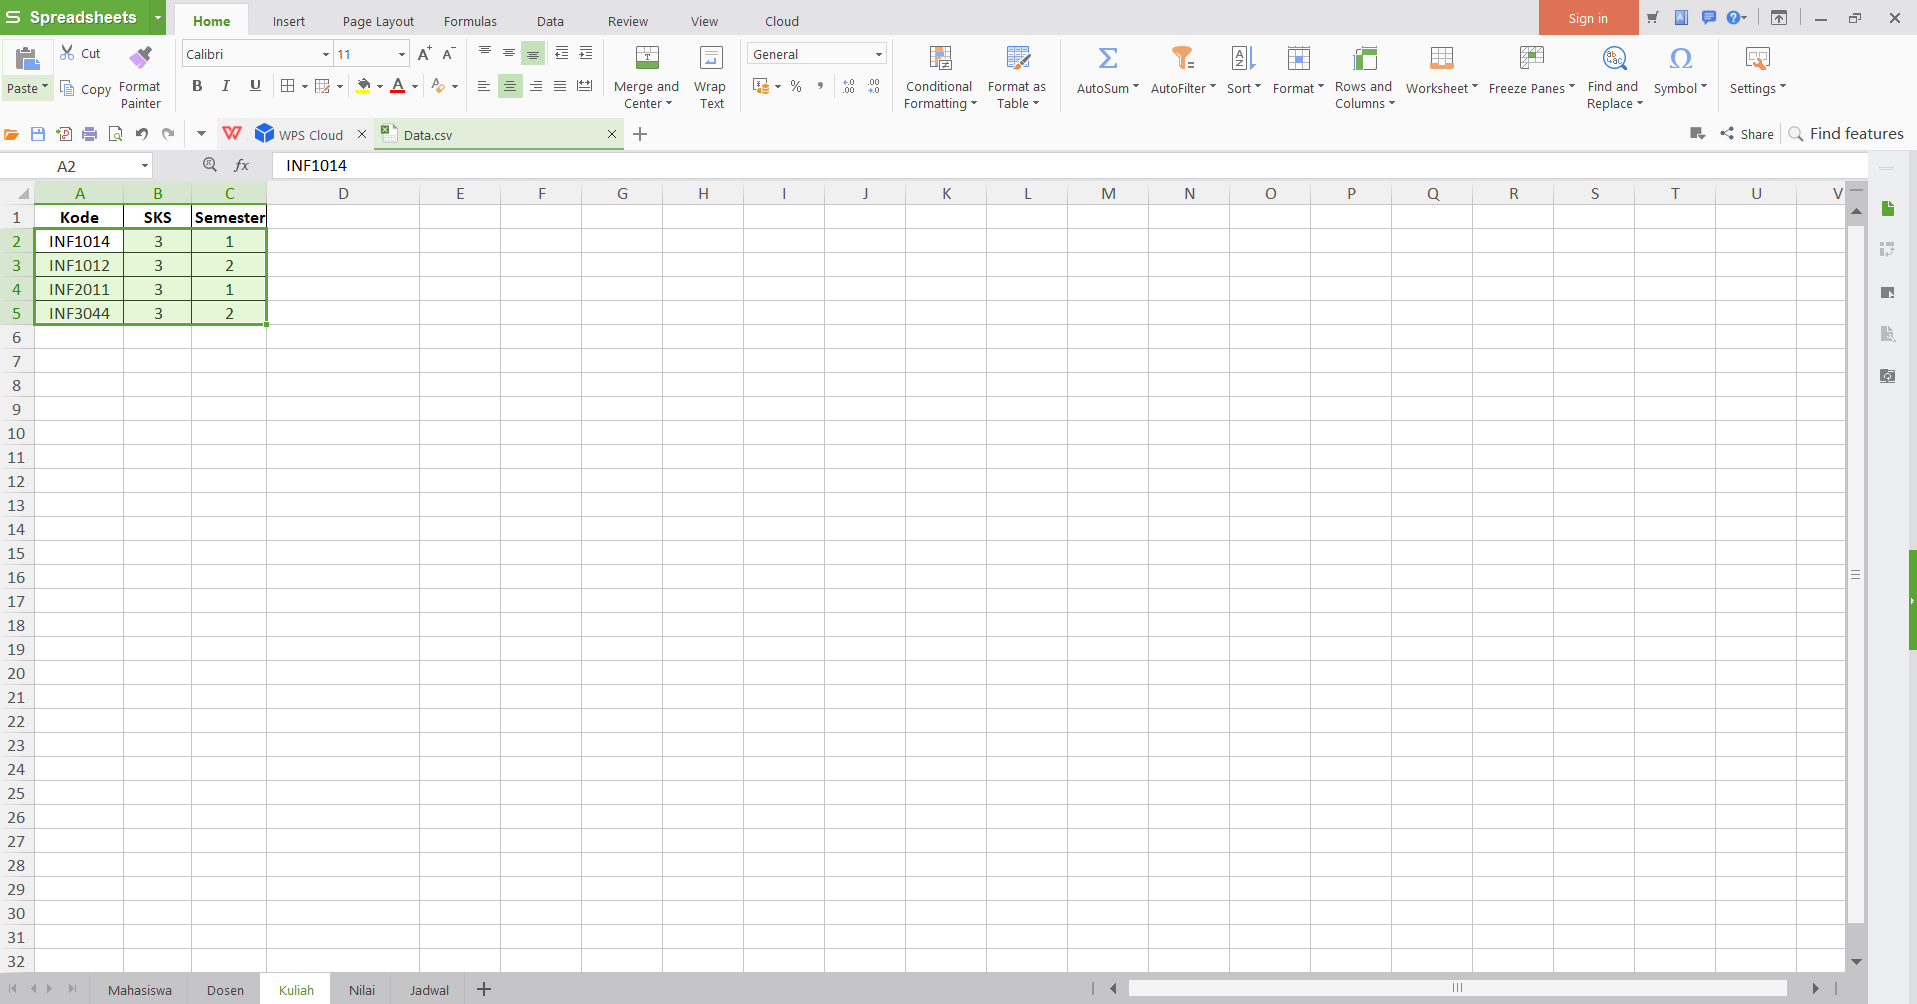
\includegraphics[width=10cm]{Figures/Kuliah.PNG}}
    \end{figure}
     \item Lakukan normalisasi pada tabel kuliah menggunakan text editor atau spreadsheet, disini saya menggunakan WPS Spreadsheet. Adapun atribut dalam tabel tempat dan waktu sedangkan kode merupakan foreign key dari tabel kuliah dan Nik merupakan foreign key dari tabel dosen.
    \begin{figure}[ht]
    \centerline{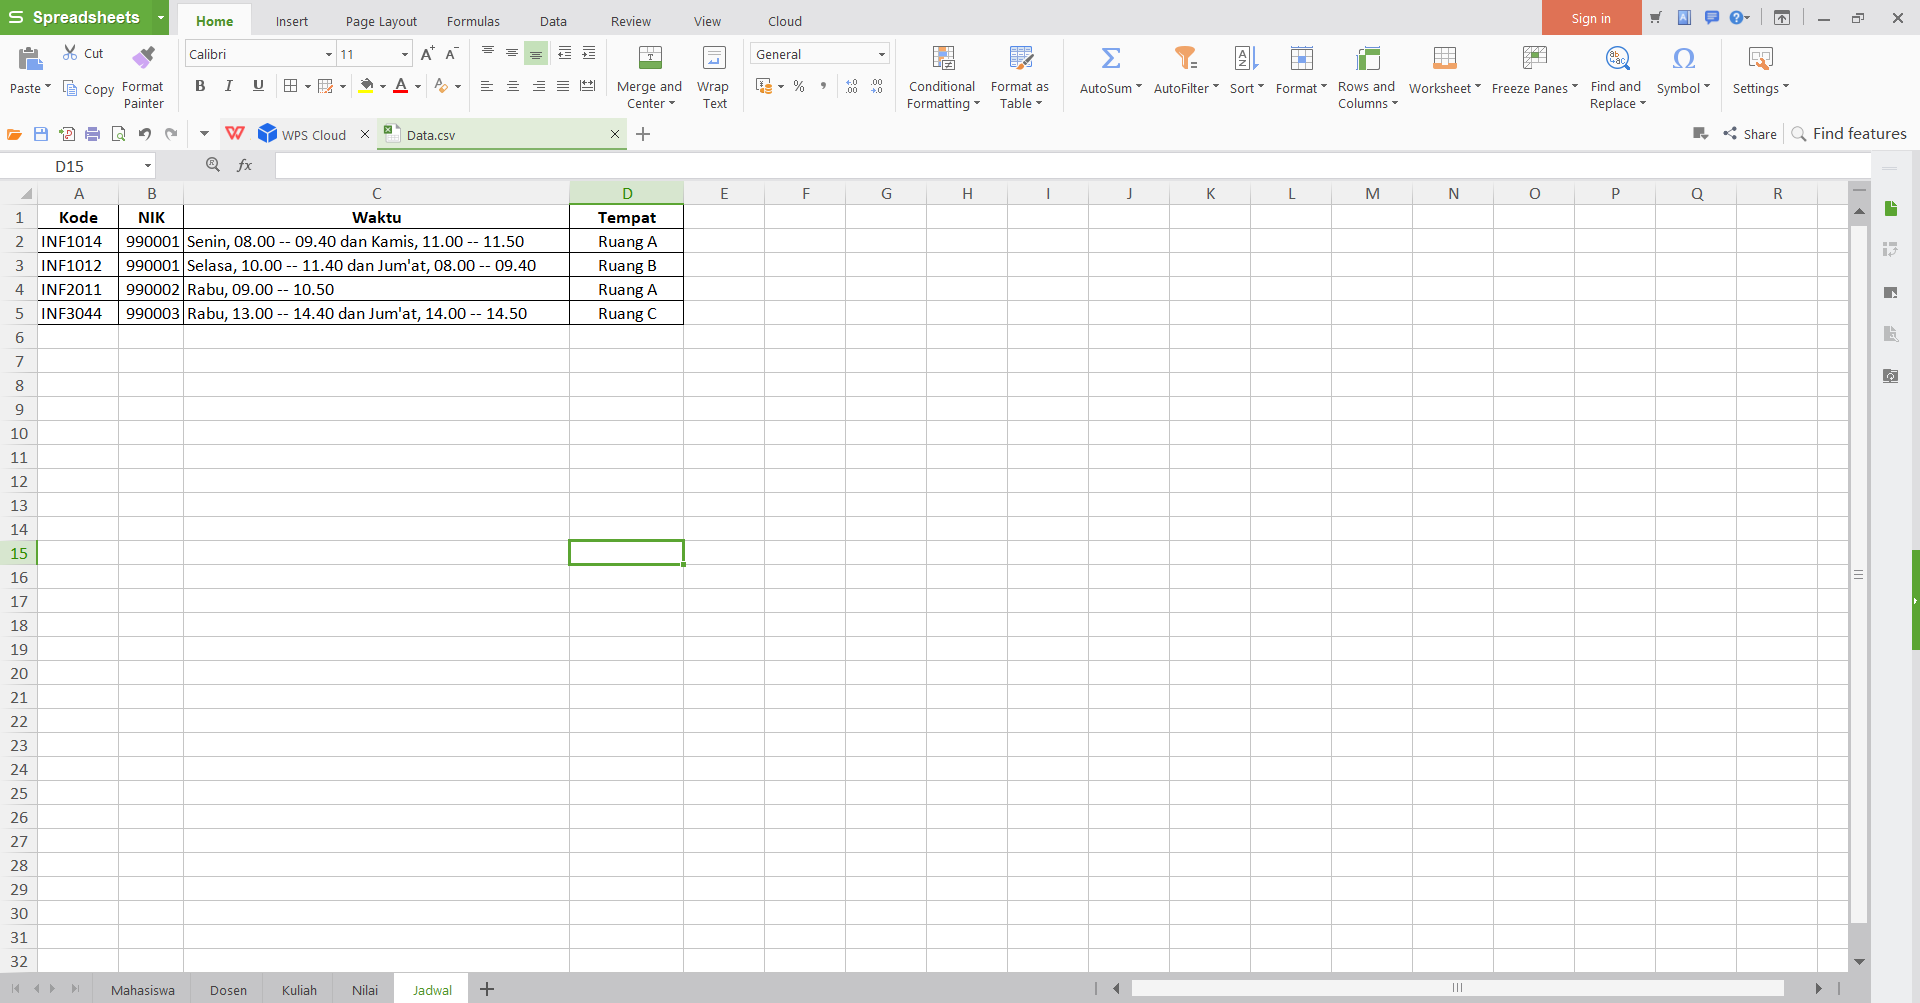
\includegraphics[width=10cm]{Figures/Jadwal.PNG}}
    \end{figure}
    \item Buka oracle apex online \textit{oracle.apex.com}. Untuk yang belum memiliki akun anda bisa memilih get started for free dan bagi anda yang sudah memiliki akun anda bisa langsung sign in.
        \begin{figure}[h]
        \centerline{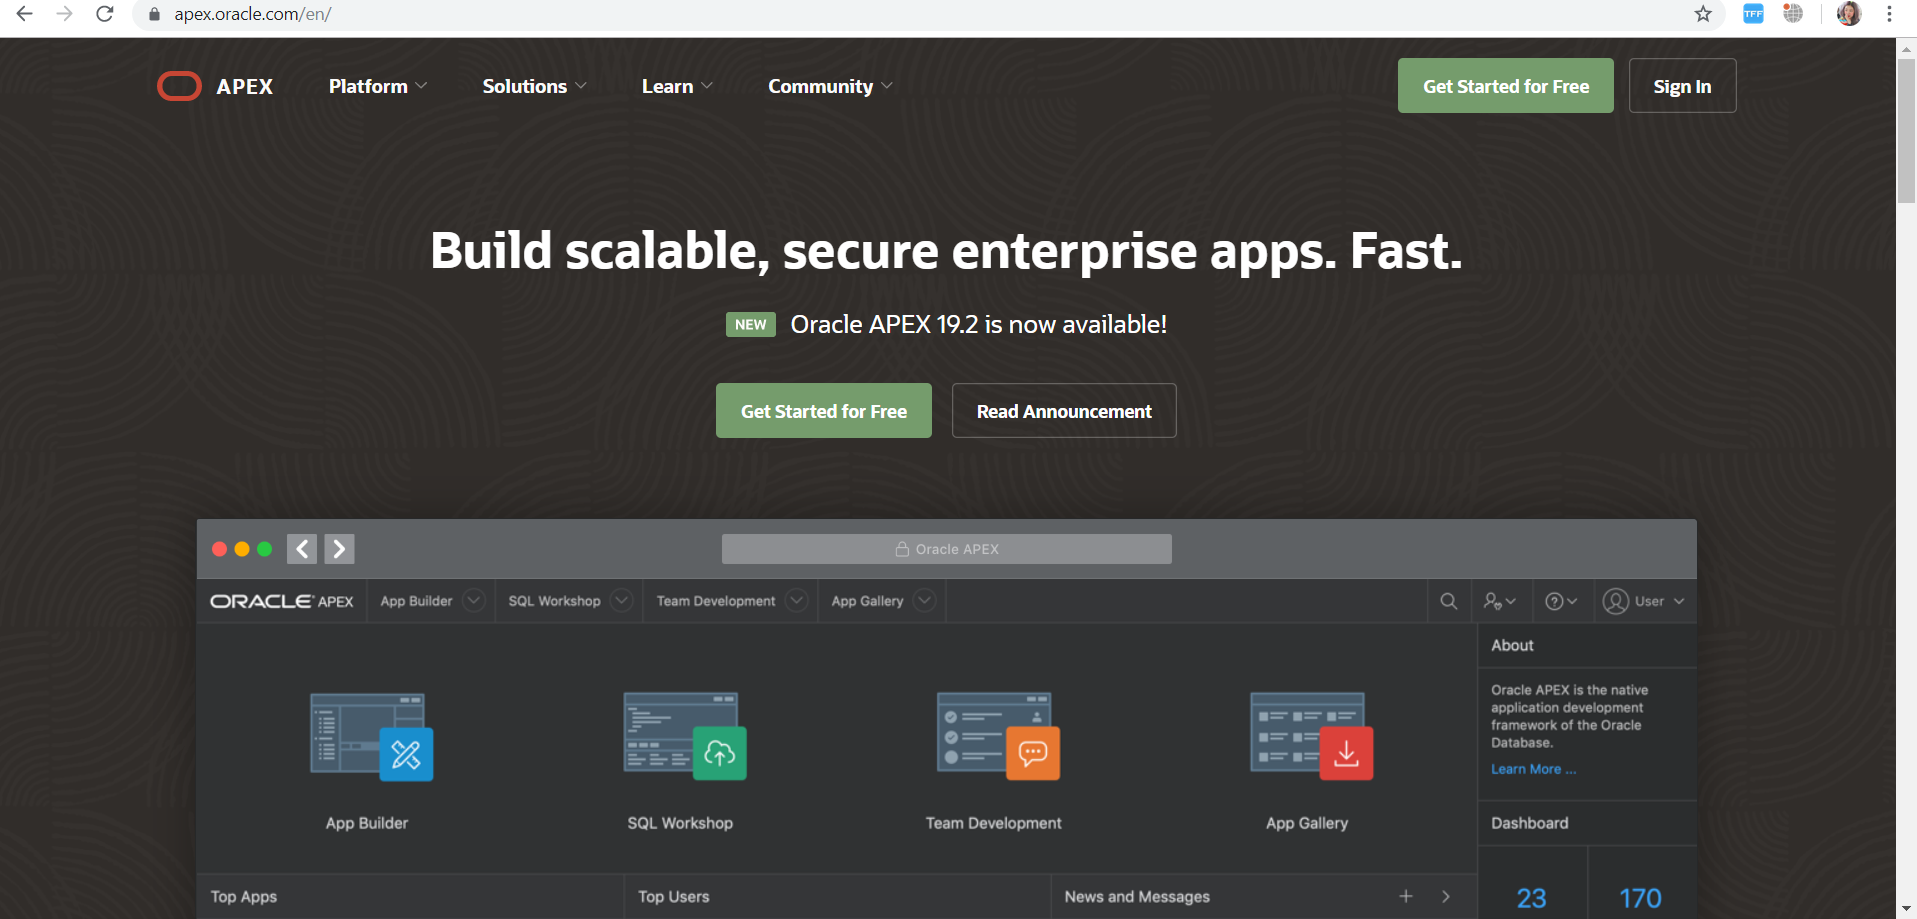
\includegraphics[width=8cm]{GAMBAR/getstarted.PNG}}
        \end{figure}
    \item Berikut adalah tampilan setelah mengklik get started for free, klik request for a workspace dan ikuti langkah selanjutnya dengan mengisi data diri anda.
        \begin{figure}[h]
        \centerline{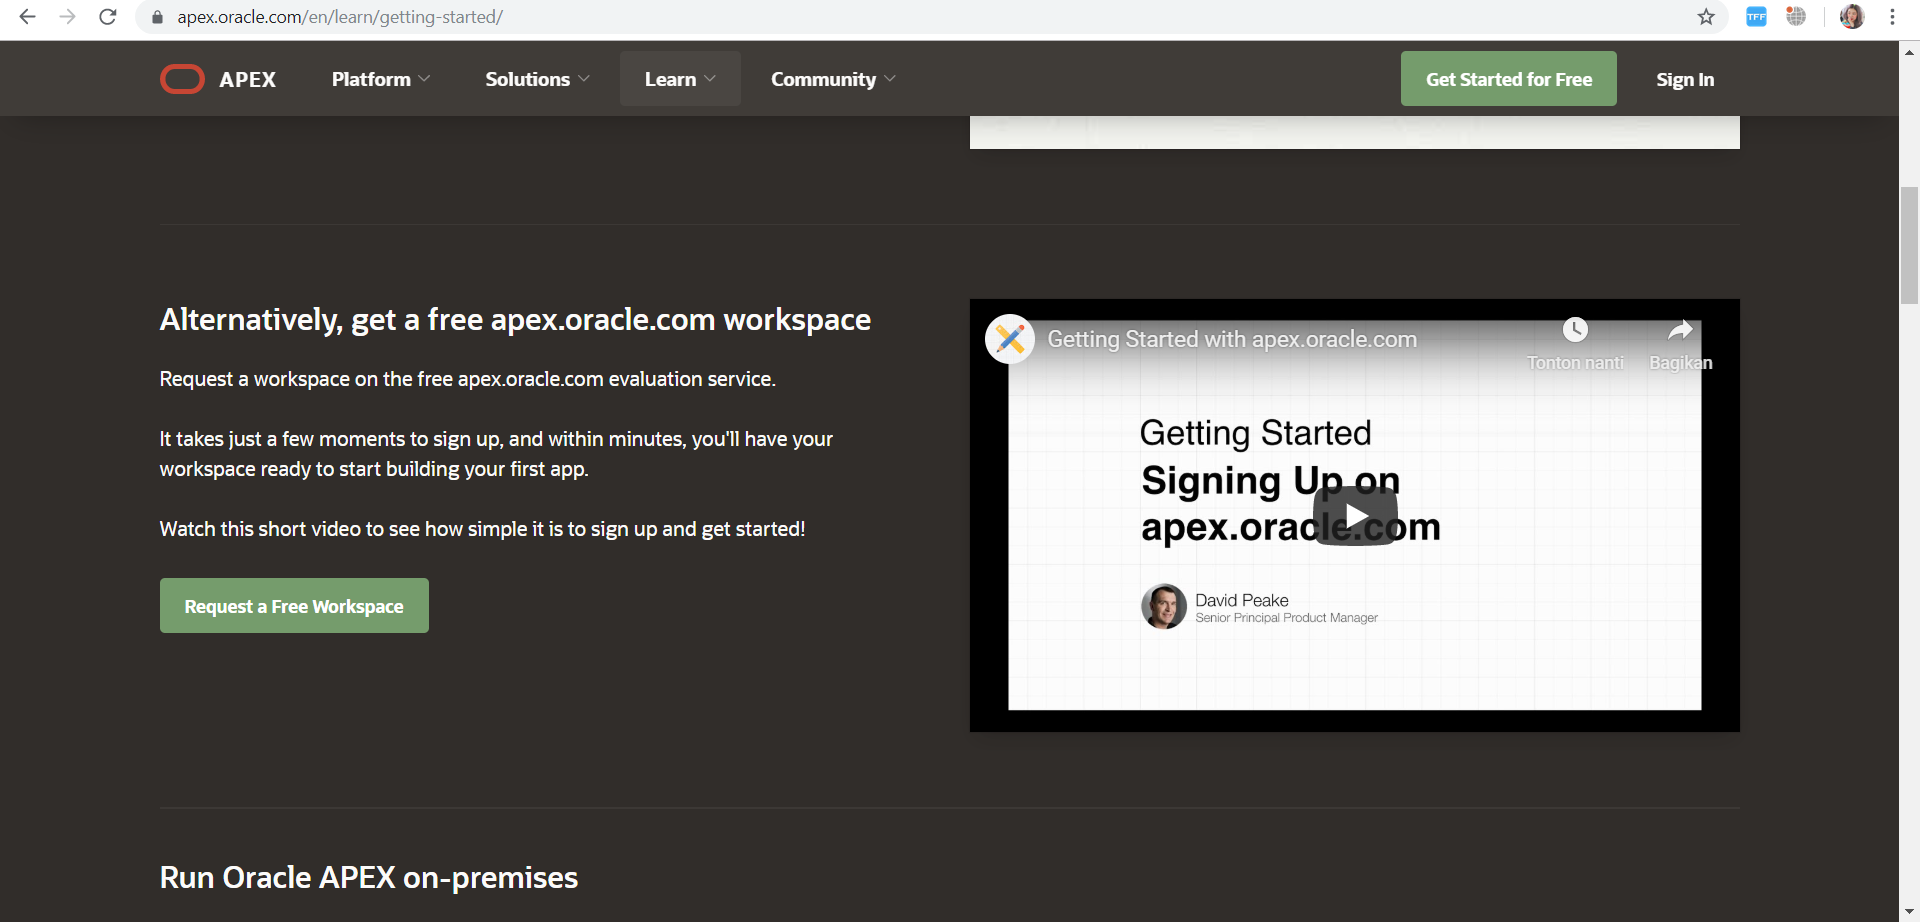
\includegraphics[width=8cm]{GAMBAR/requestws.PNG}}
        \end{figure}
    \item Selanjutnya adalah tampilan untuk Sign In, silahkan isi workspace, username, dan password yang anda miliki.
        \paragraph{}
        \centerline{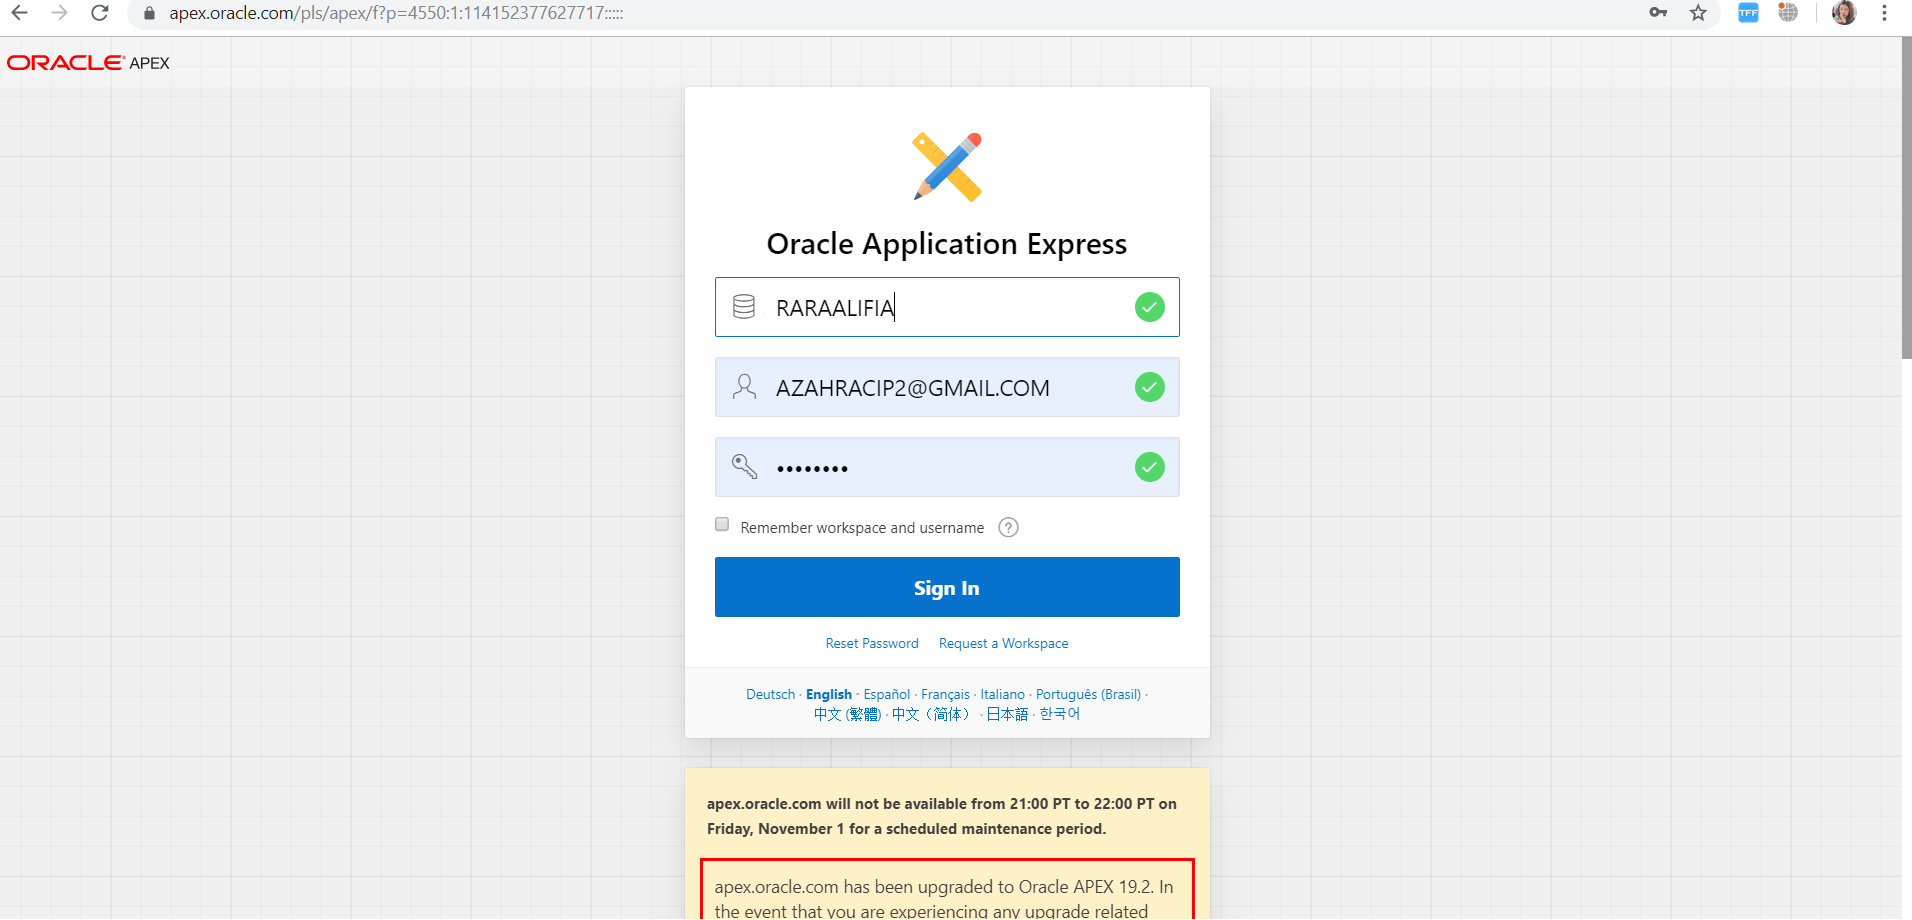
\includegraphics[width=8cm]{GAMBAR/SIGNIN2.PNG}}
    \item Lalu klik app builder
        \paragraph{}
        \centerline{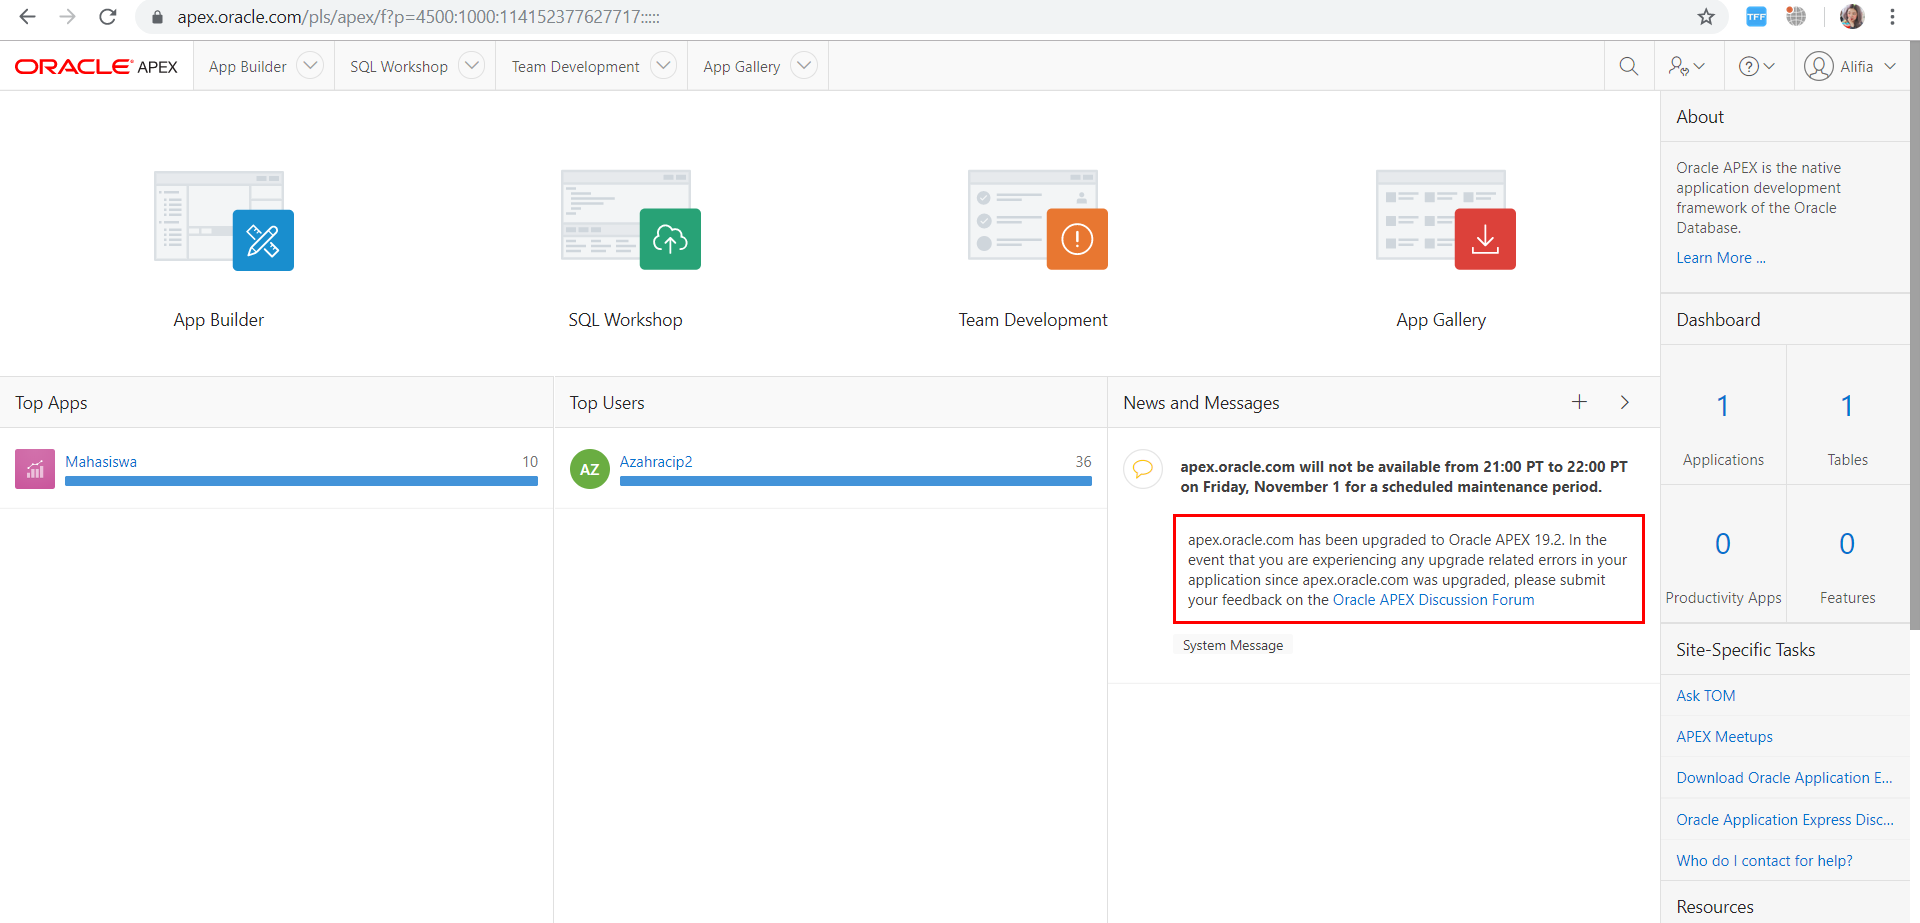
\includegraphics[width=8cm]{GAMBAR/APPBUILDER.PNG}}
    \item Klik create untuk membuat aplikasi
        \begin{figure}[h]
        \centerline{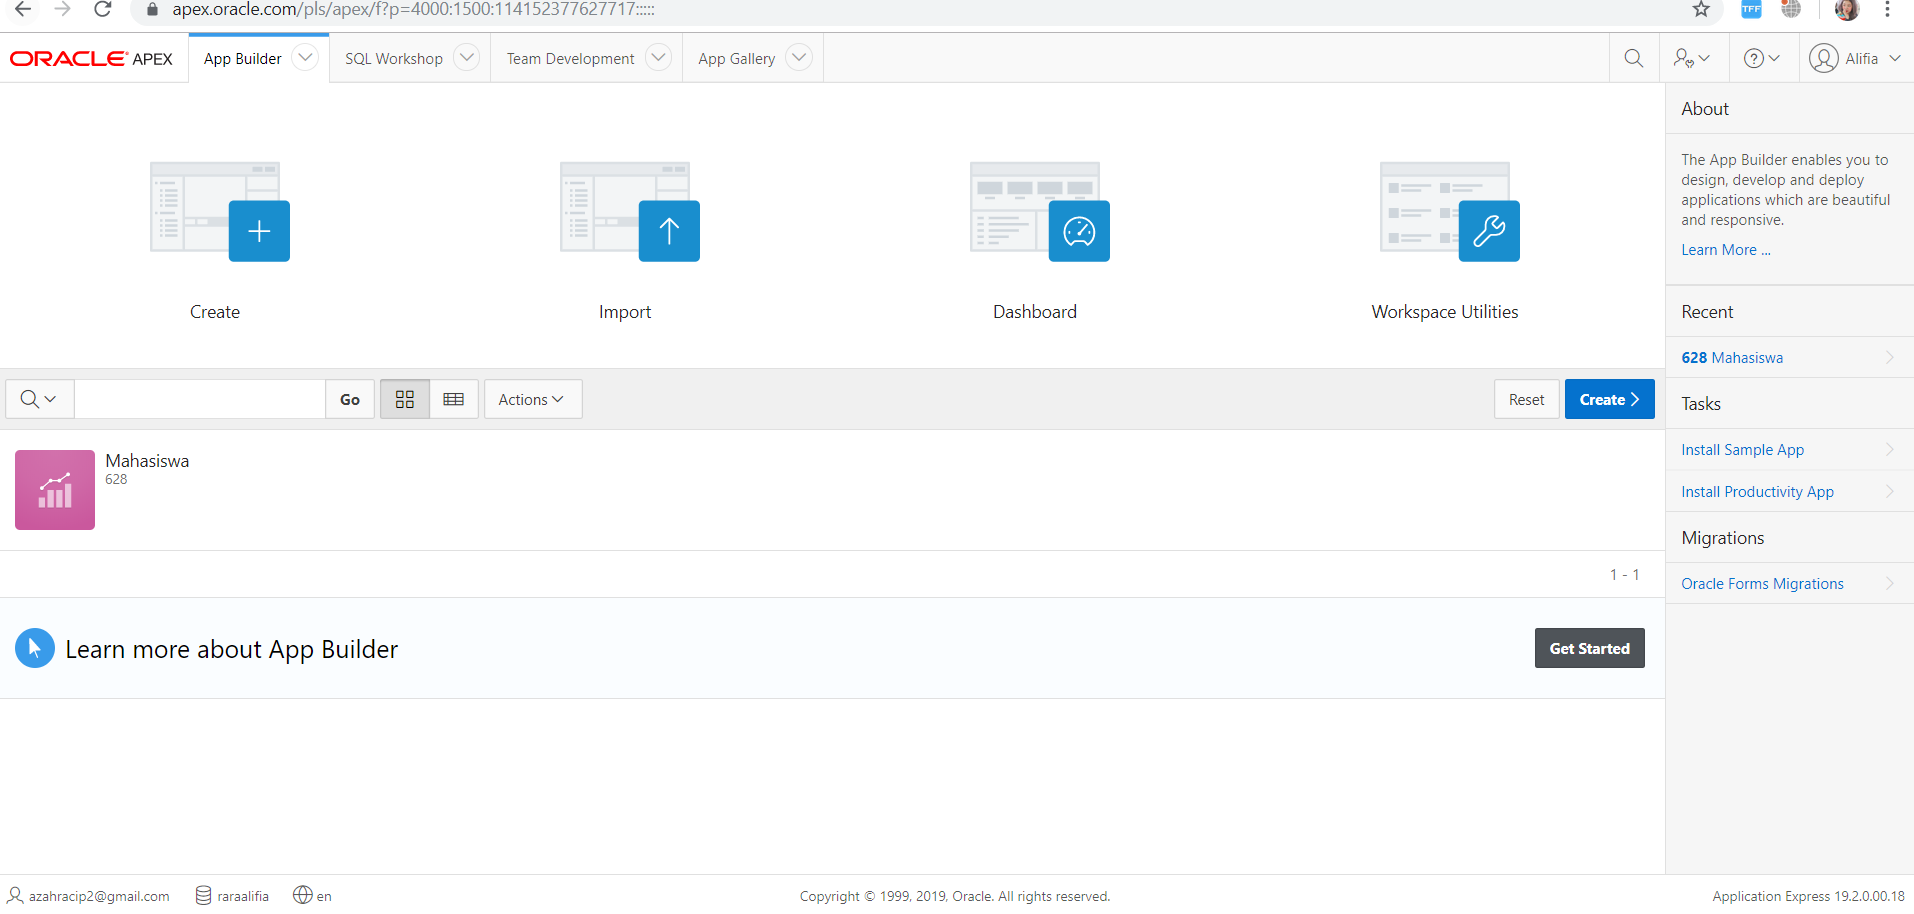
\includegraphics[width=8cm]{GAMBAR/CREATE.PNG}}
        \end{figure}
    \item Pilih opsi from a file lalu upload file yang akan anda masukkan dalam aplikasi anda, pastikan ekstensinya \textit{csv.}
        \begin{figure}[h]
        \centerline{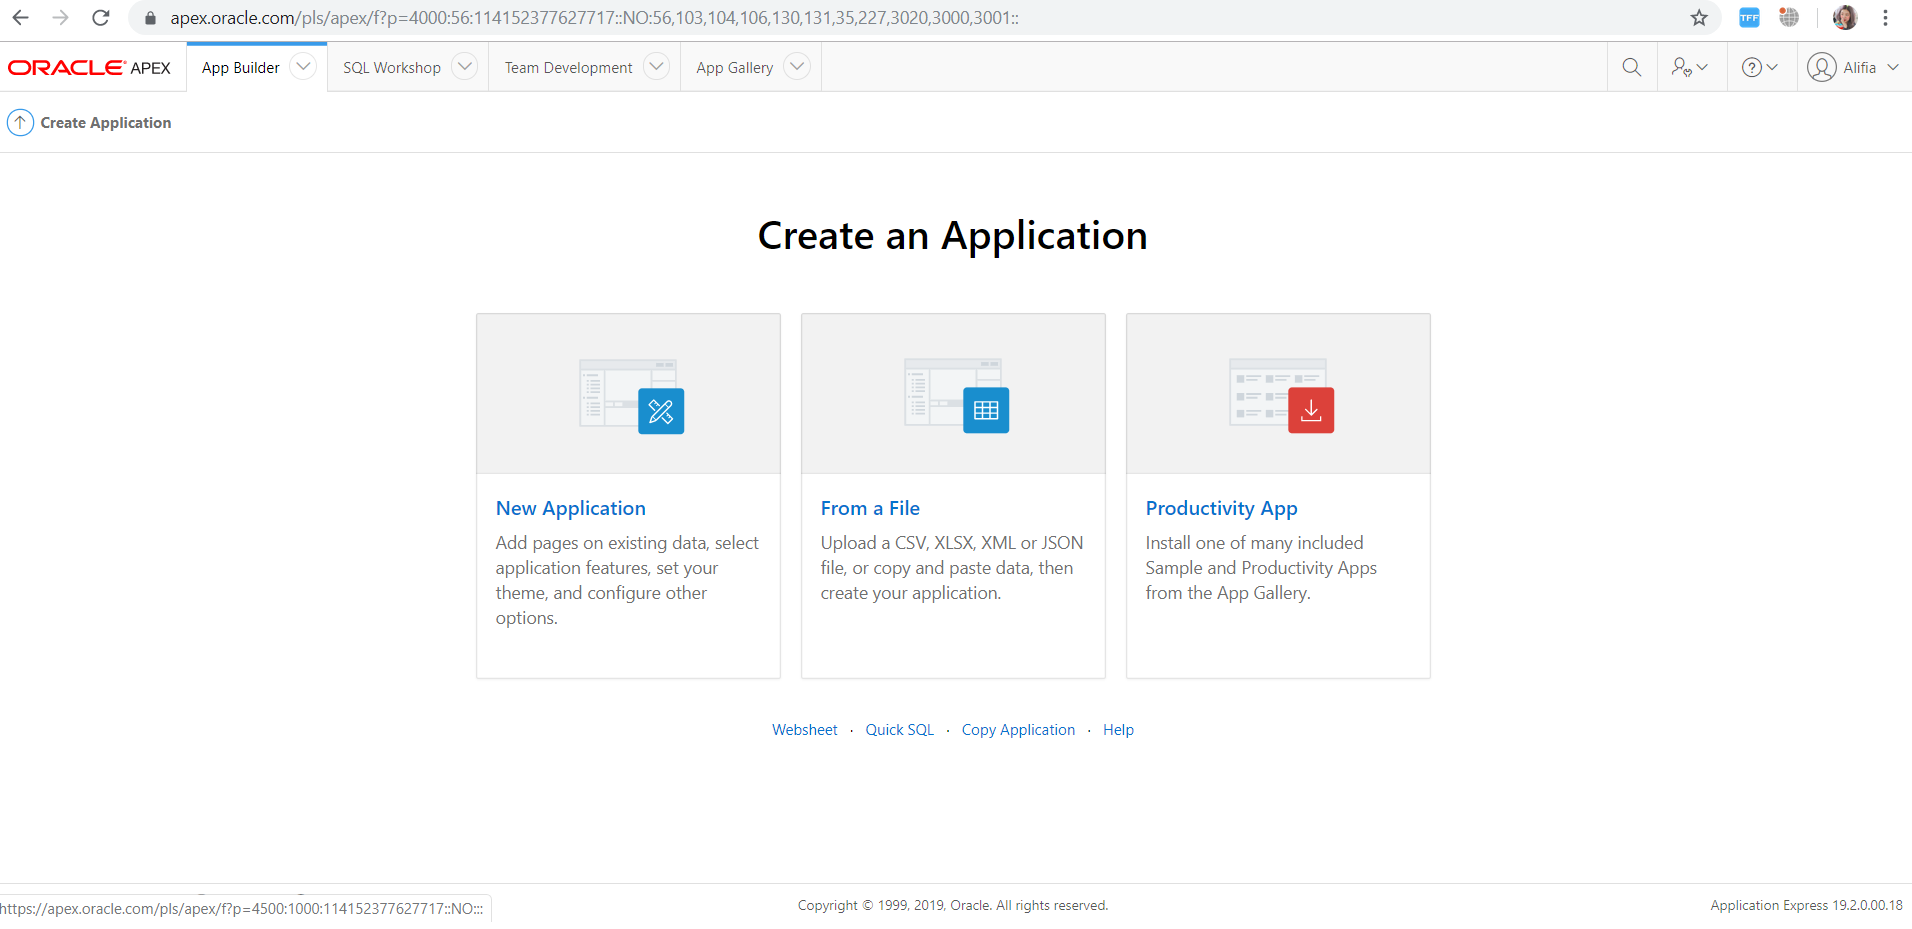
\includegraphics[width=8cm]{GAMBAR/FROMAFILE.PNG}}
        \end{figure}
        \paragraph{}
        \centerline{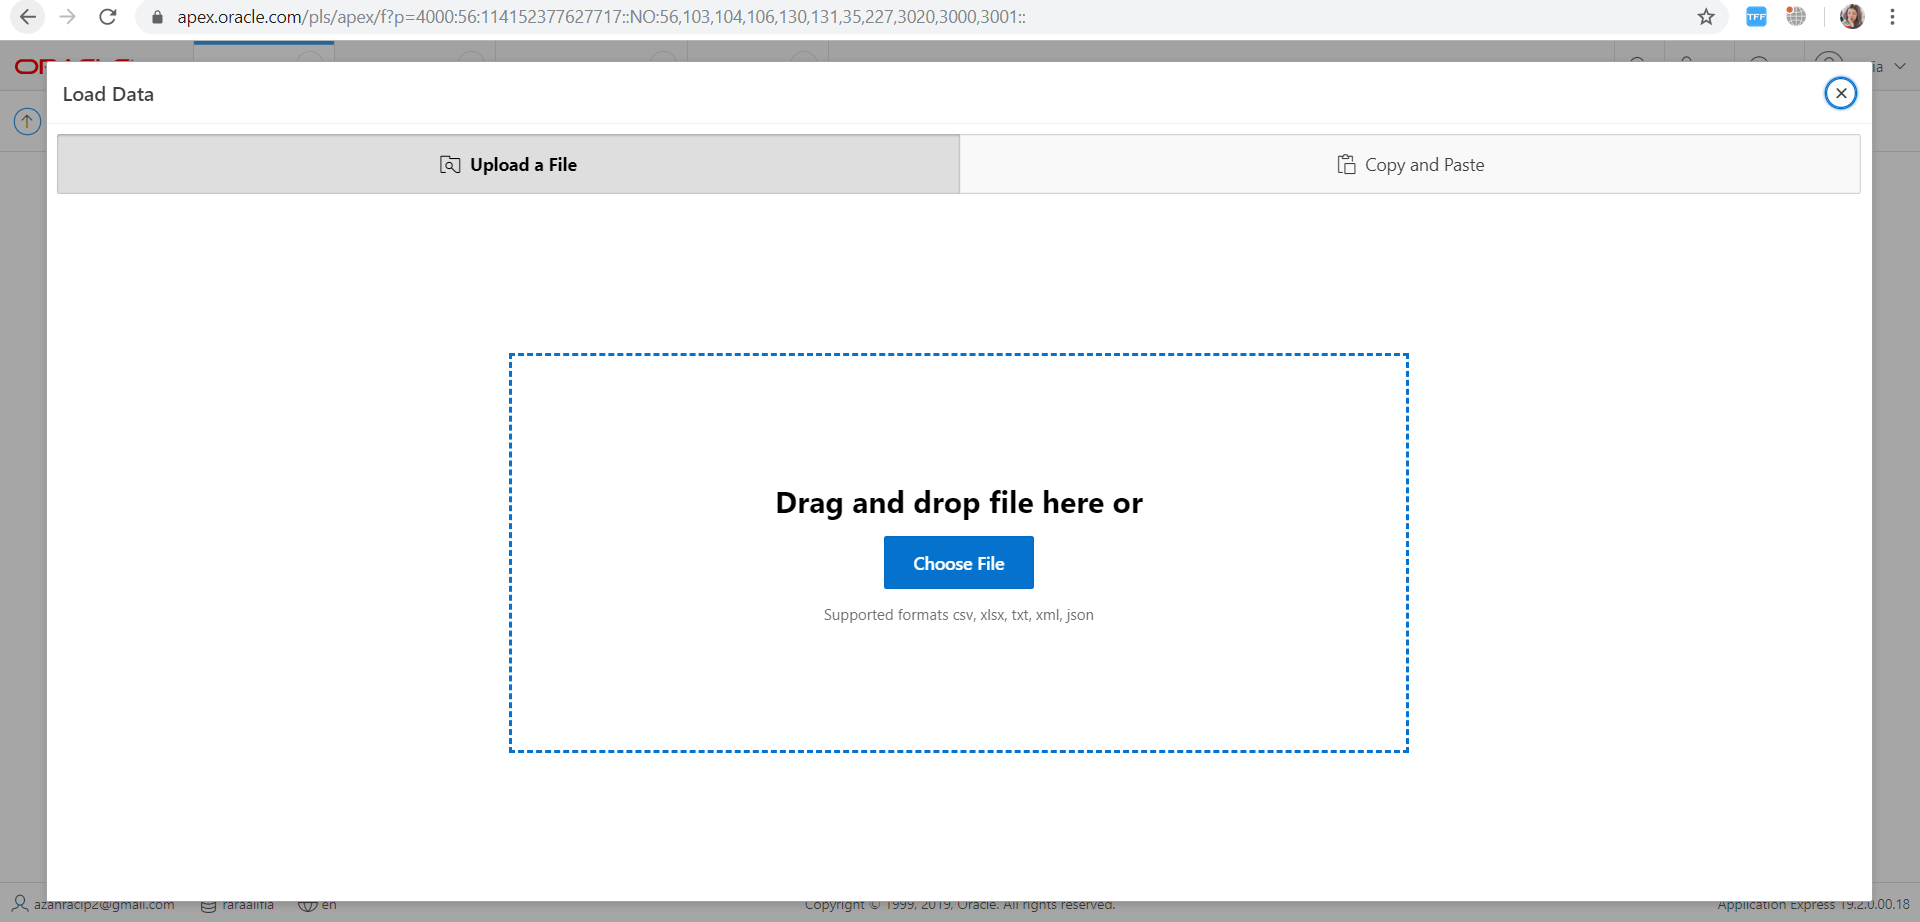
\includegraphics[width=8cm]{GAMBAR/CHOOSEFILE.PNG}}
    \item Disini saya akan mengupload File Data.
        \paragraph{}
        \centerline{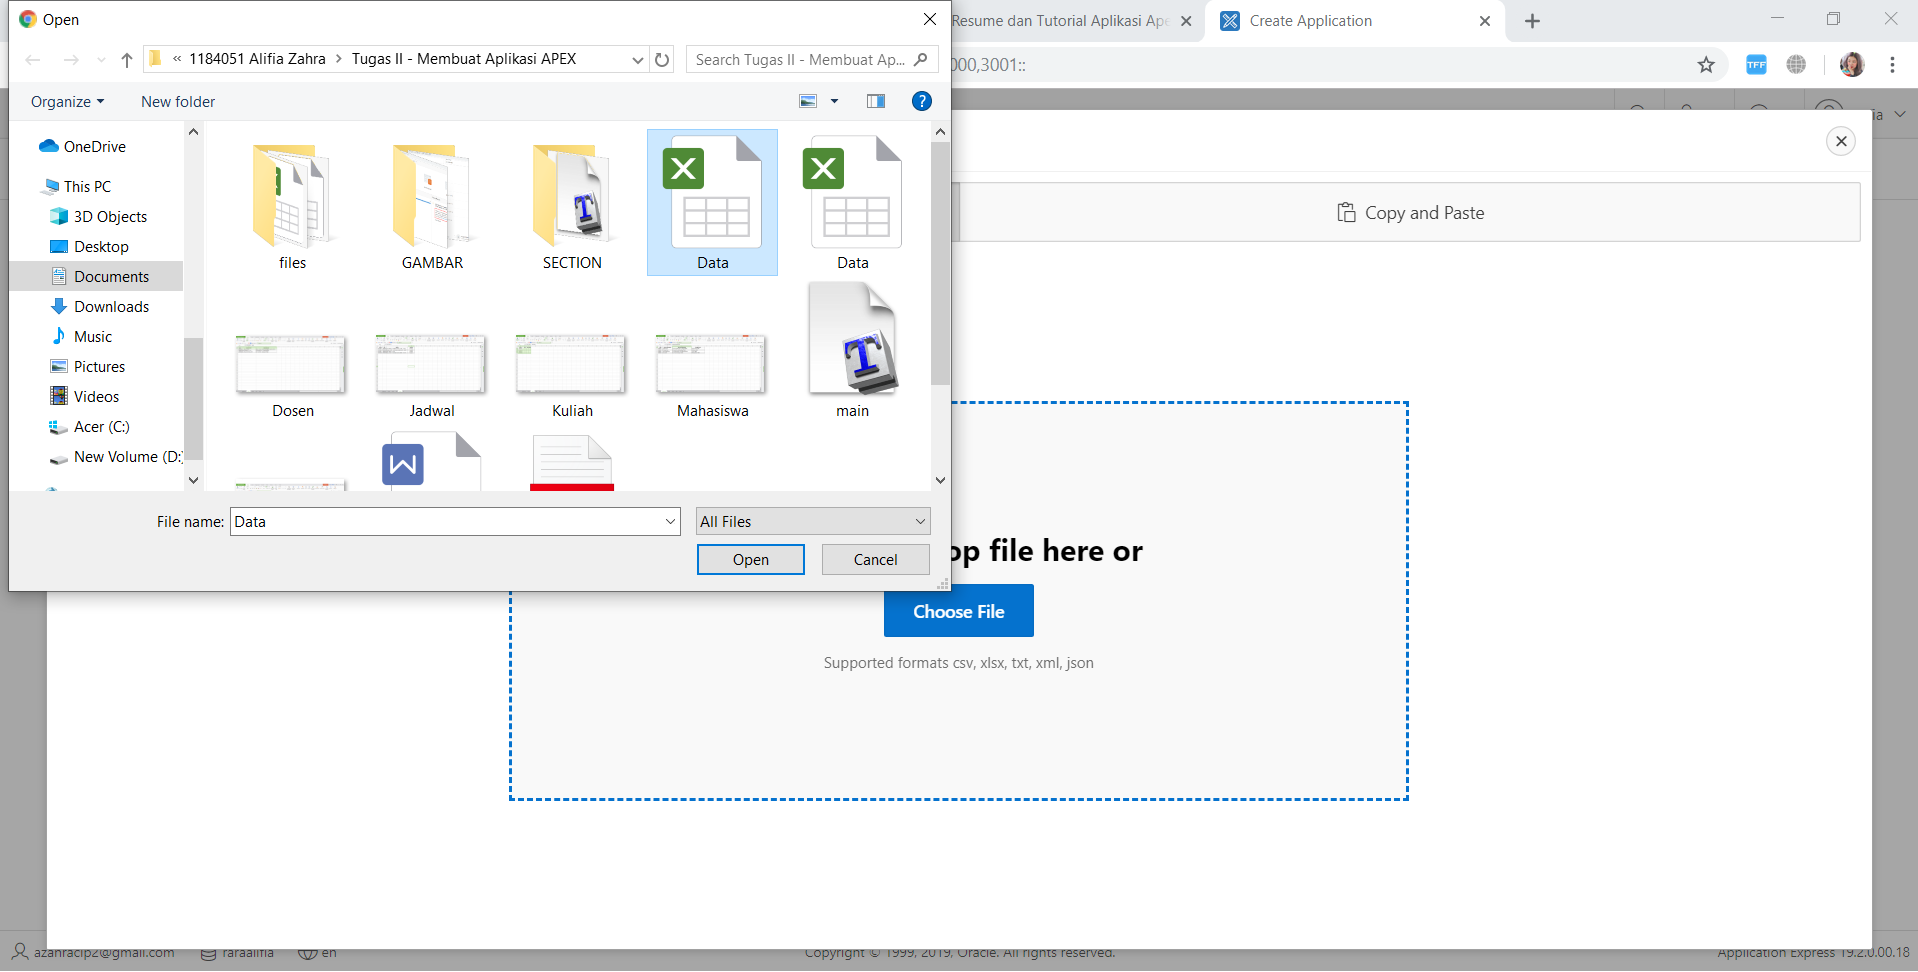
\includegraphics[width=8cm]{Figures/Data.PNG}}
    \item Setelah itu isi tabel sesuai dengan urutan tabel yang berada di dalam file yaitu dimulai dari table Mahasiswa. Lalu klik configure dan save changes.
        \begin{figure}[h]
        \centerline{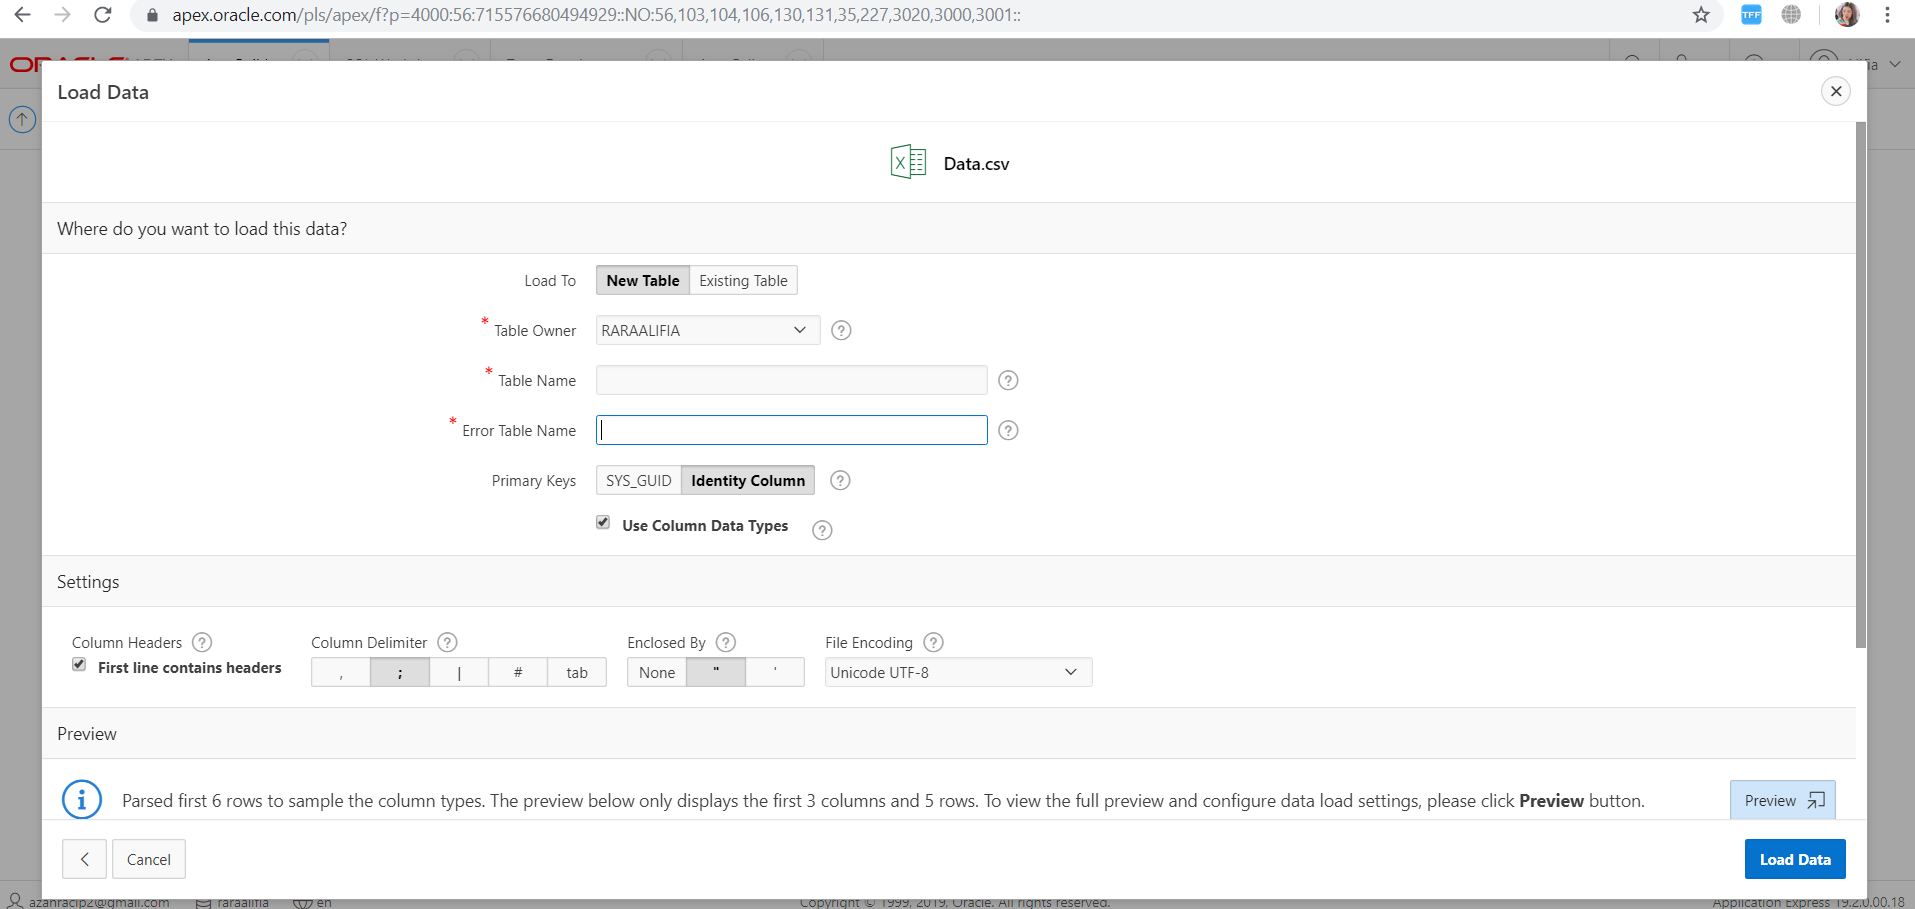
\includegraphics[width=8cm]{Figures/table_name.PNG}}
        \end{figure}
        \begin{figure}[h]
        \centerline{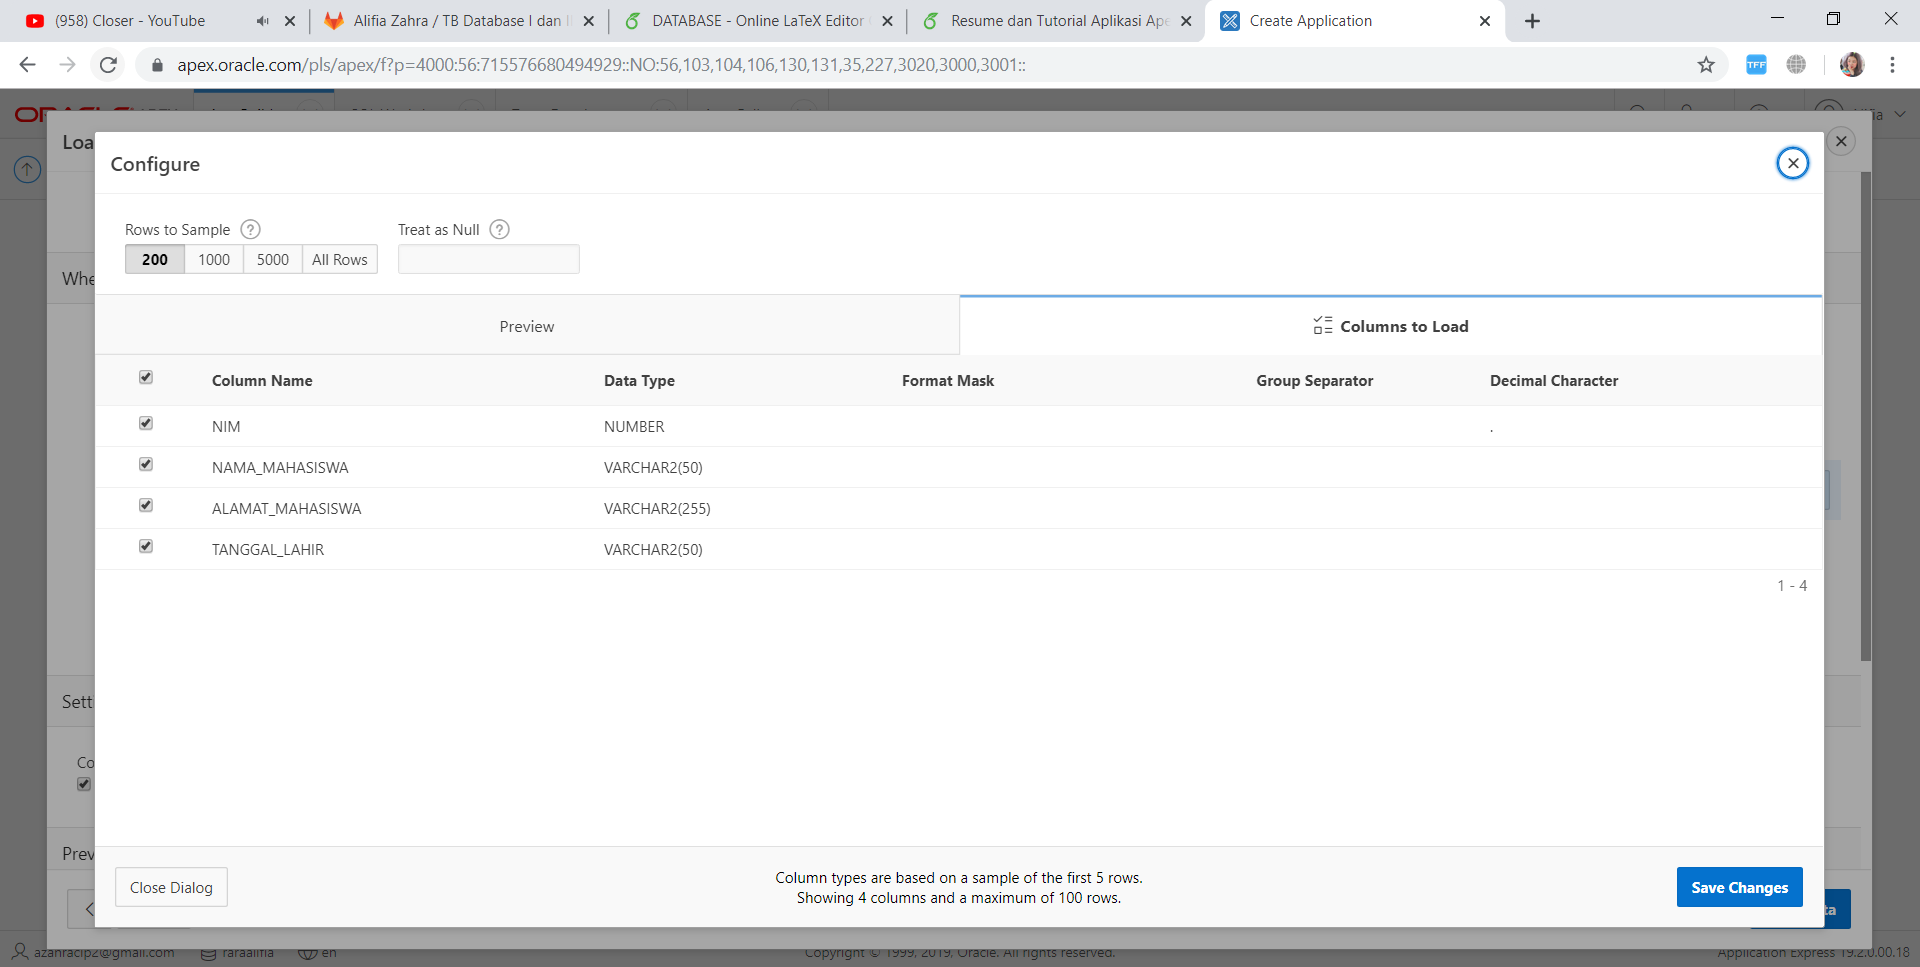
\includegraphics[width=8cm]{Figures/table_mahasiswa.PNG}}
        \end{figure}
    \item Lalu Klik Load Data dan ulangi langkah sebelumnya untuk memasukkan tabel selanjutnya yaitu tabel dosen. Lalu klik configure dan save changes.
        \begin{figure}[h]
        \centerline{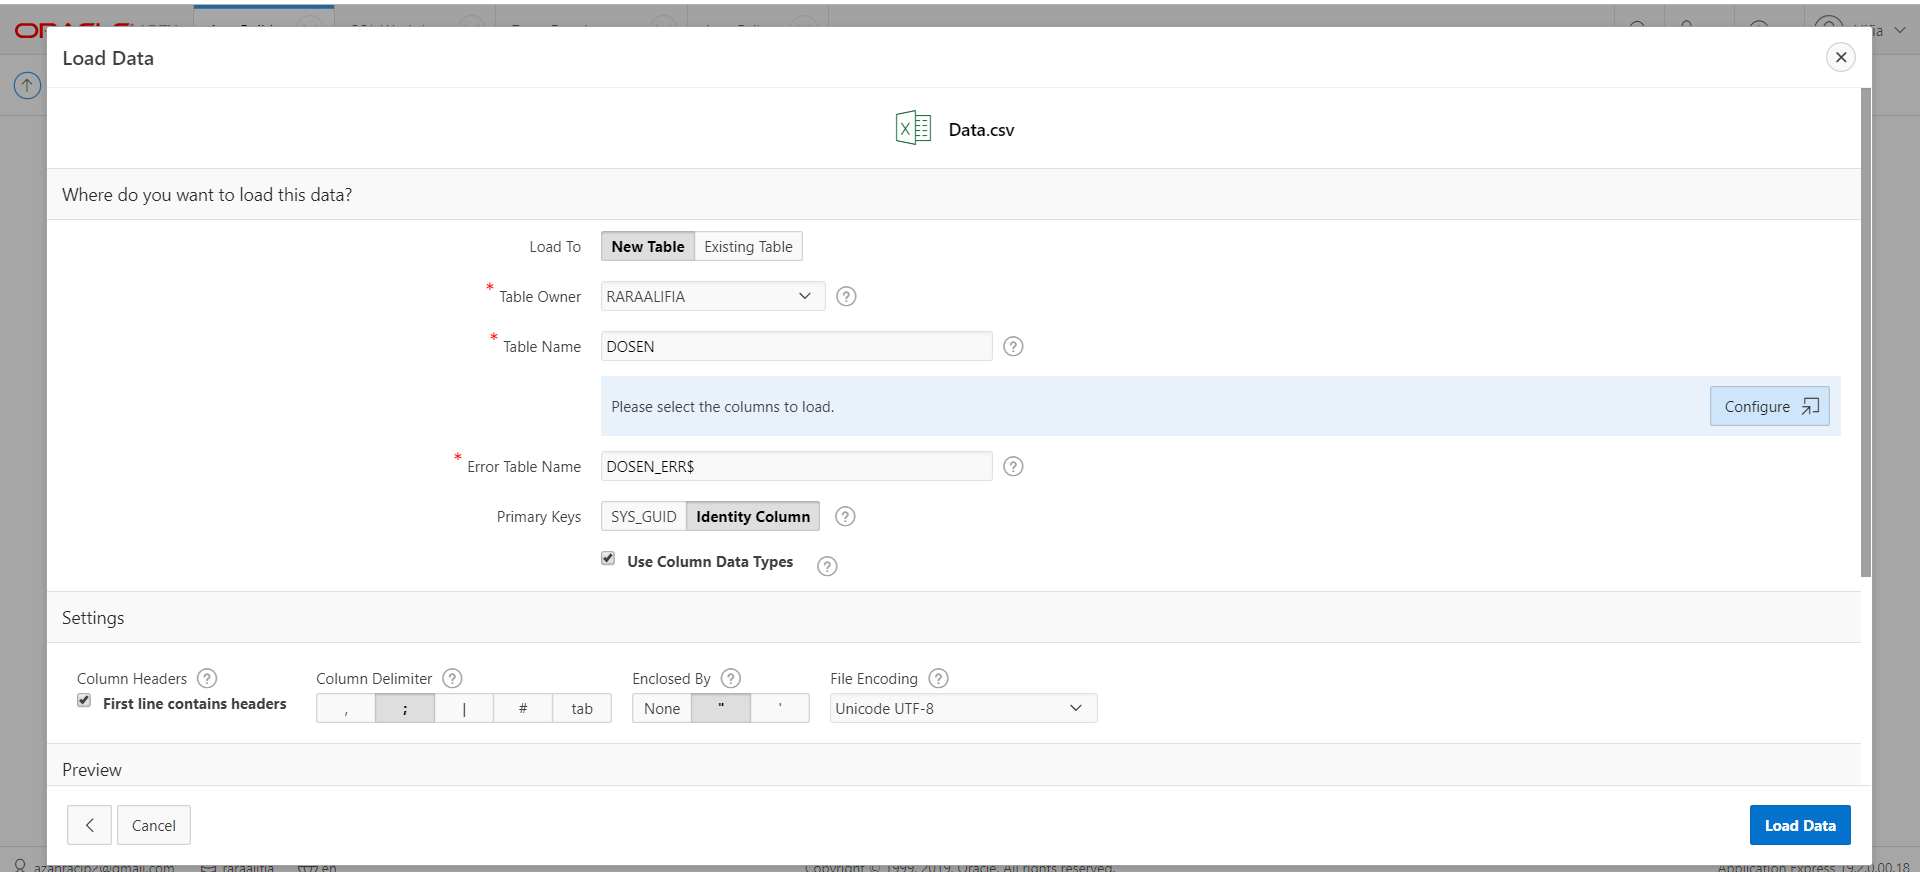
\includegraphics[width=8cm]{Figures/tabel_dosen.PNG}}
        \end{figure}
        \begin{figure}[h]
        \centerline{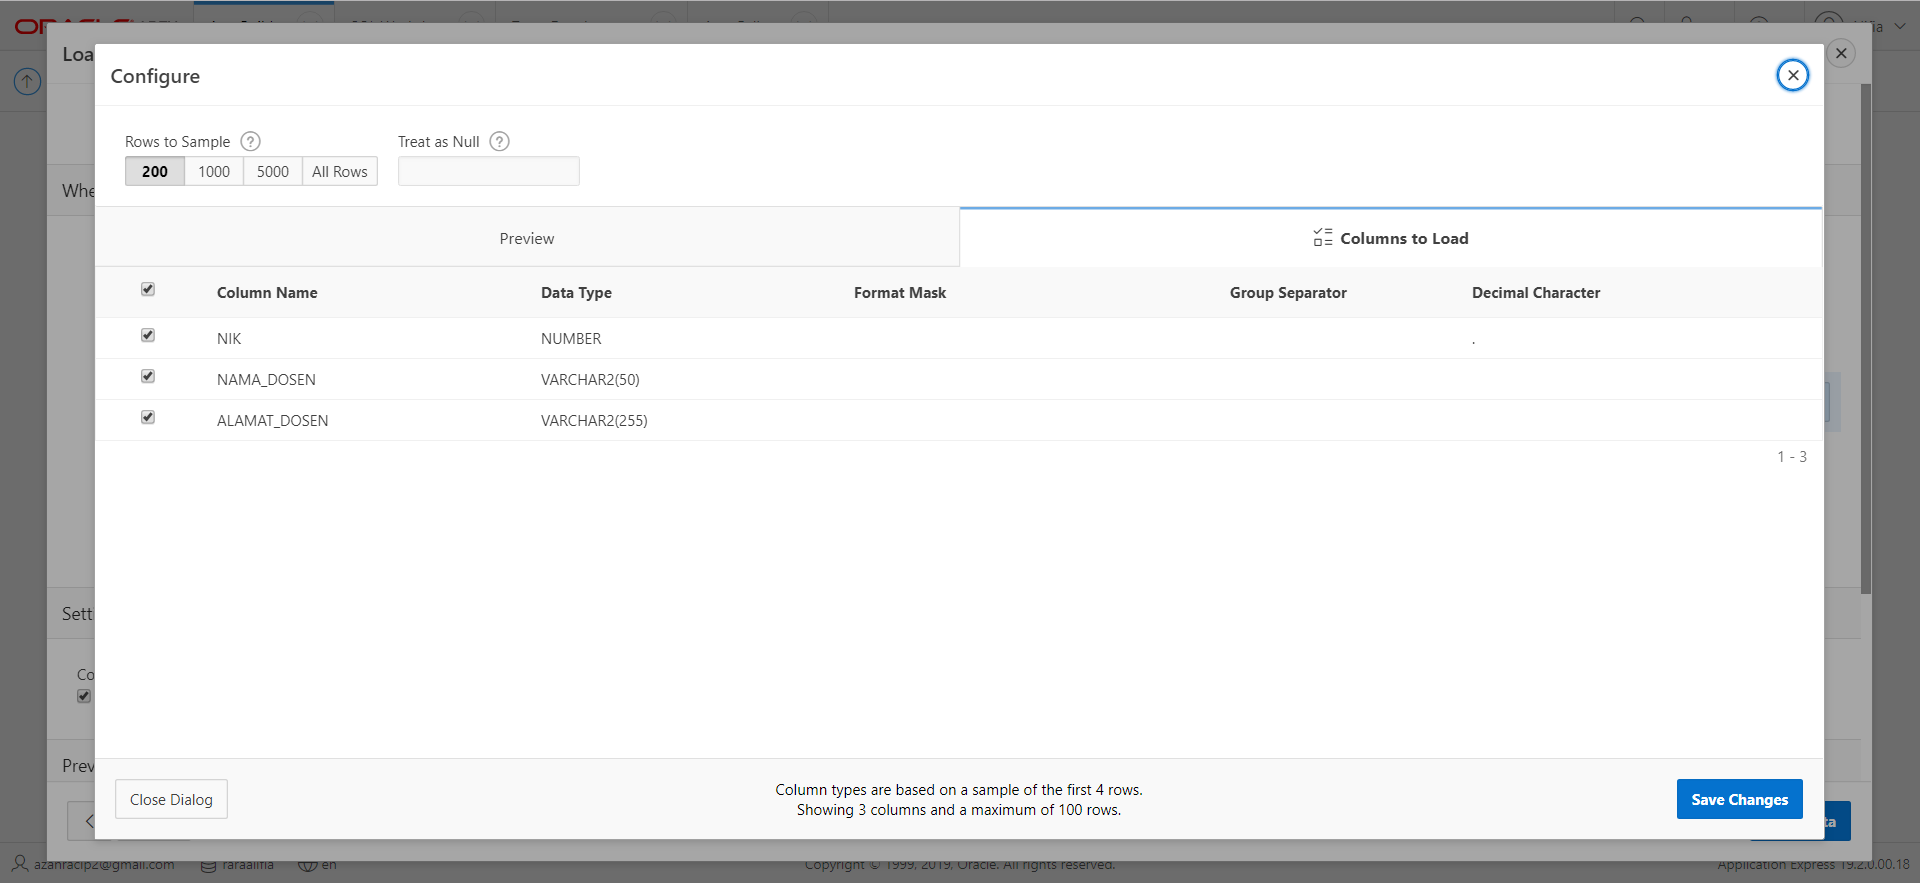
\includegraphics[width=8cm]{Figures/configdosen.PNG}}
        \end{figure}
    \item Lalu Klik Load Data dan ulangi langkah sebelumnya untuk memasukkan tabel selanjutnya yaitu tabel nilai. Lalu klik configure dan save changes.
        \begin{figure}[h]
        \centerline{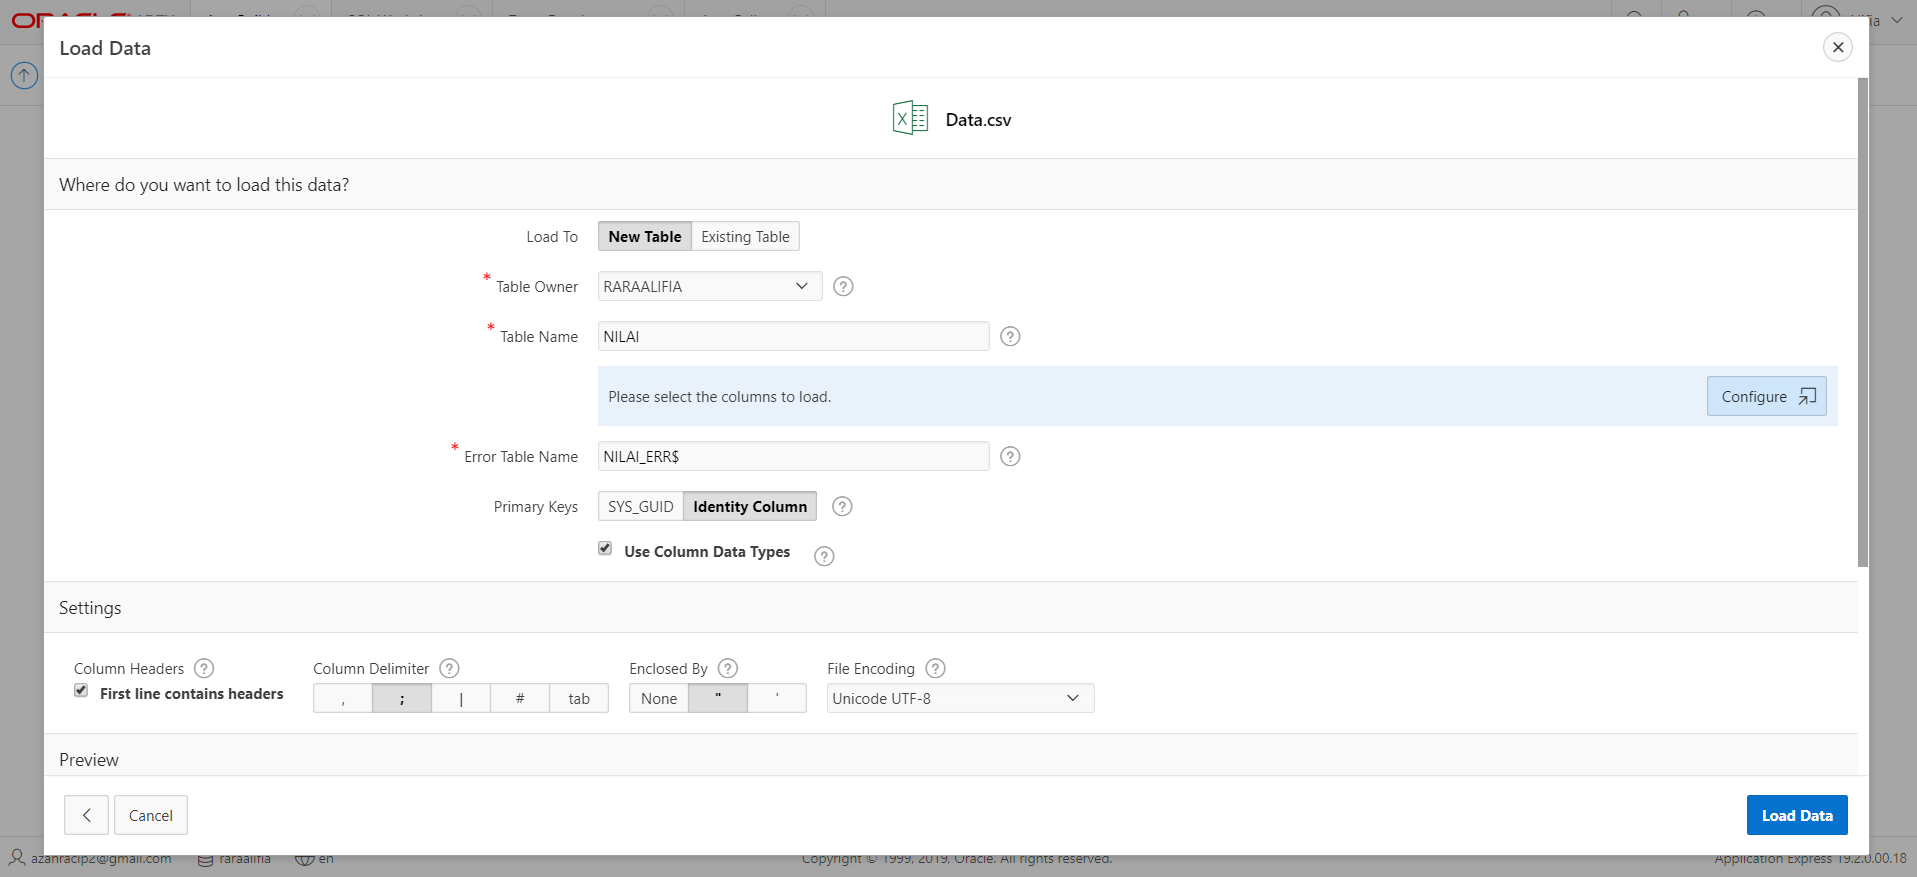
\includegraphics[width=8cm]{Figures/tabel_nilai.PNG}}
        \end{figure}
        \paragraph{}
        \centerline{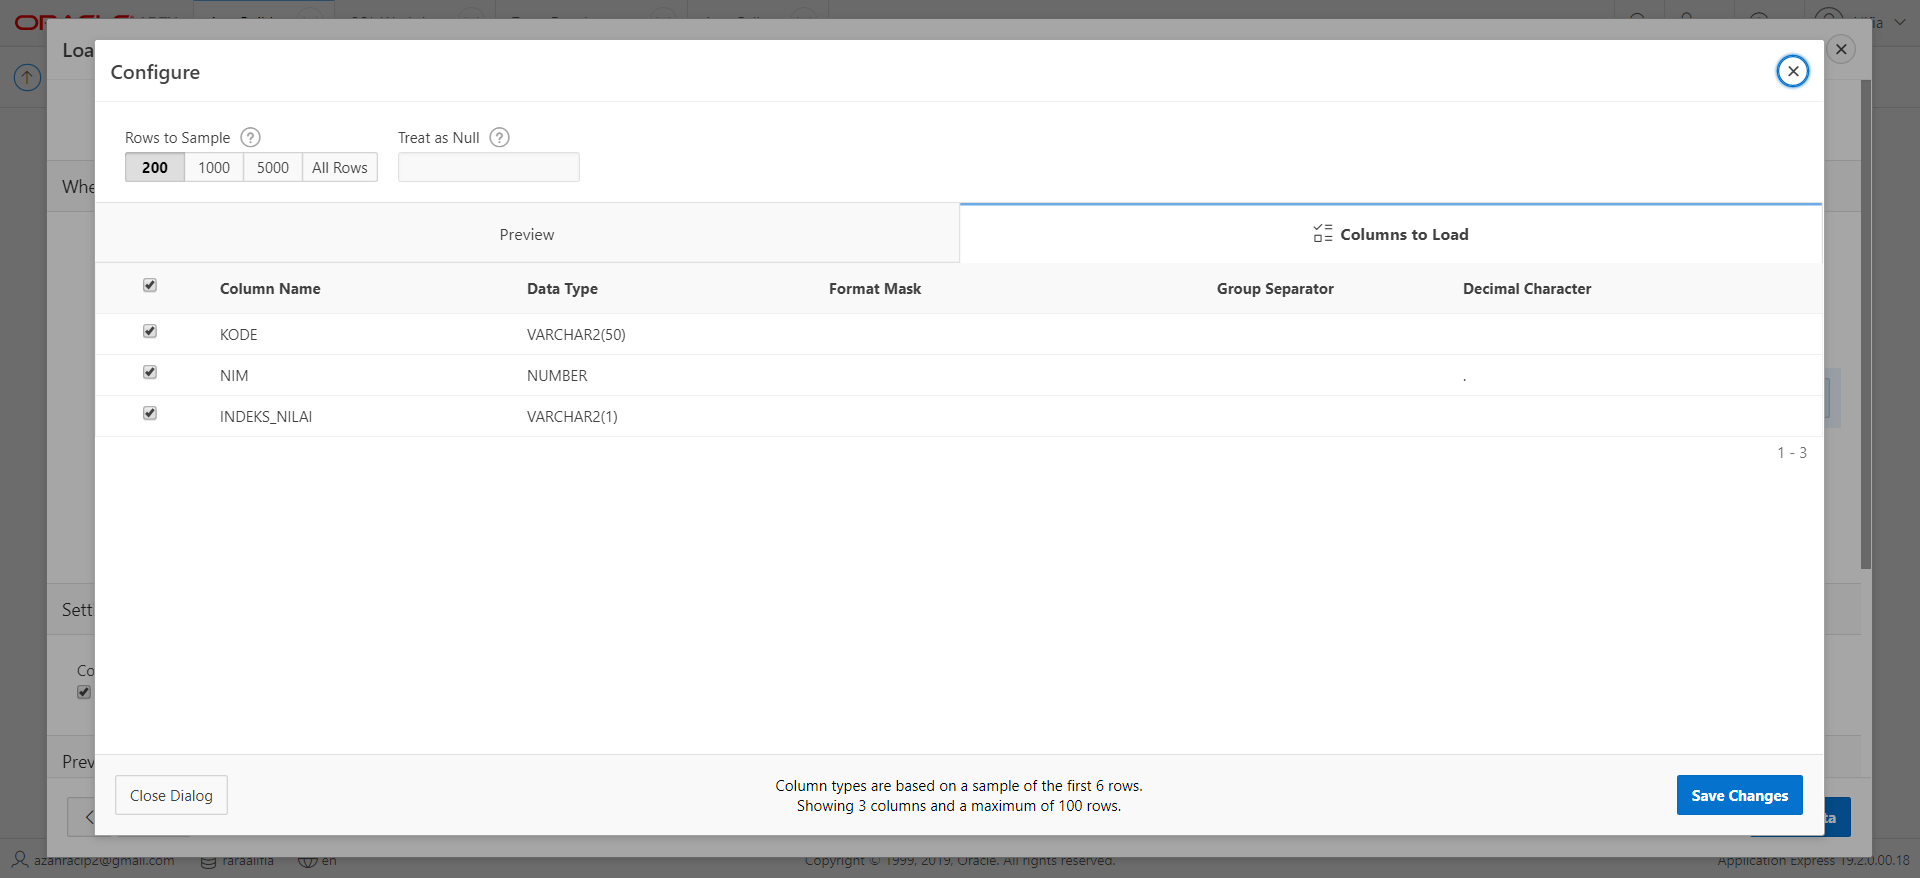
\includegraphics[width=8cm]{Figures/confignilai.PNG}}
    \item Lalu Klik Load Data dan ulangi langkah sebelumnya untuk memasukkan tabel selanjutnya yaitu tabel kuliah. Lalu klik configure dan save changes.
        \begin{figure}[h]
        \centerline{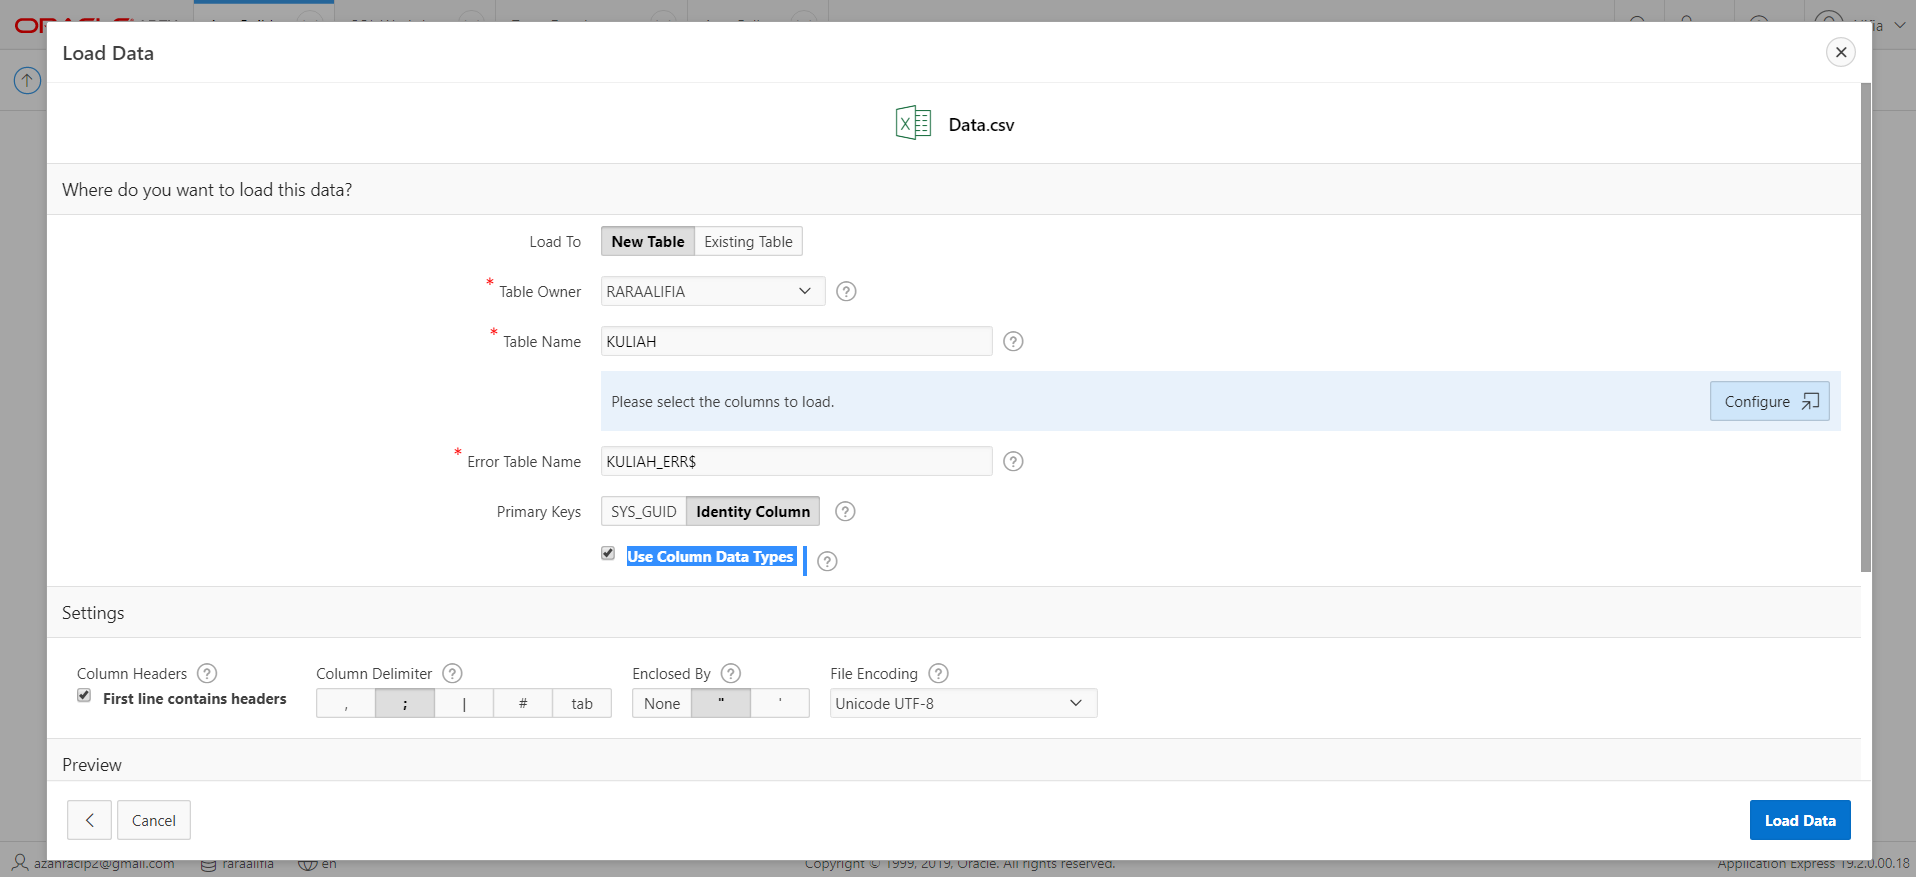
\includegraphics[width=8cm]{Figures/tabel_kuliah.PNG}}
        \end{figure}
        \begin{figure}[h]
        \centerline{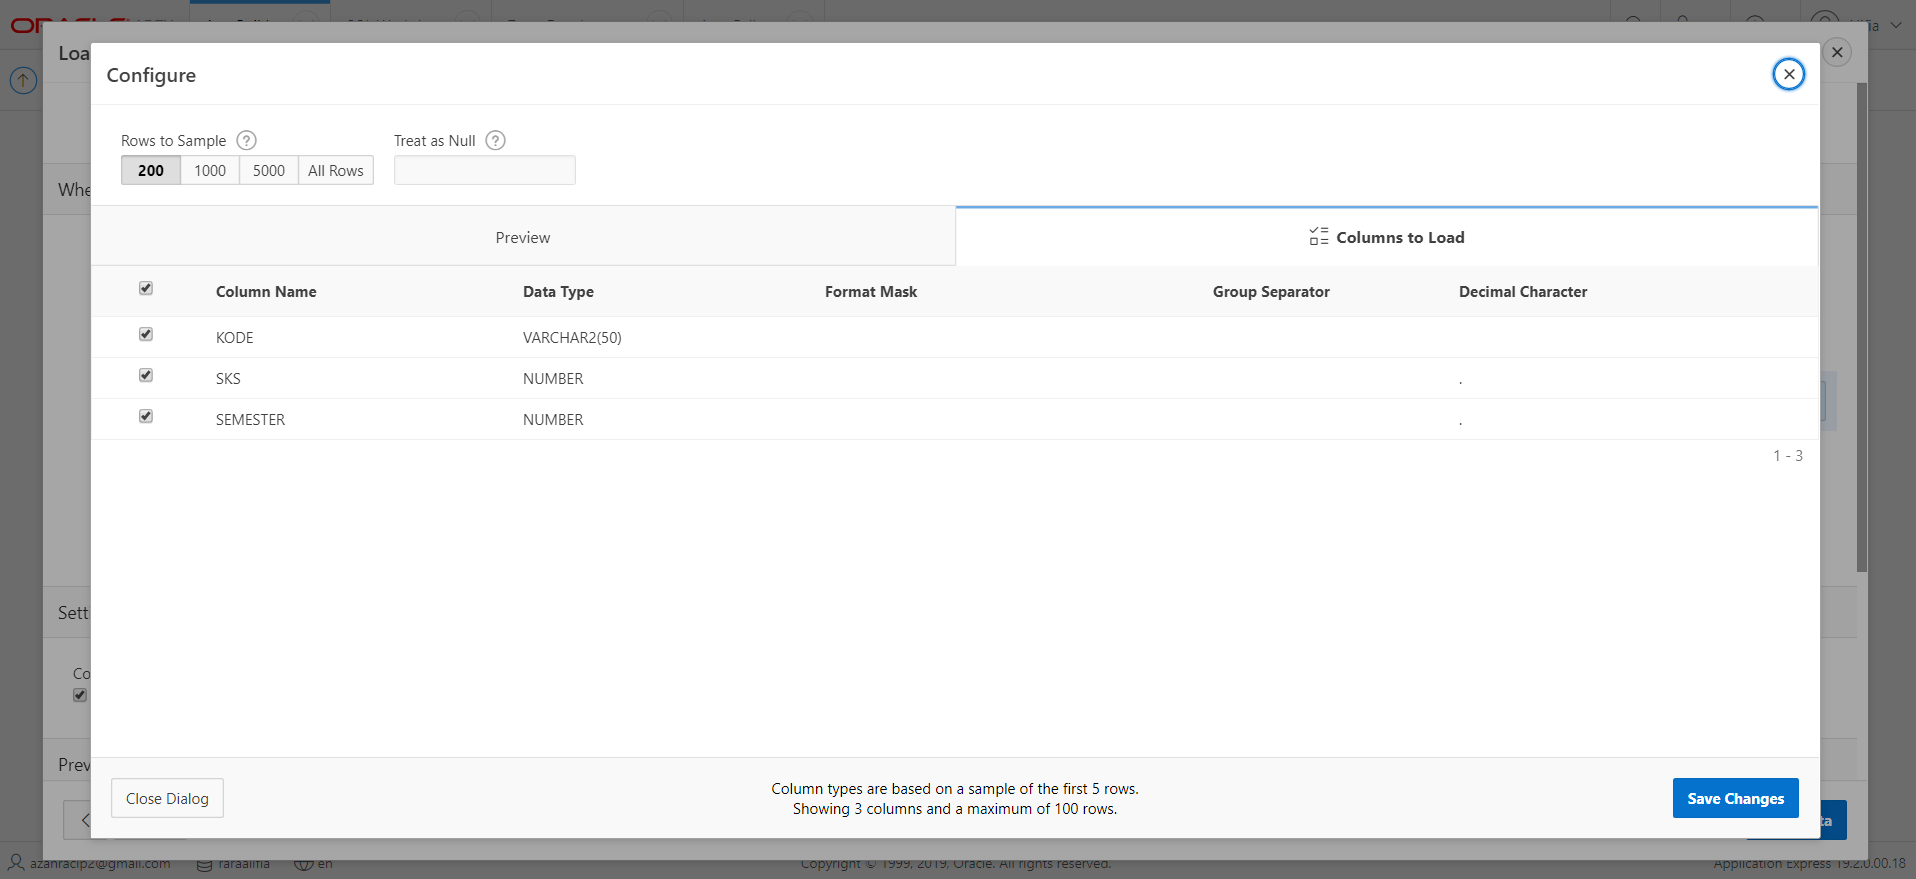
\includegraphics[width=8cm]{Figures/configkuliah.PNG}}
        \end{figure}
    \item Lalu Klik Load Data dan ulangi langkah sebelumnya untuk memasukkan tabel selanjutnya yaitu tabel jadwal. Lalu klik configure dan save changes.
        \begin{figure}[h]
        \centerline{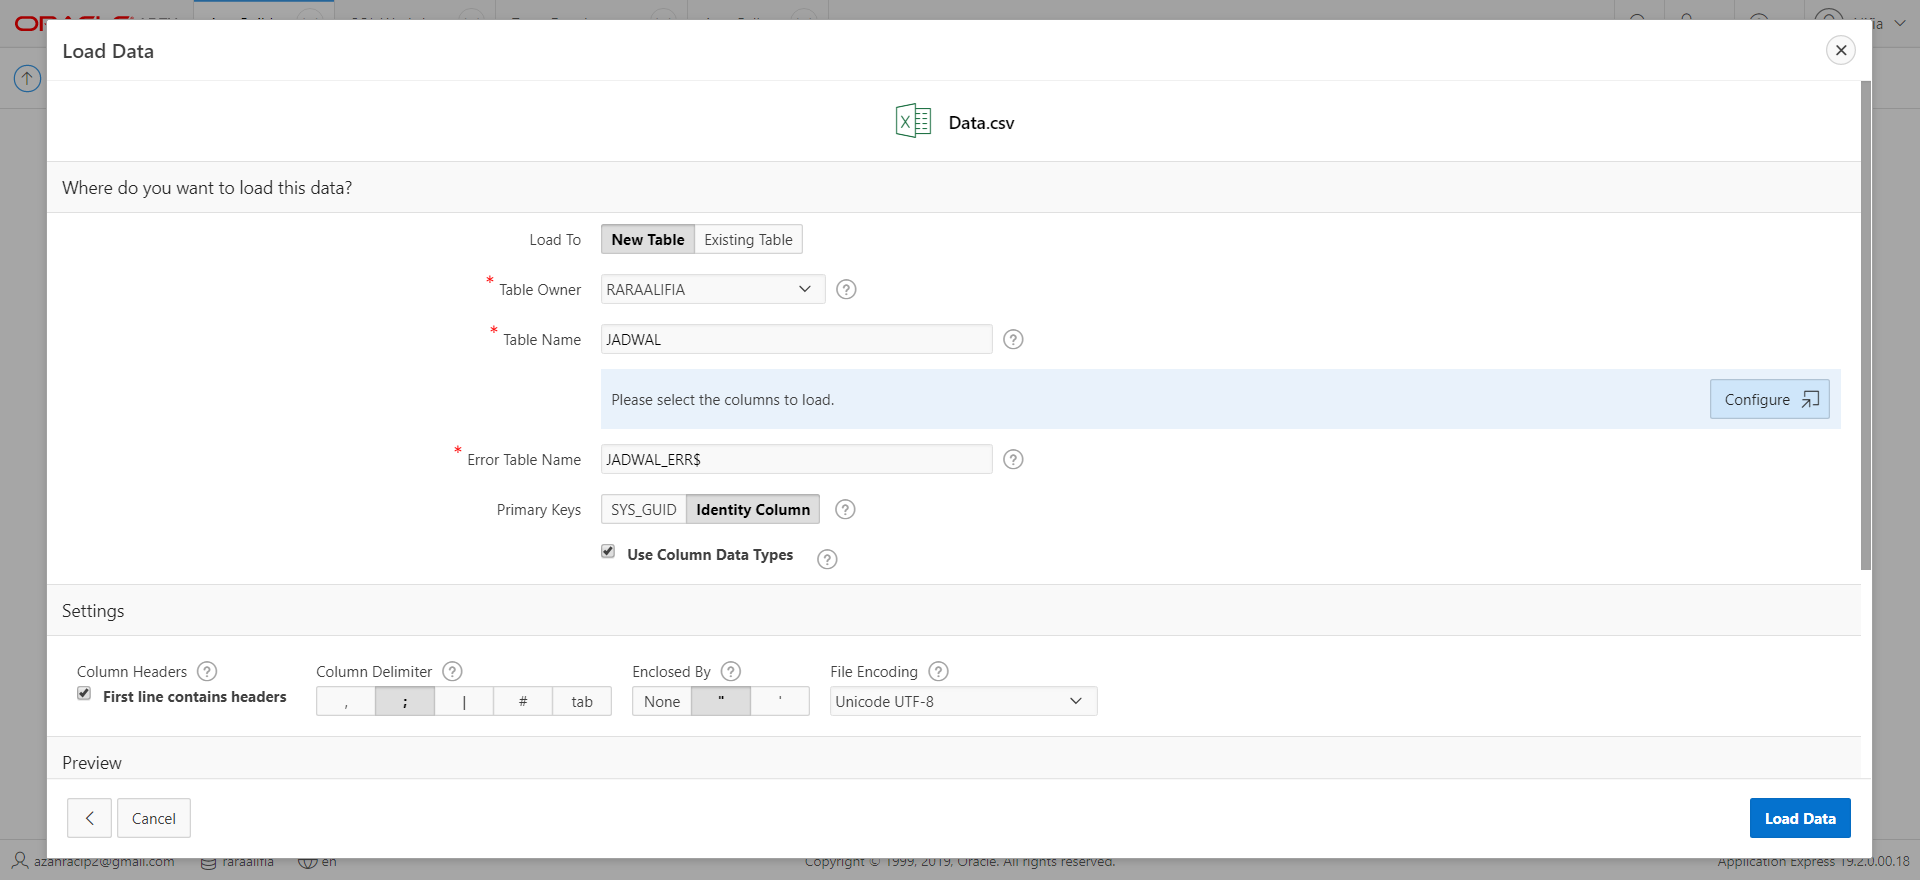
\includegraphics[width=8cm]{Figures/tabel_jadwal.PNG}}
        \end{figure}
        \paragraph{}
        \centerline{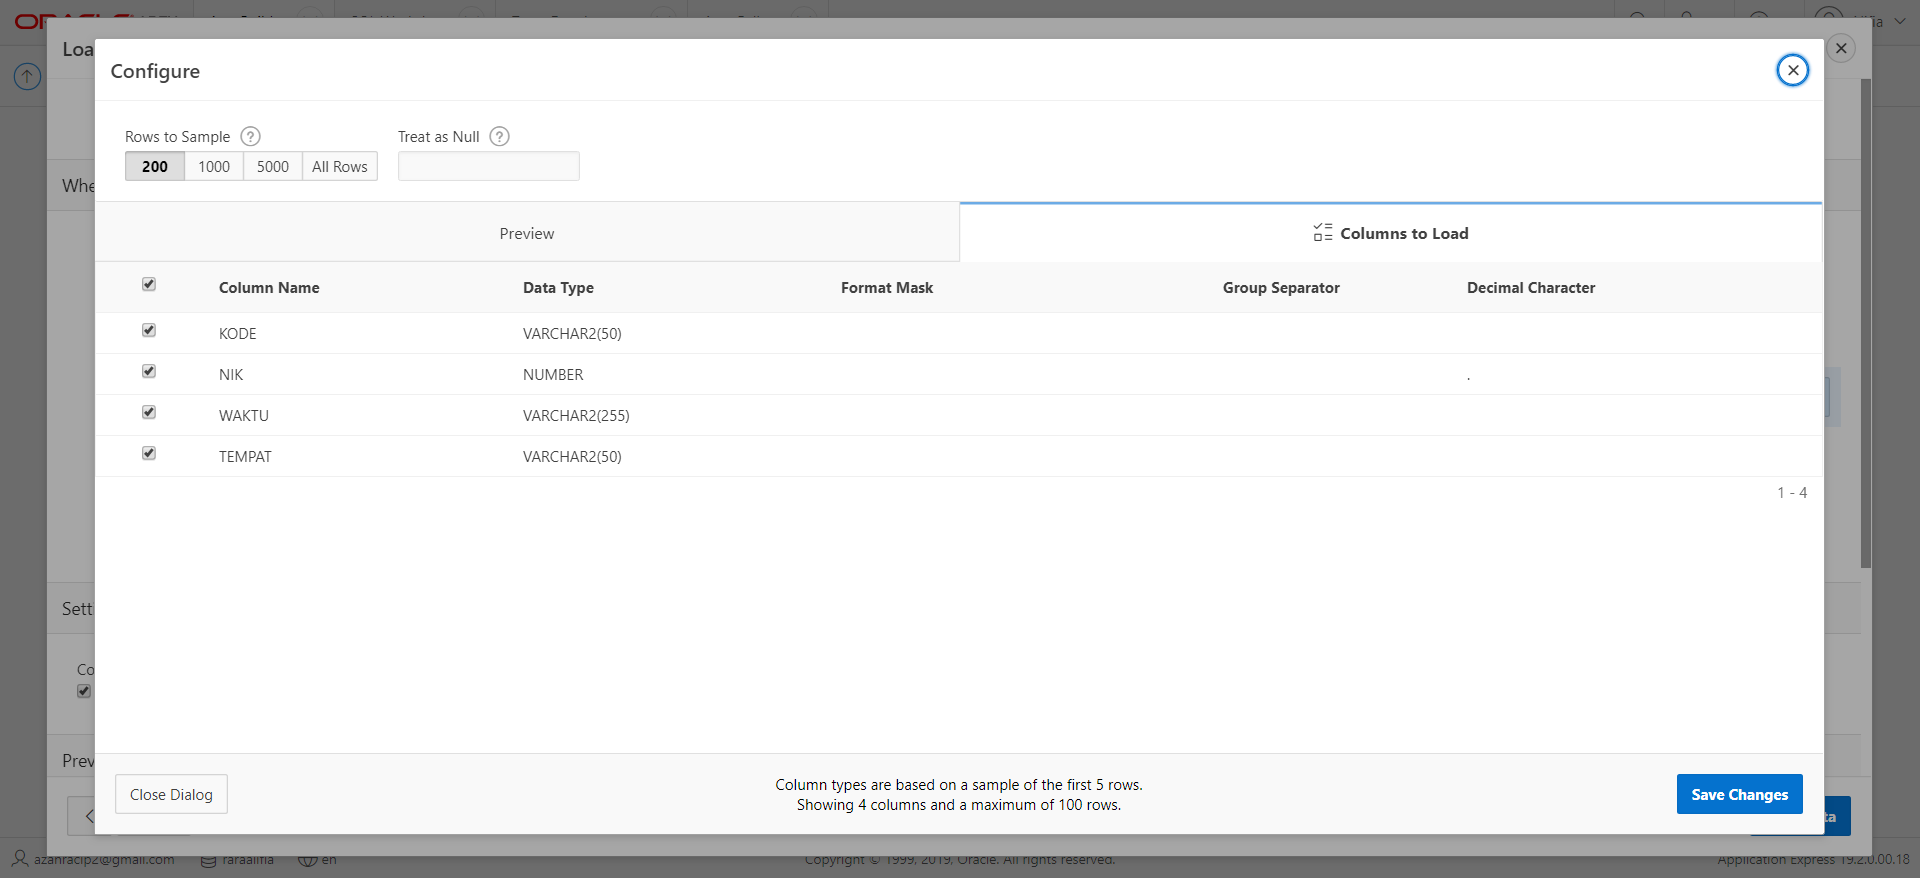
\includegraphics[width=8cm]{Figures/configjadwal.PNG}}
    \item Klik SQL Workshop dan pilih Object Browser, tabel sudah berhasil dibuat. 
         \begin{figure}[h]
        \centerline{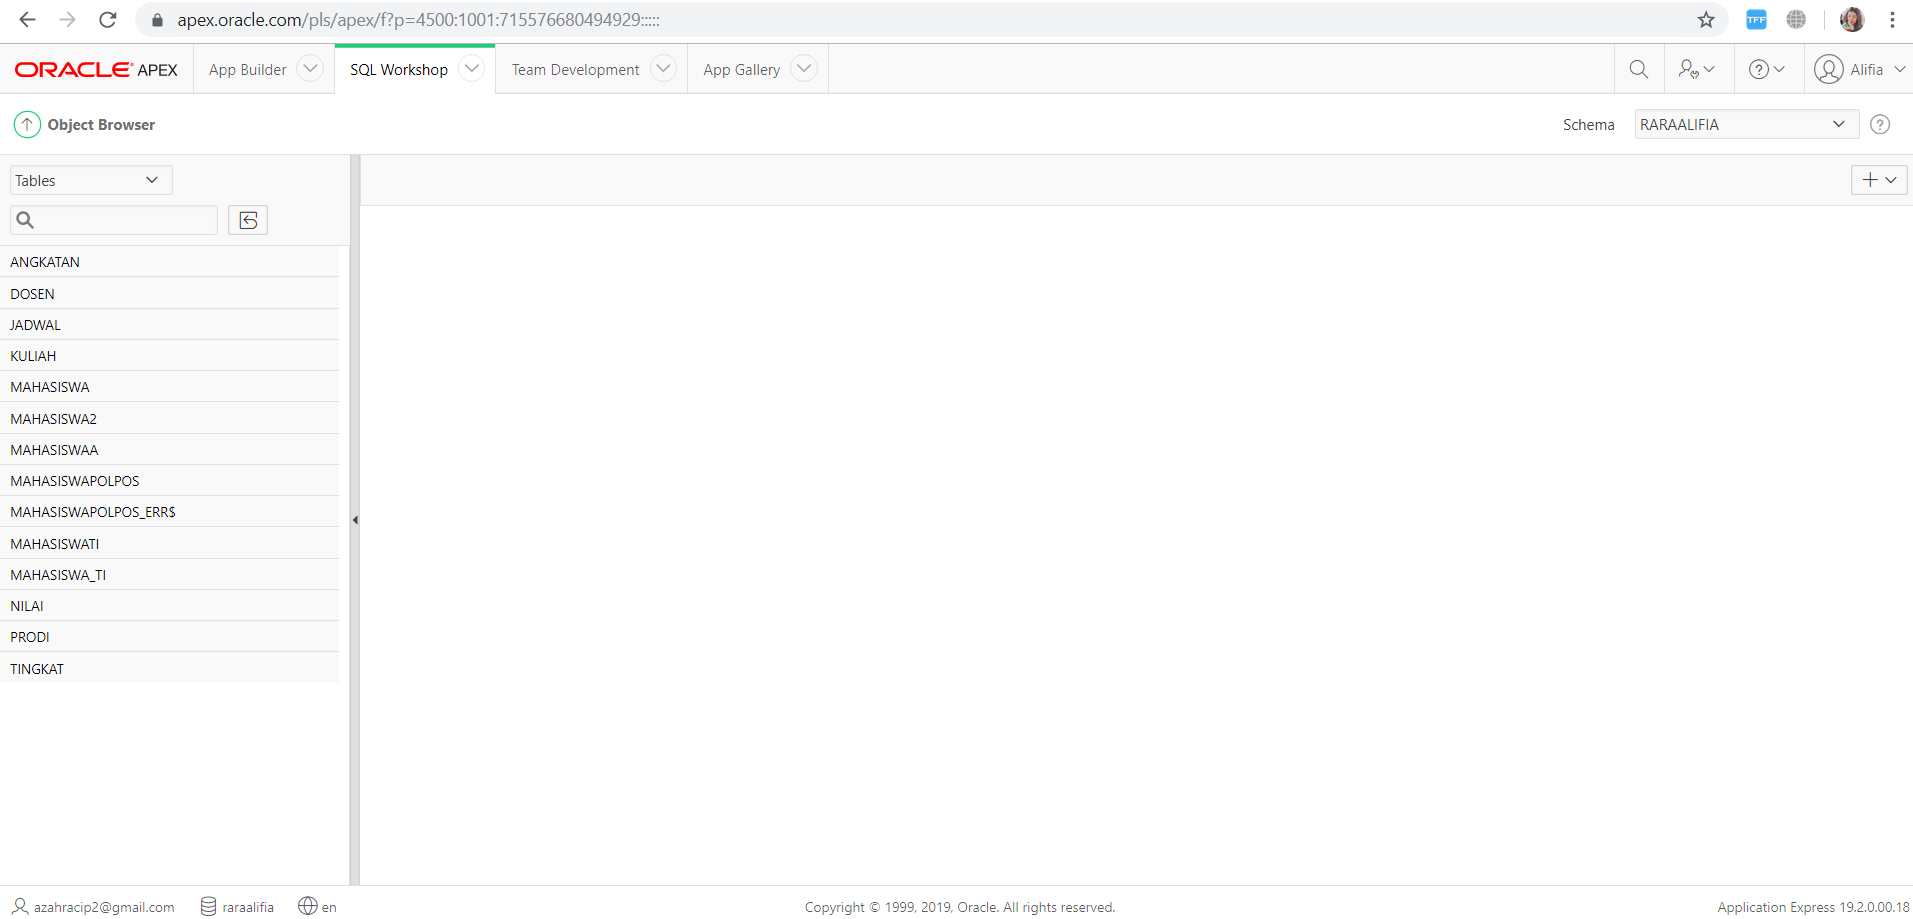
\includegraphics[width=8cm]{Figures/tabelalreadymade.PNG}}
        \end{figure}
    \item Klik satu persatu tabel, hapus atribut id di setiap tabel. Pilih drop column, lalu pilih column id.
        \begin{figure}[h]
        \centerline{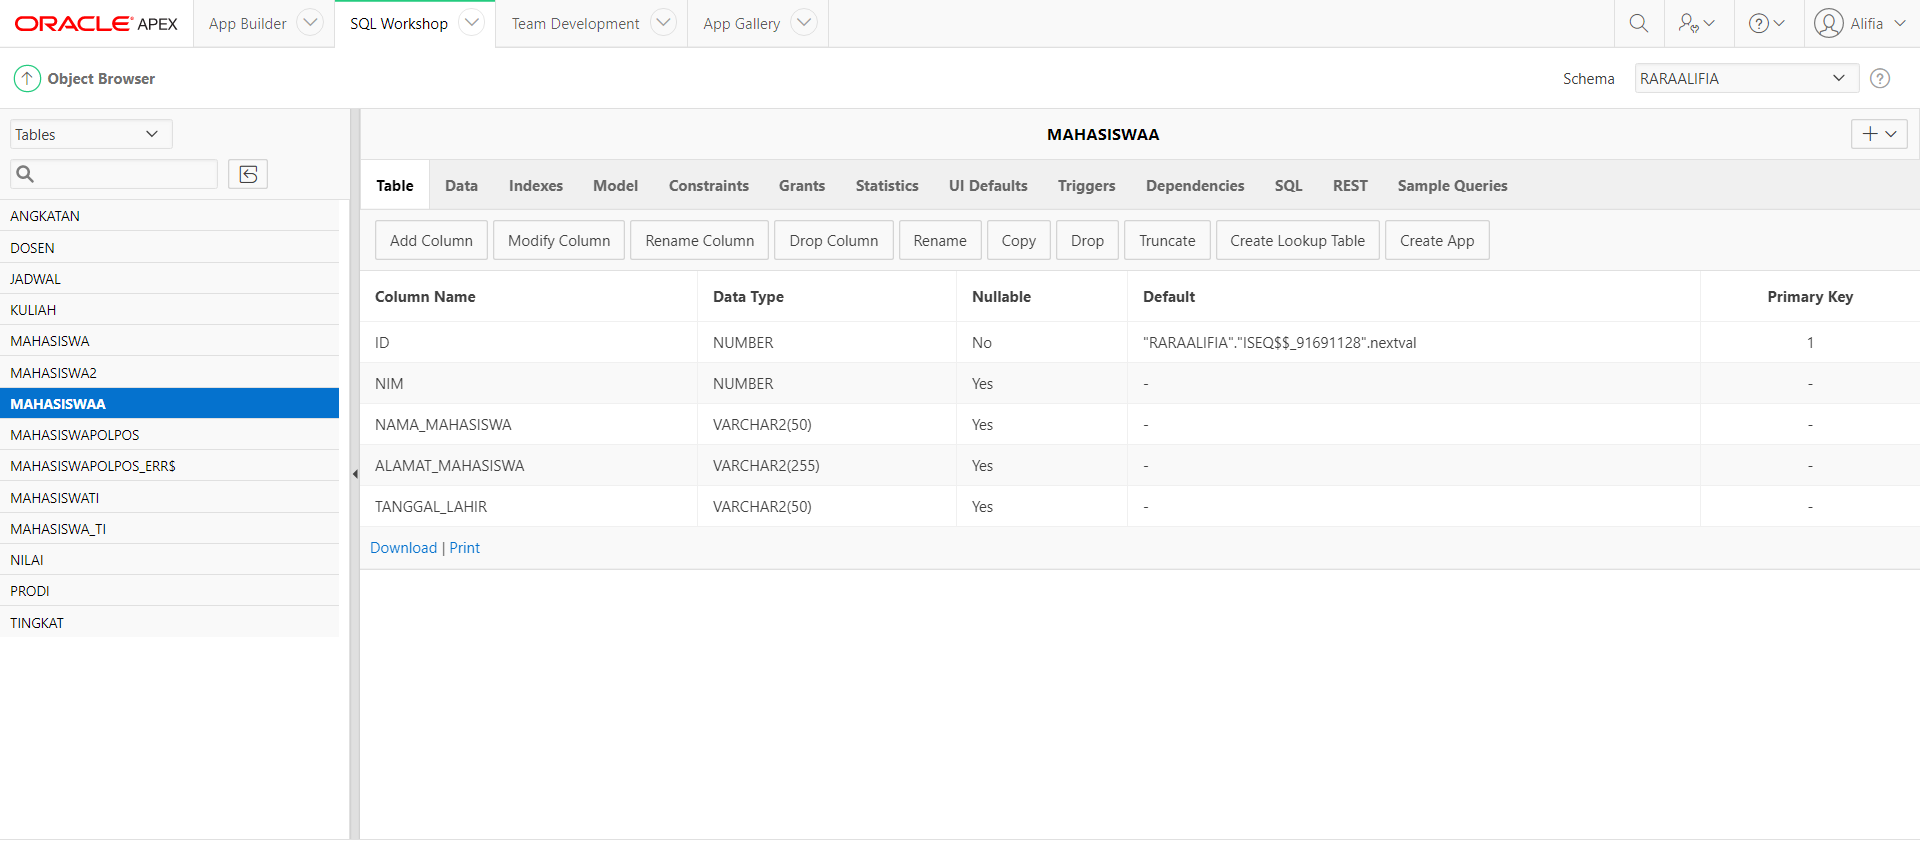
\includegraphics[width=8cm]{Figures/id1.PNG}}
        \end{figure}
        \begin{figure}[h]
        \centerline{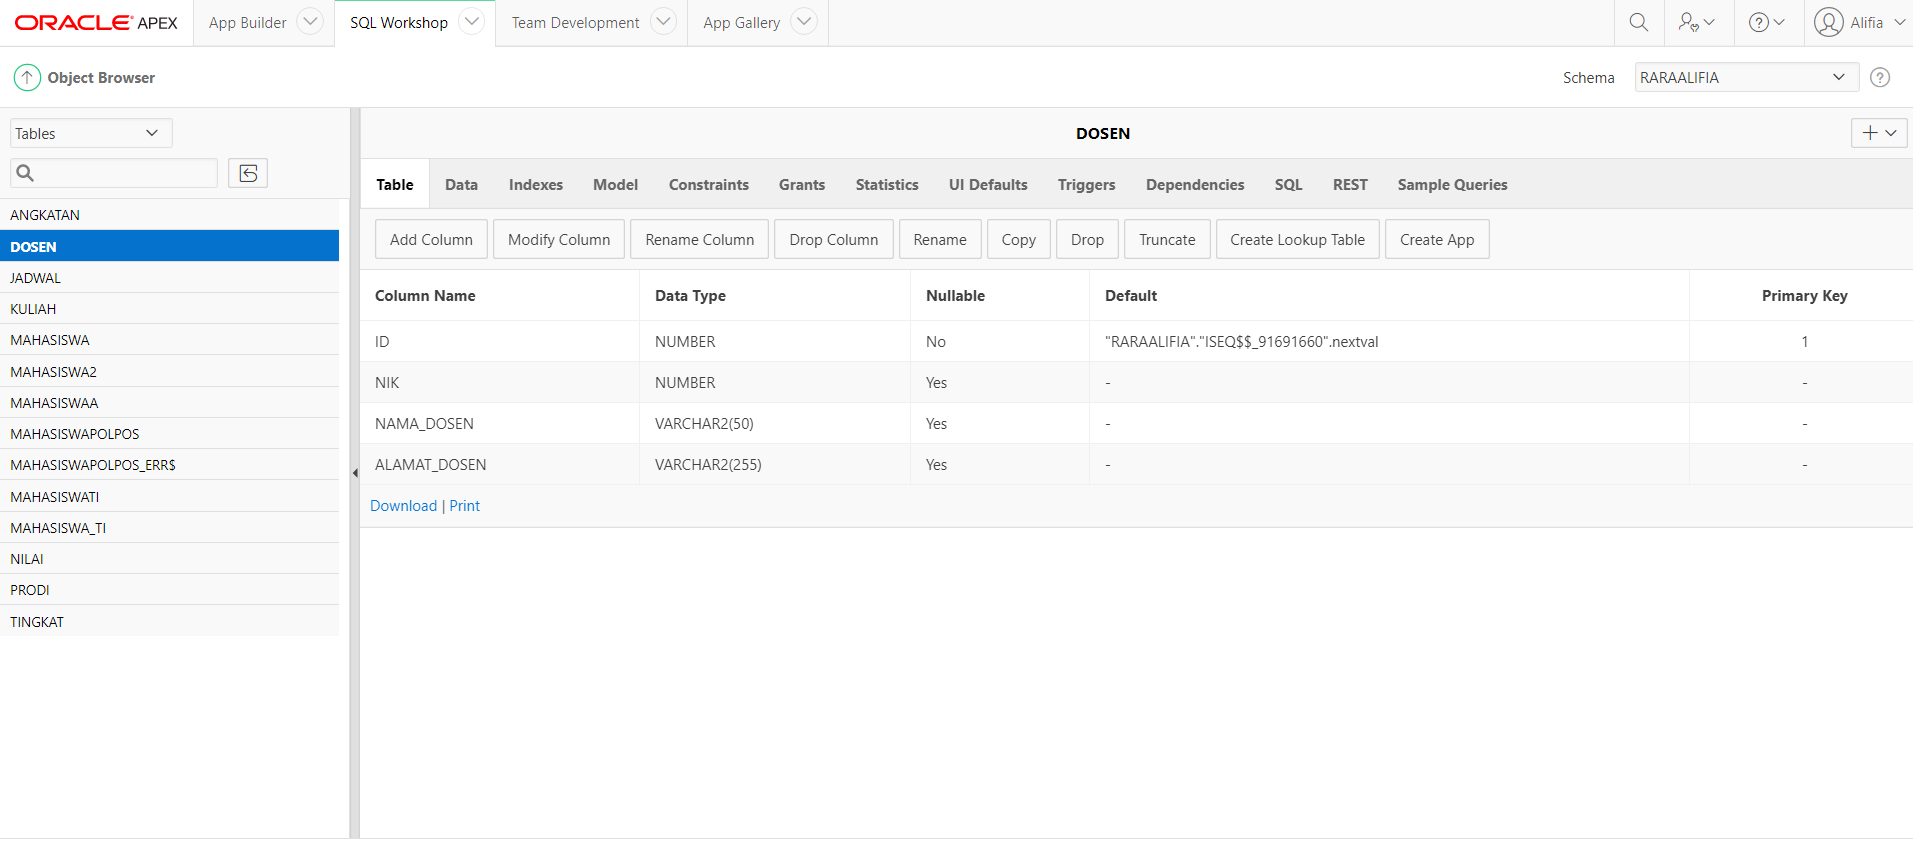
\includegraphics[width=8cm]{Figures/id2.PNG}}
        \end{figure}
        \paragraph{}
        \centerline{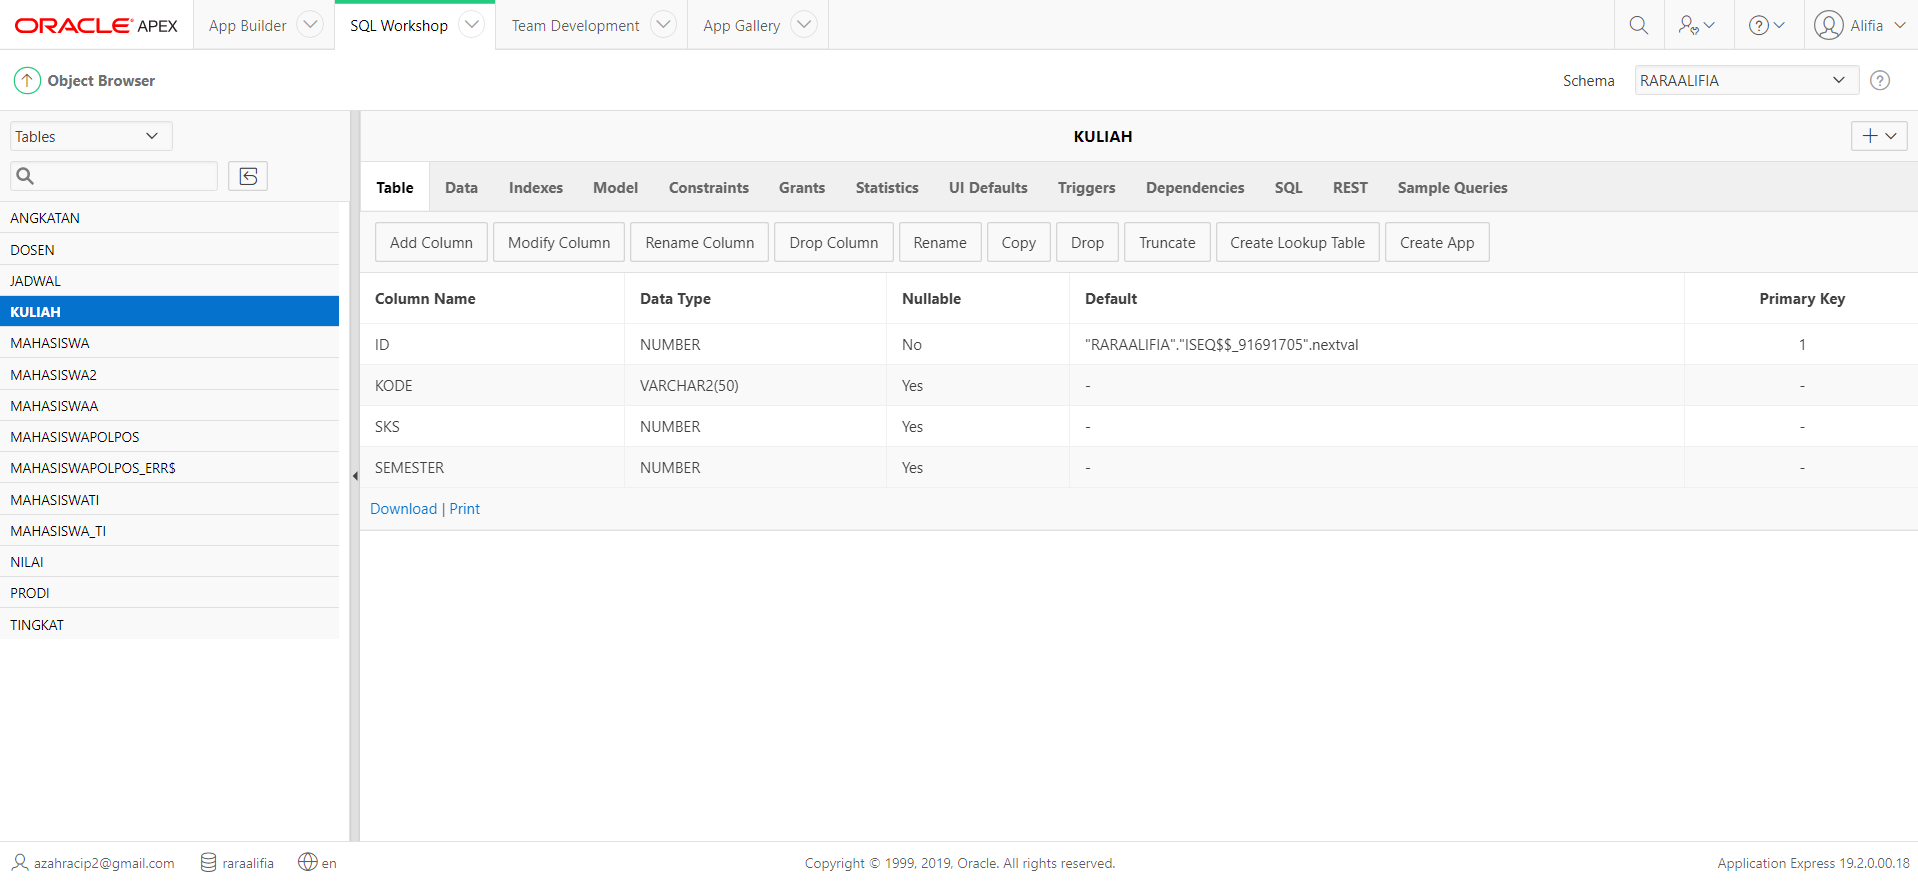
\includegraphics[width=8cm]{Figures/id3.PNG}}
        \paragraph{}
        \centerline{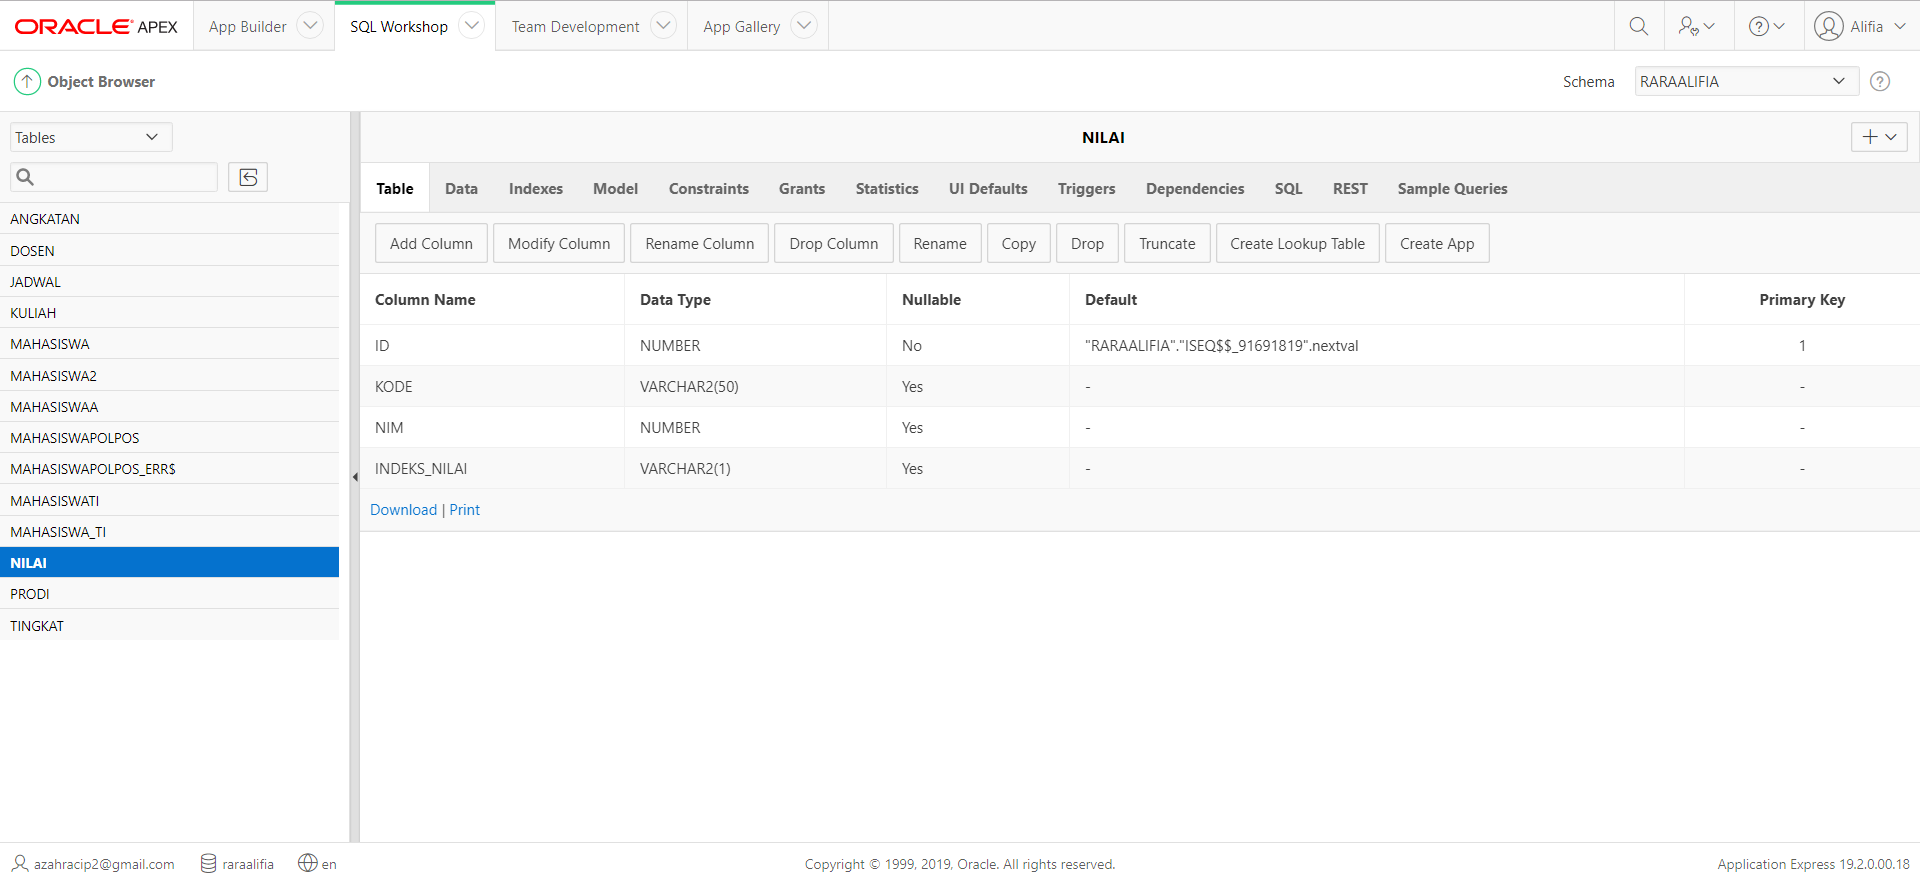
\includegraphics[width=8cm]{Figures/id4.PNG}}
        \begin{figure}[h]
        \centerline{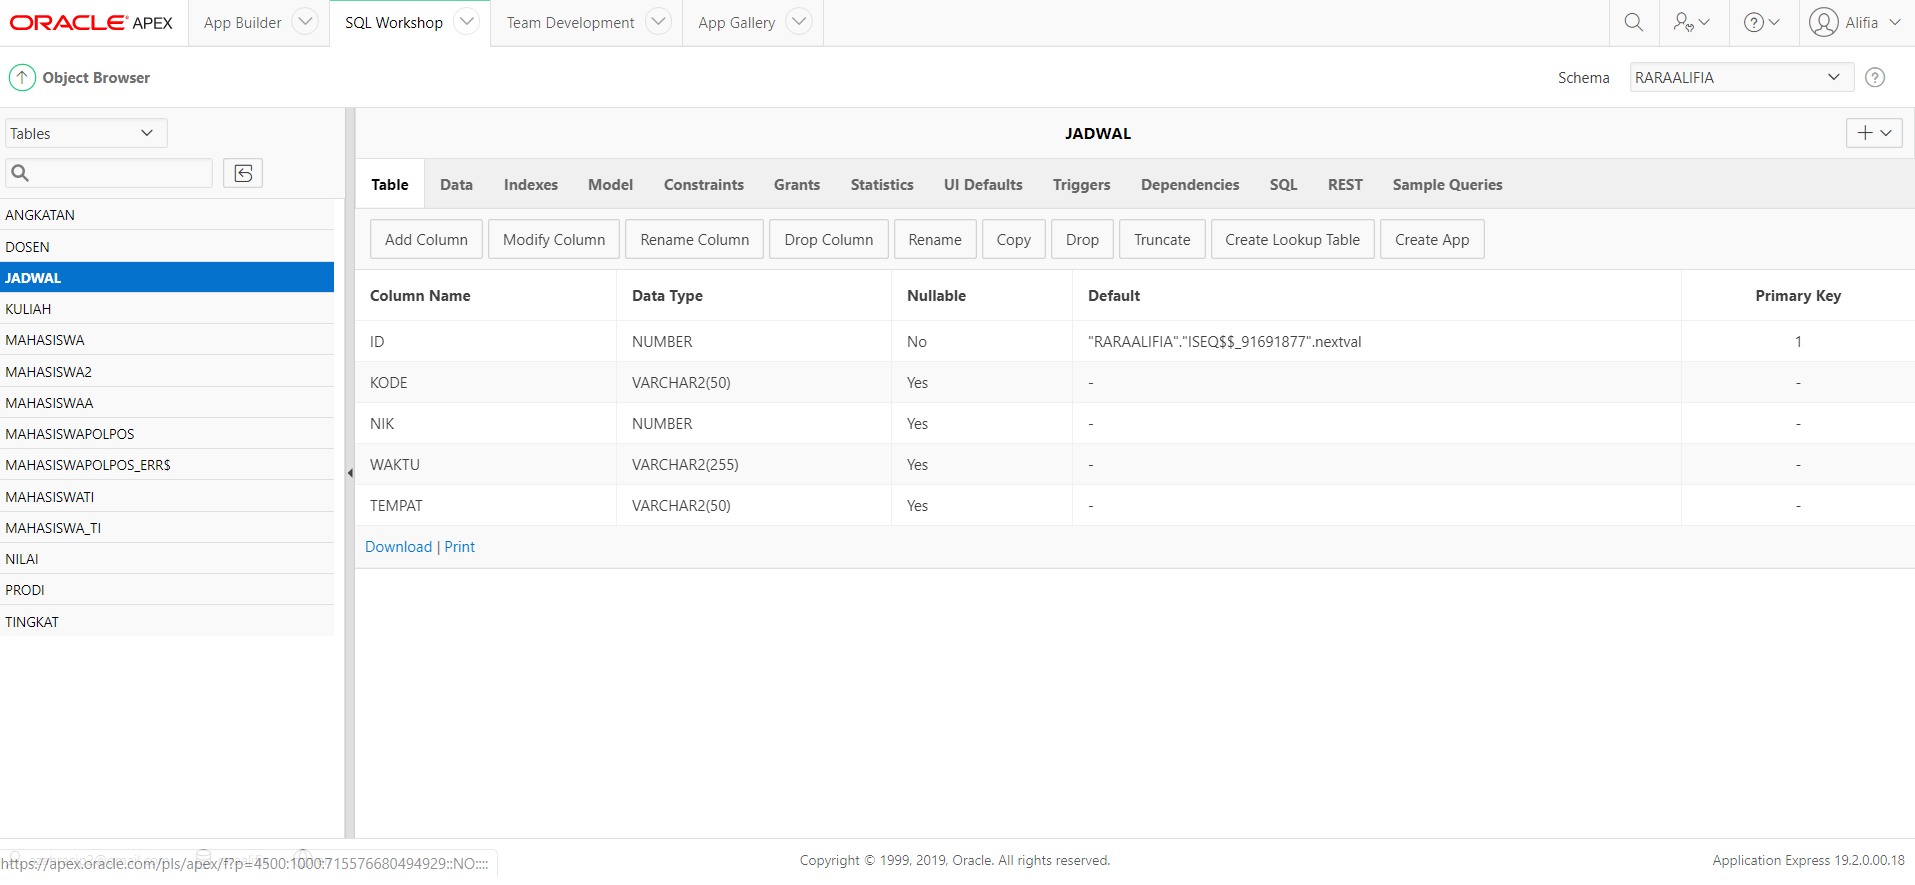
\includegraphics[width=8cm]{Figures/id5.PNG}}
        \end{figure}
    \item Pilih Tabel Mahasiswaa lalu klik Constrains klik create dan jadikan NIM Sebagai Primary Key, Lalu Next. 
        \begin{figure}[h]
        \centerline{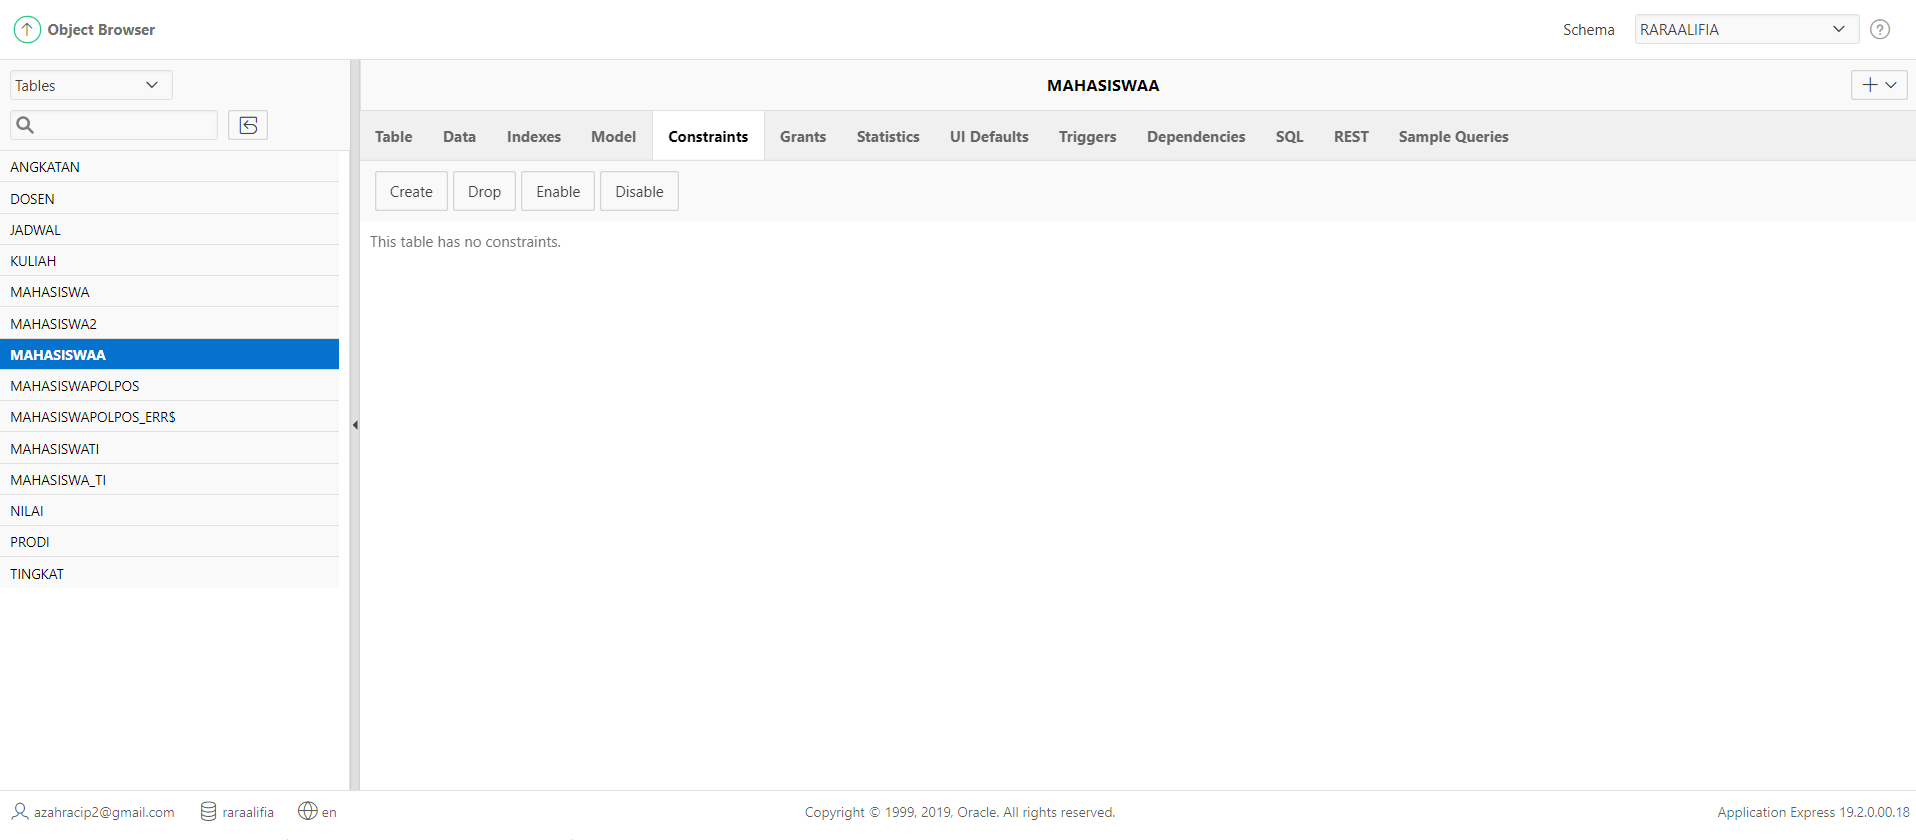
\includegraphics[width=8cm]{Figures/constraintmahasiswa.PNG}}
        \end{figure}
    \item Pilih Tabel Dosen lalu klik Constrains klik create dan jadikan NIM Sebagai Primary Key, Lalu Next. 
        \begin{figure}[h]
        \centerline{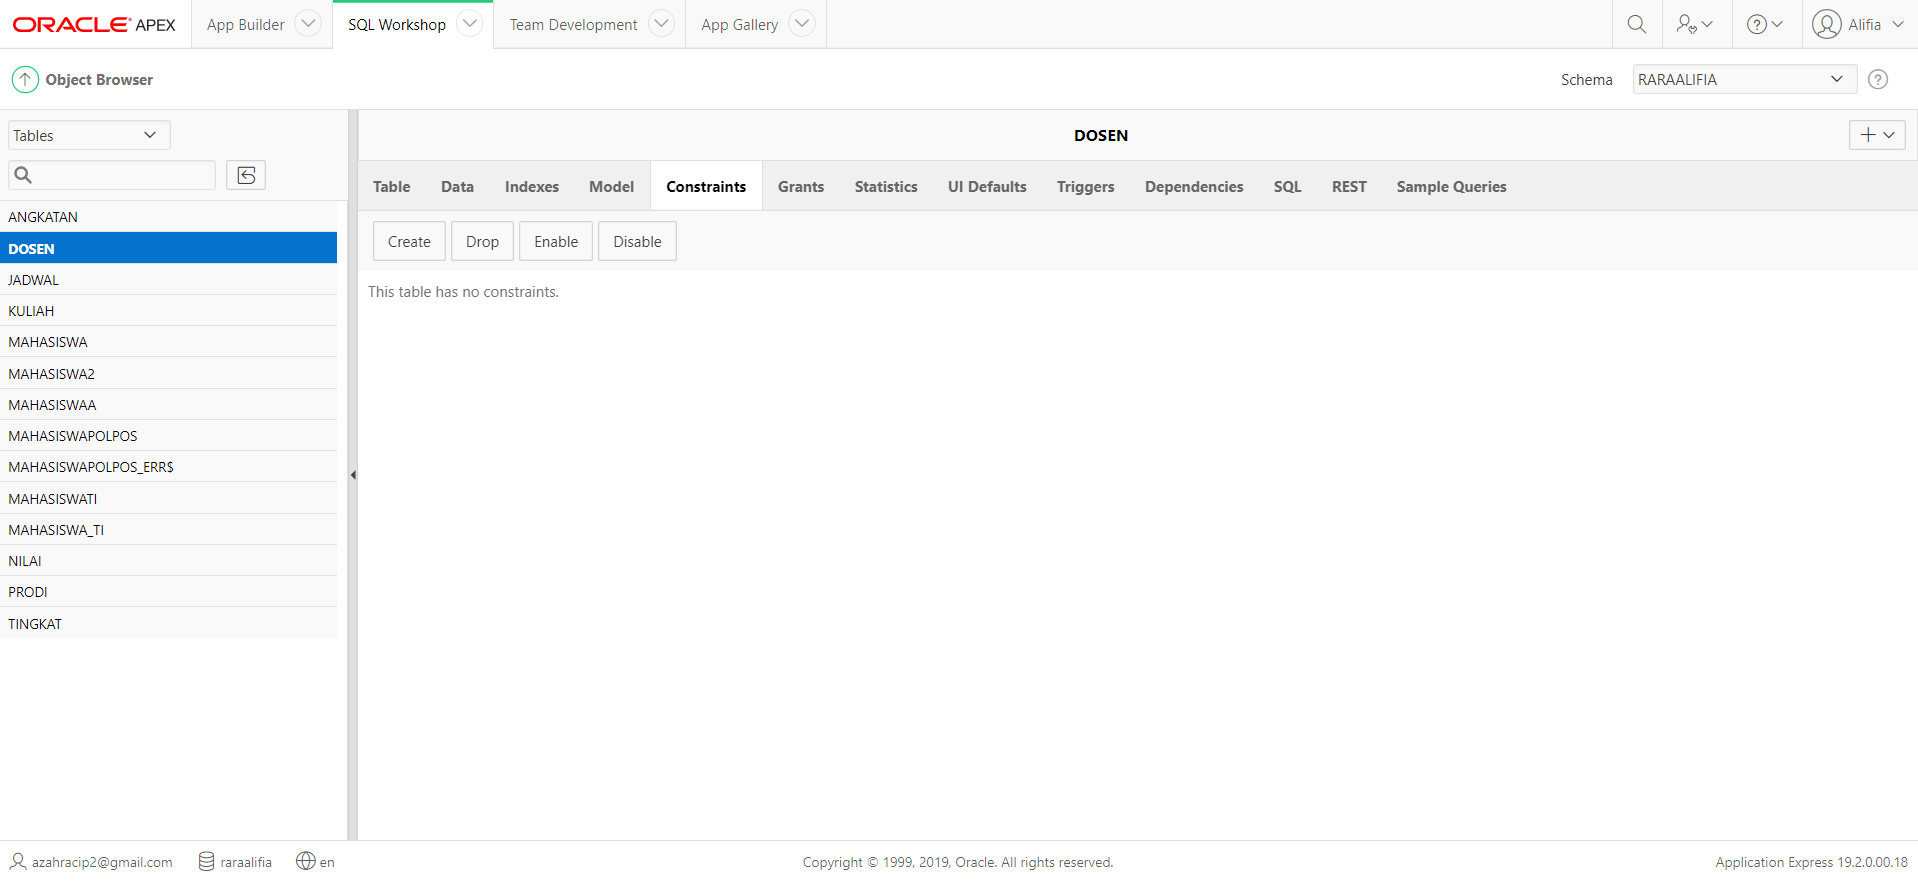
\includegraphics[width=8cm]{Figures/constraintdosen.PNG}}
        \end{figure}
     \item Pilih Tabel Kuliah lalu klik Constrains klik create dan jadikan Kode Sebagai Primary Key, Lalu Next.
     \item Pilih Tabel Jadwal lalu klik Constrains klik create dan pilih foreign key, pindahkan kode ke sebelah kanan dan pilih references table kuliah, pindahkan kode ke sebelah kanan. Next
        \begin{figure}[h]
        \centerline{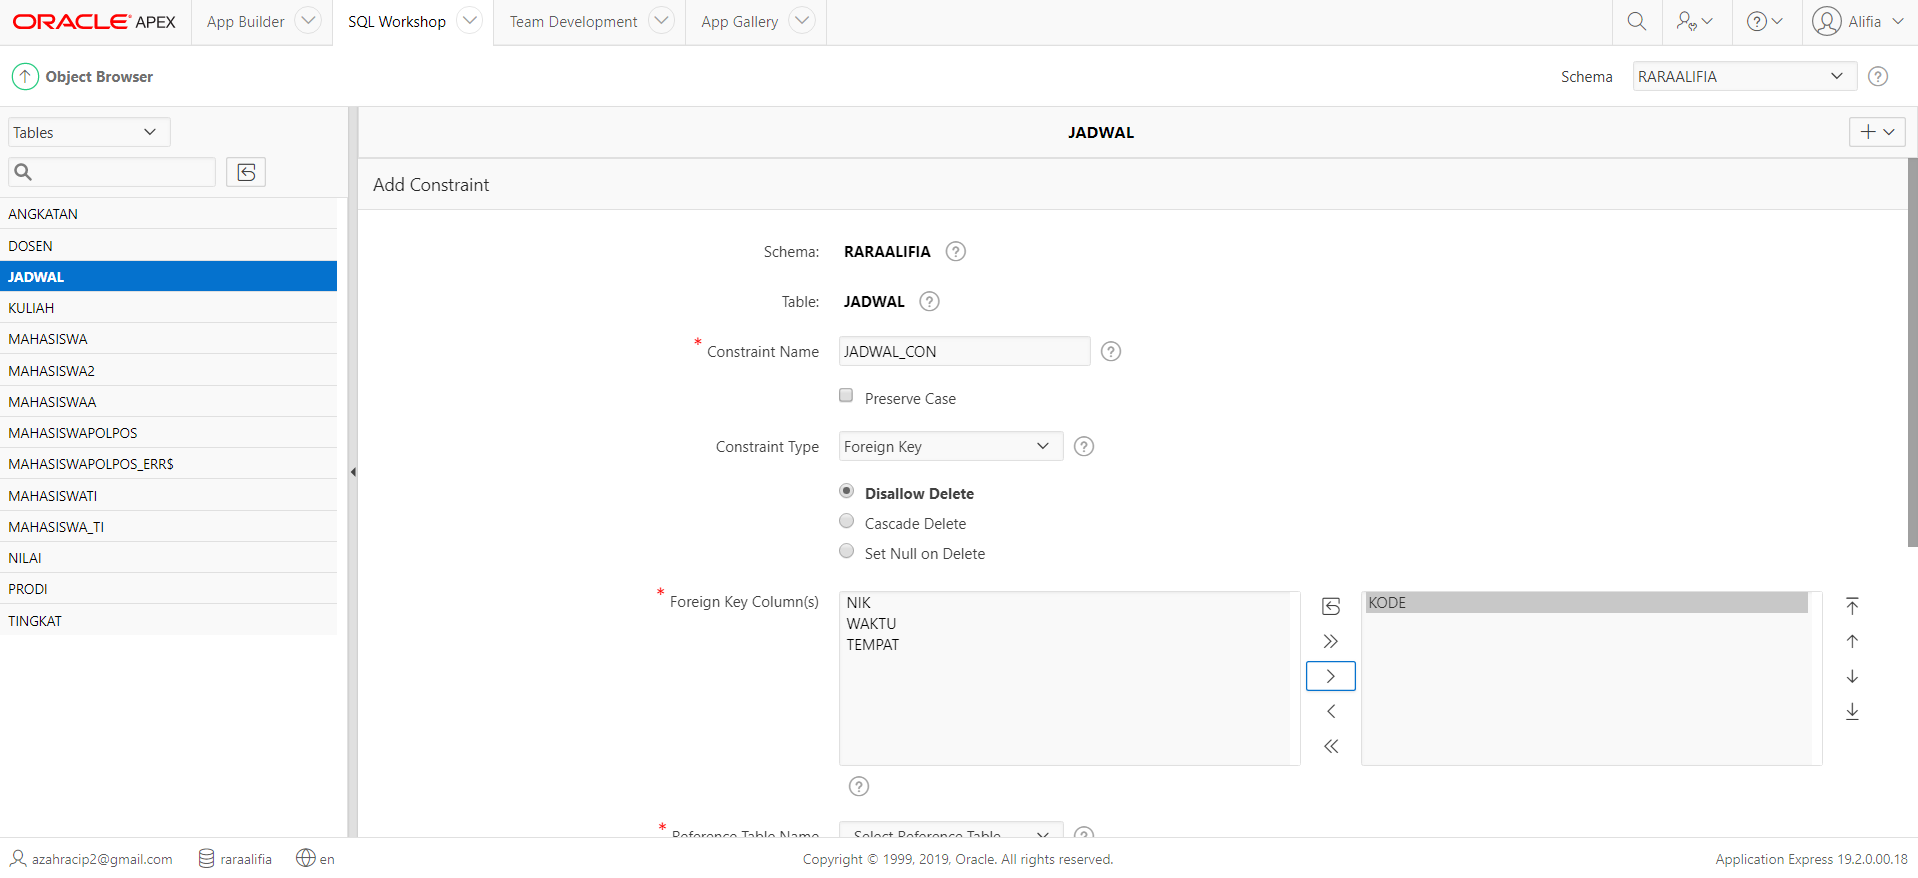
\includegraphics[width=8cm]{Figures/constraintjadwal.PNG}}
        \end{figure}
        \begin{figure}[h]
        \centerline{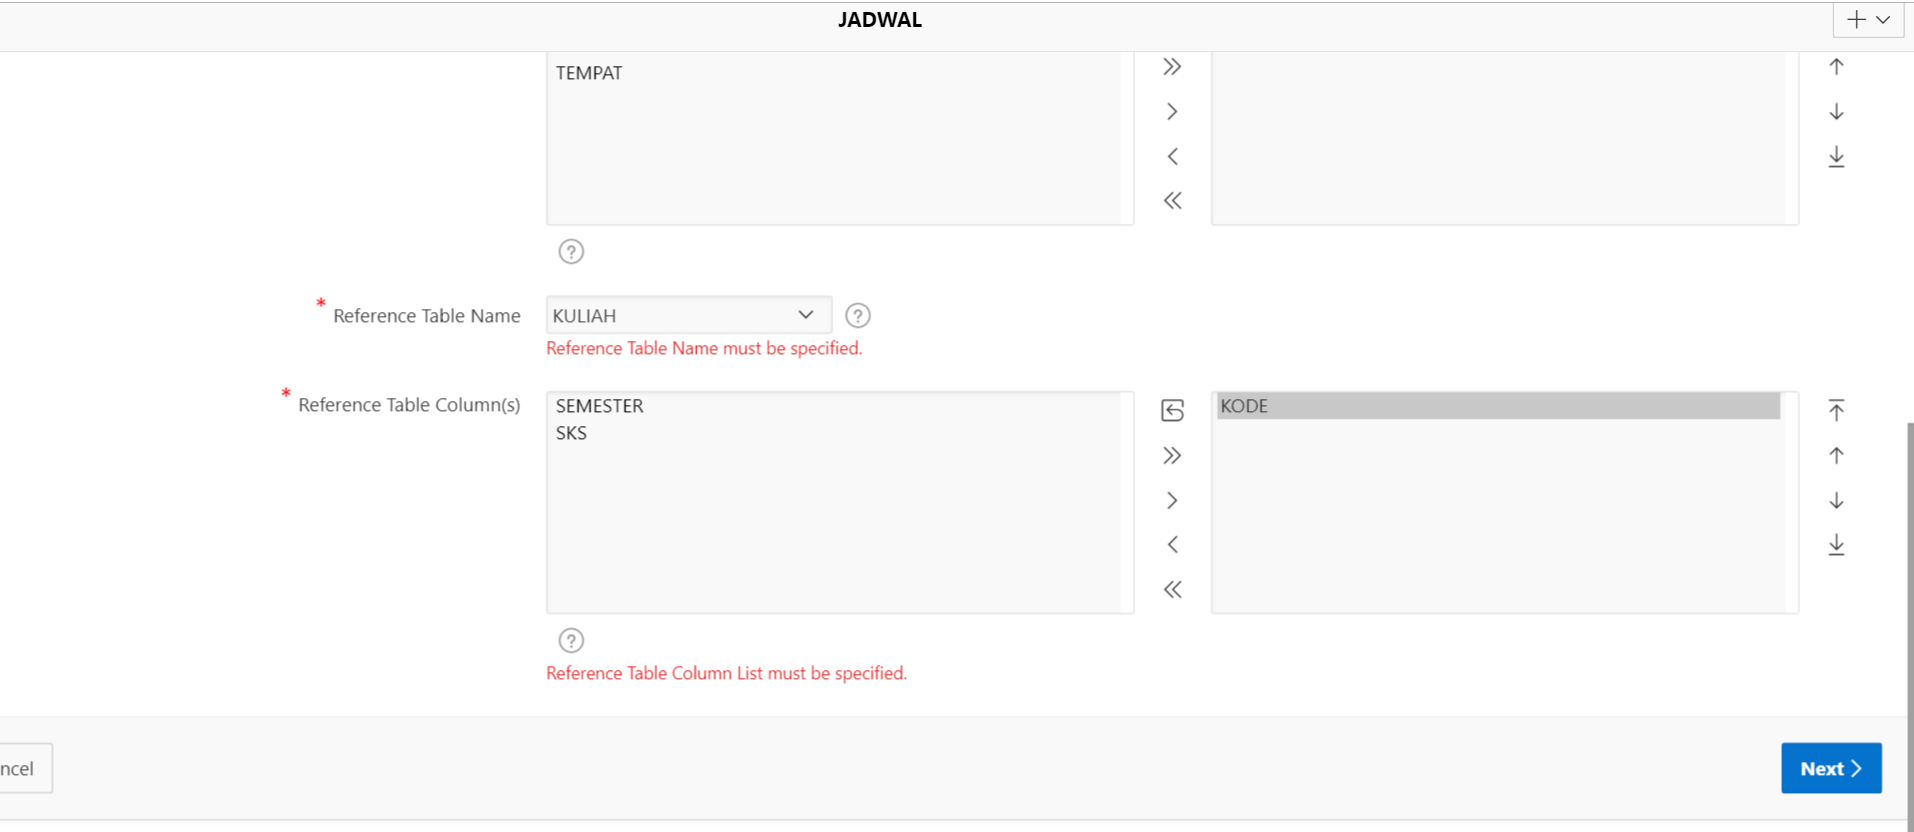
\includegraphics[width=8cm]{Figures/constraintjadwal2.PNG}}
        \end{figure}
    \item Pilih Tabel Nilai lalu klik Constrains klik create dan pilih foreign key, pindahkan kode ke sebelah kanan dan pilih references table kuliah, pindahkan kode ke sebelah kanan. Next
        \begin{figure}[h]
        \centerline{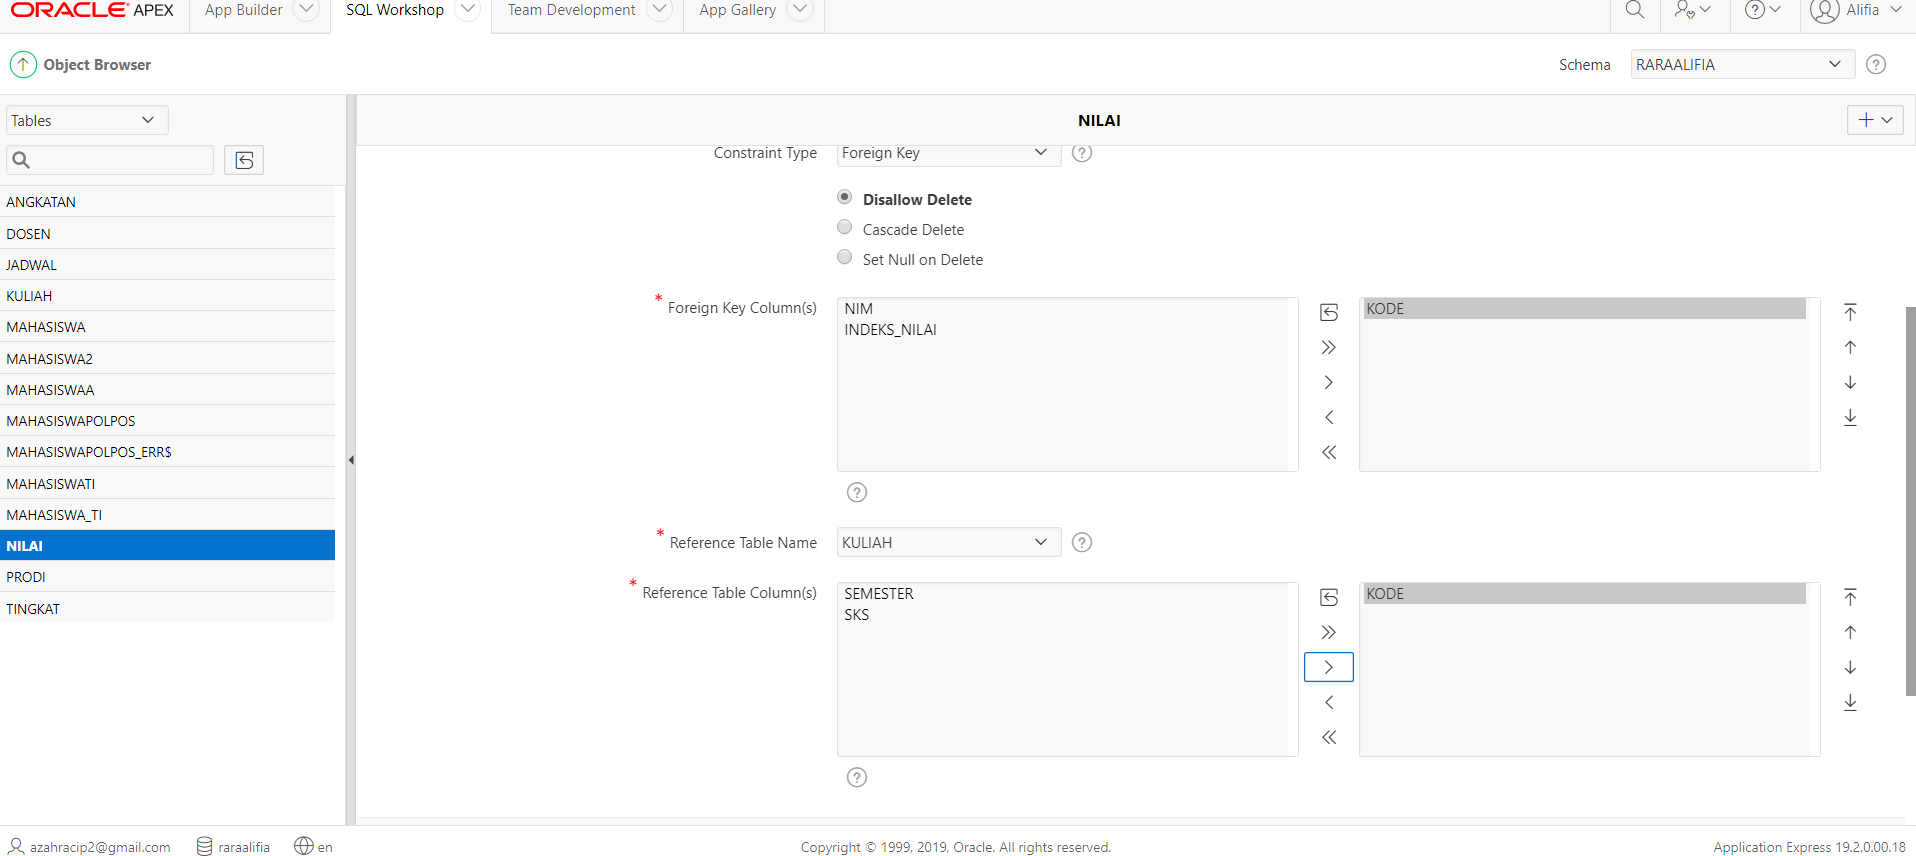
\includegraphics[width=8cm]{Figures/constrainsnilai.PNG}}
        \end{figure}
    \item Pergi ke app builder kemudian klik create.
        \paragraph{}
        \centerline{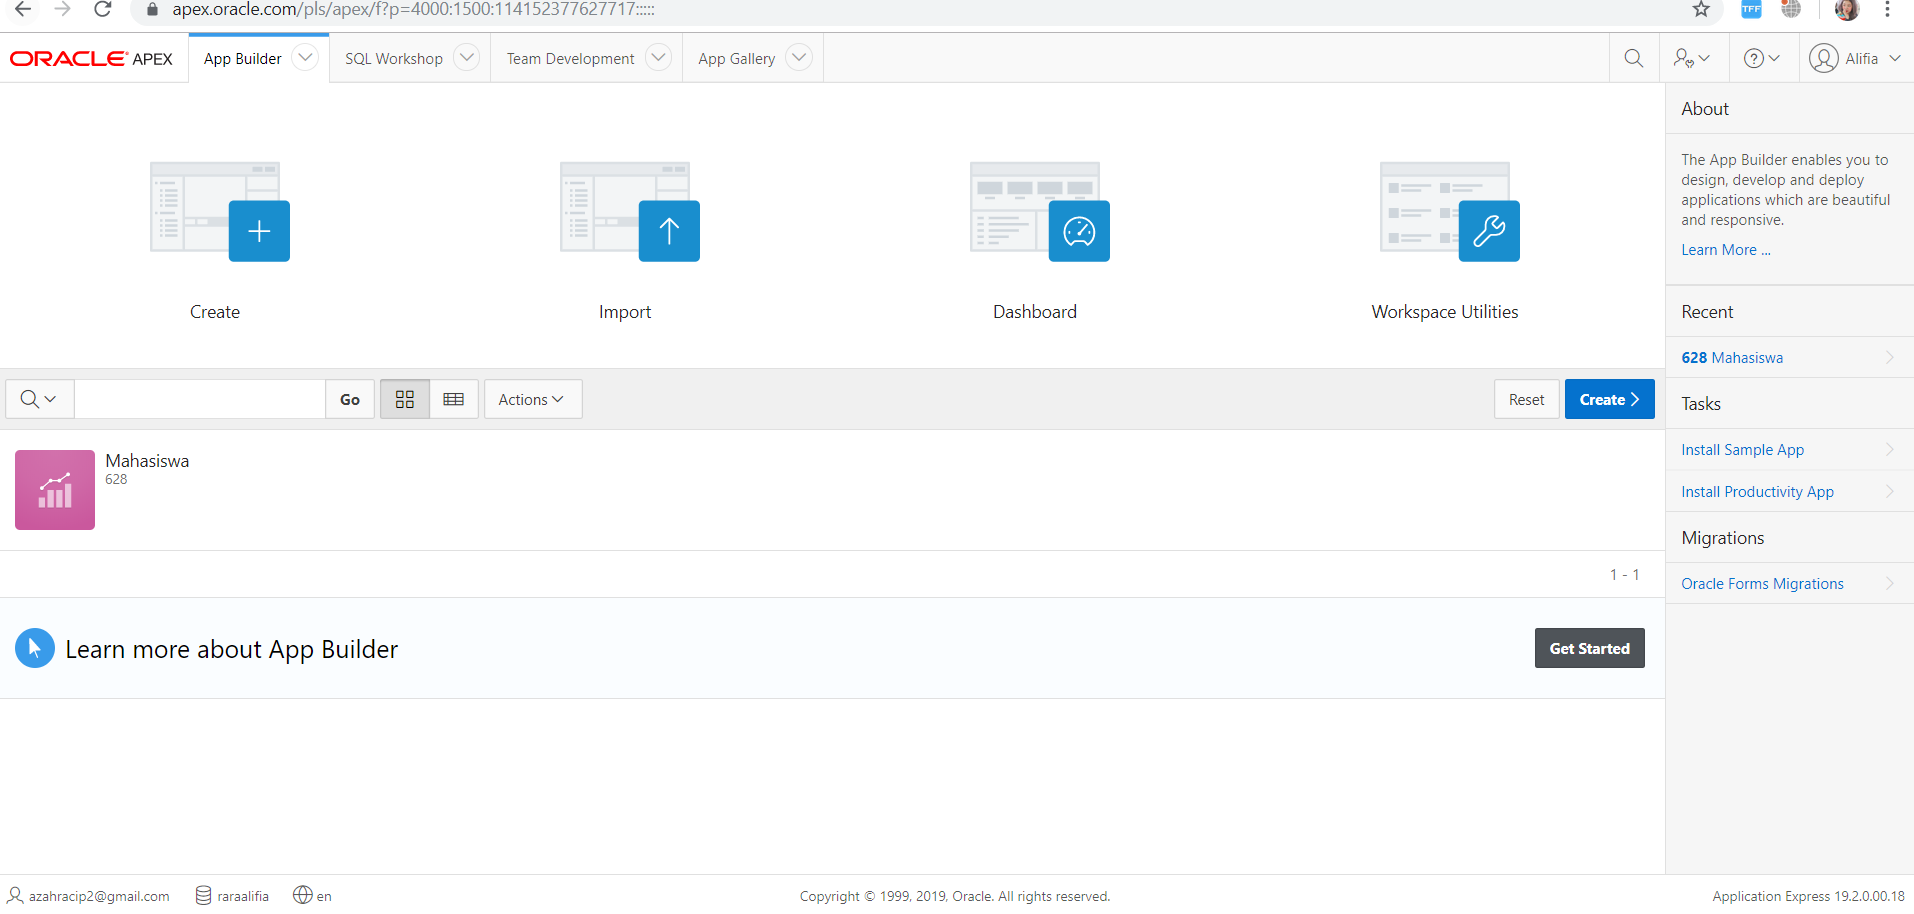
\includegraphics[width=8cm]{GAMBAR/CREATE.PNG}}
    \item Klik new application untuk membuat aplikasi baru
        \begin{figure}[h]
        \centerline{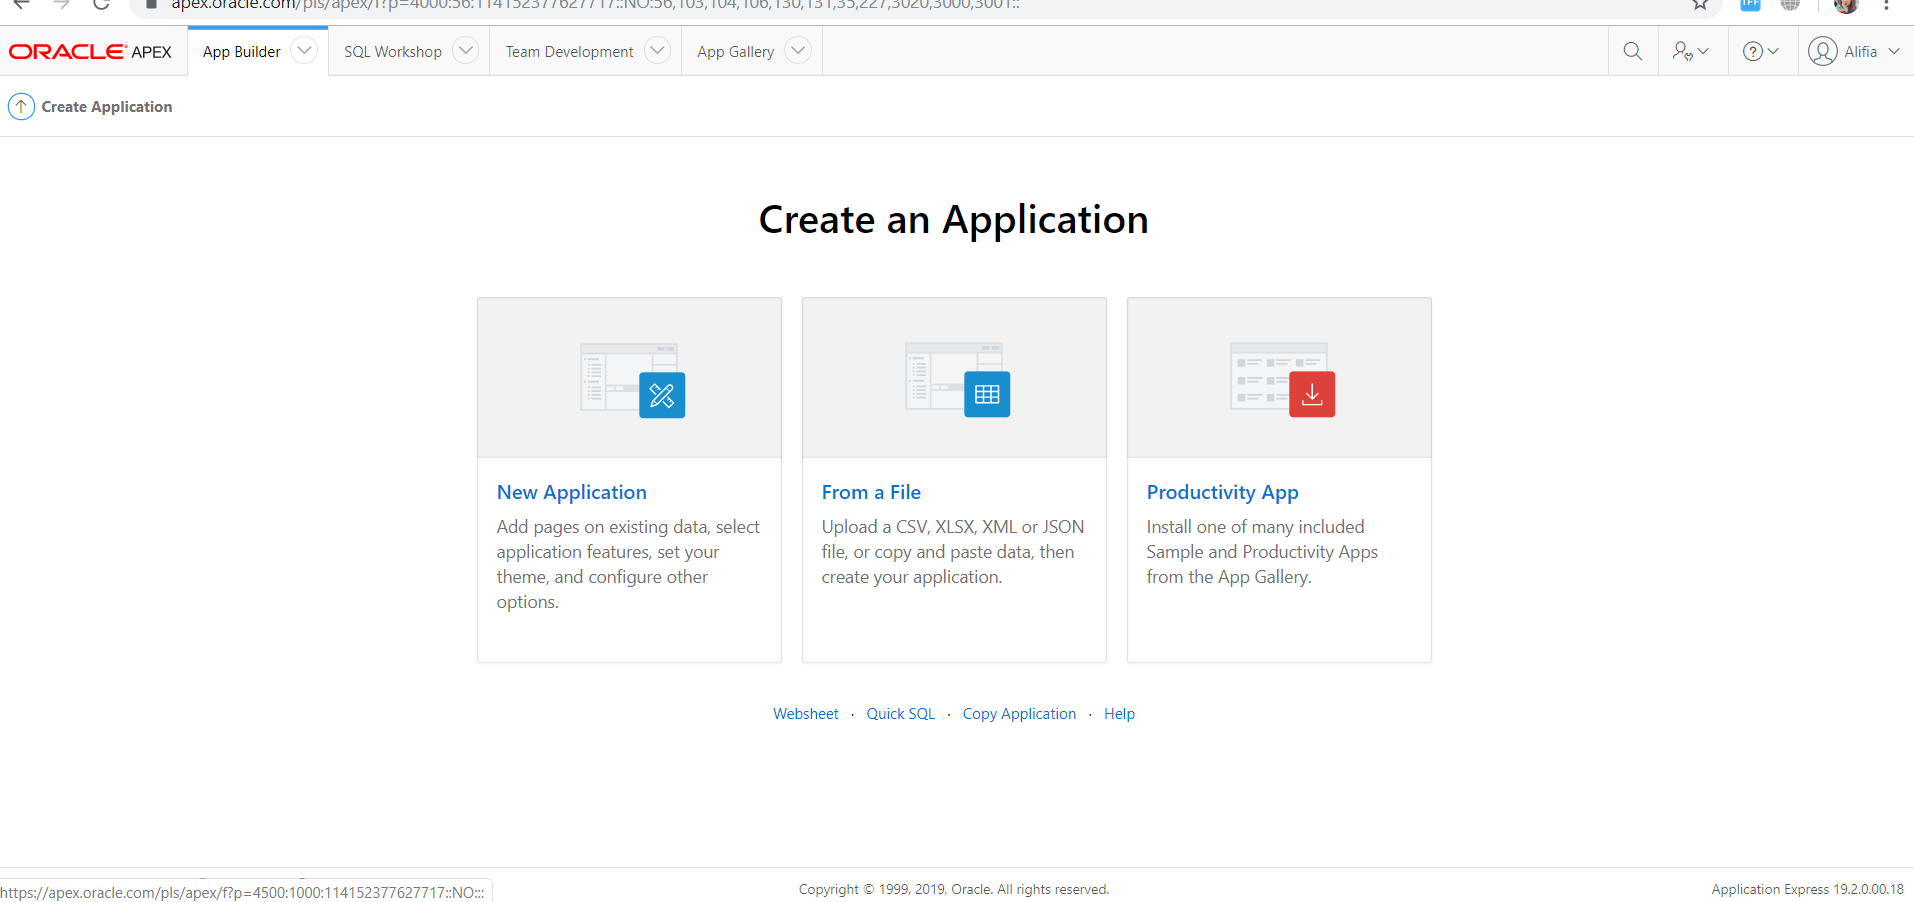
\includegraphics[width=8cm]{GAMBAR/NEWAPP.PNG}}
        \end{figure}
    \item Isi nama aplikasi sesuai keinginan anda
        \paragraph{}
        \centerline{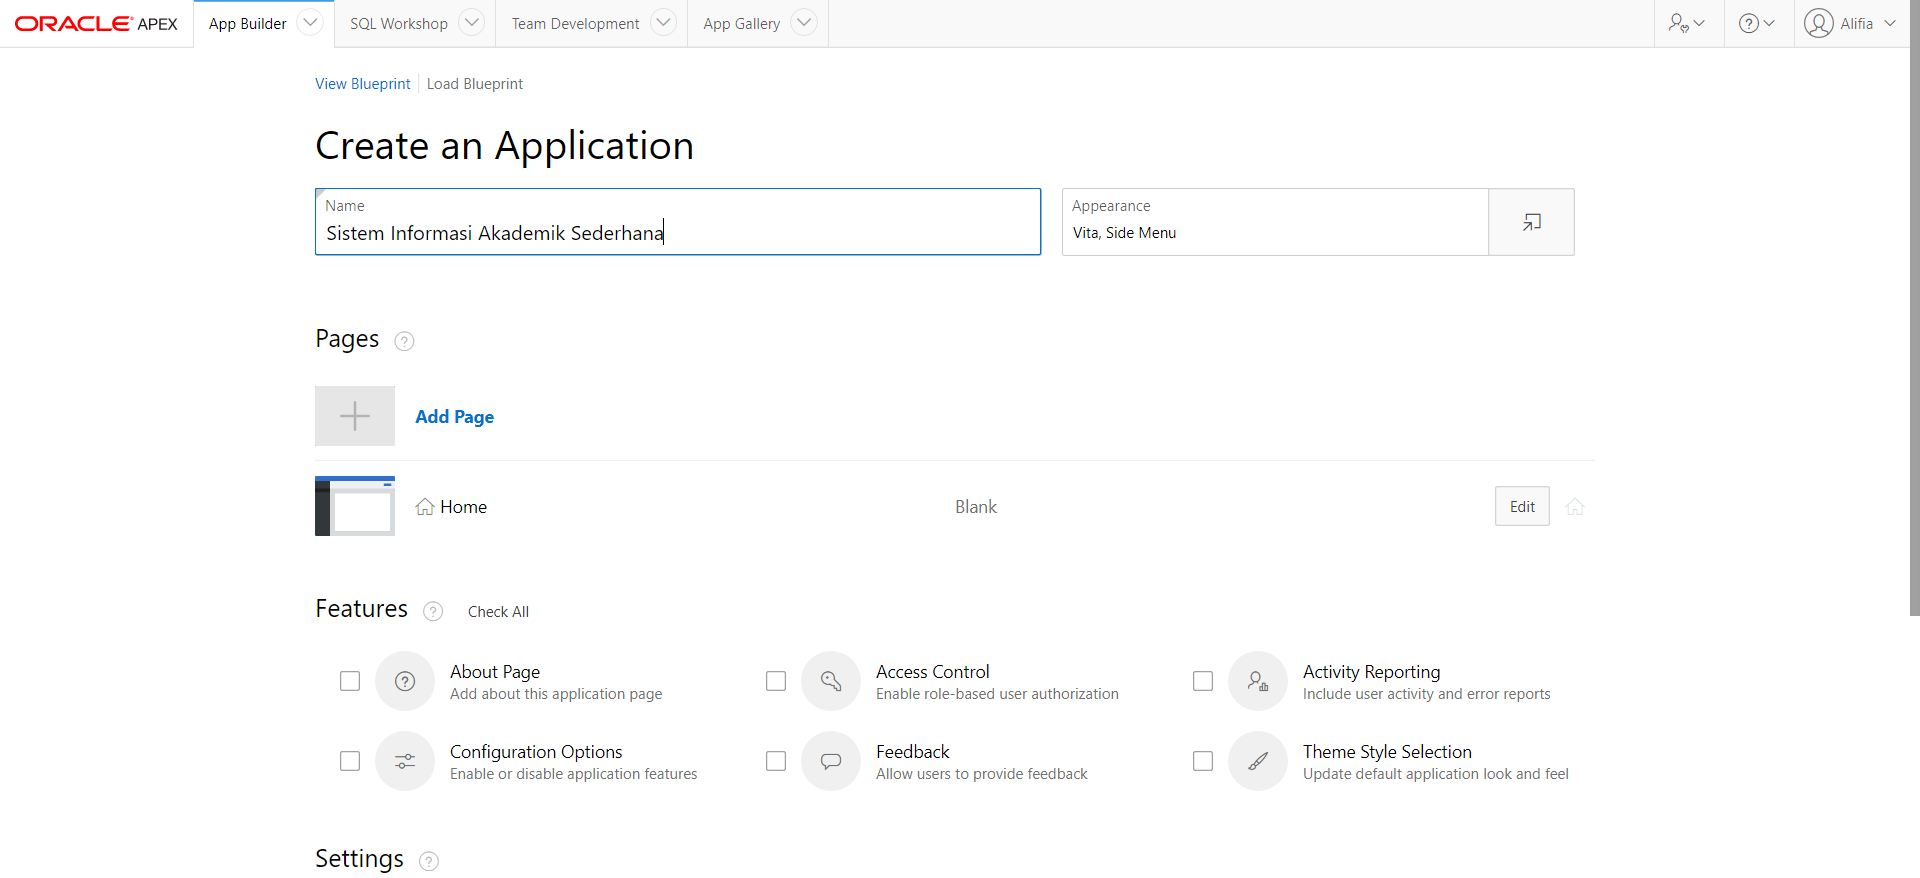
\includegraphics[width=8cm]{Figures/namaaplikasi.PNG}}
    \item Langkah selanjutnya add page, kemudian pilih interactive report. Isi table name sesuai urutan tabel, tabel mahasiswa.
        \paragraph{}
        \centerline{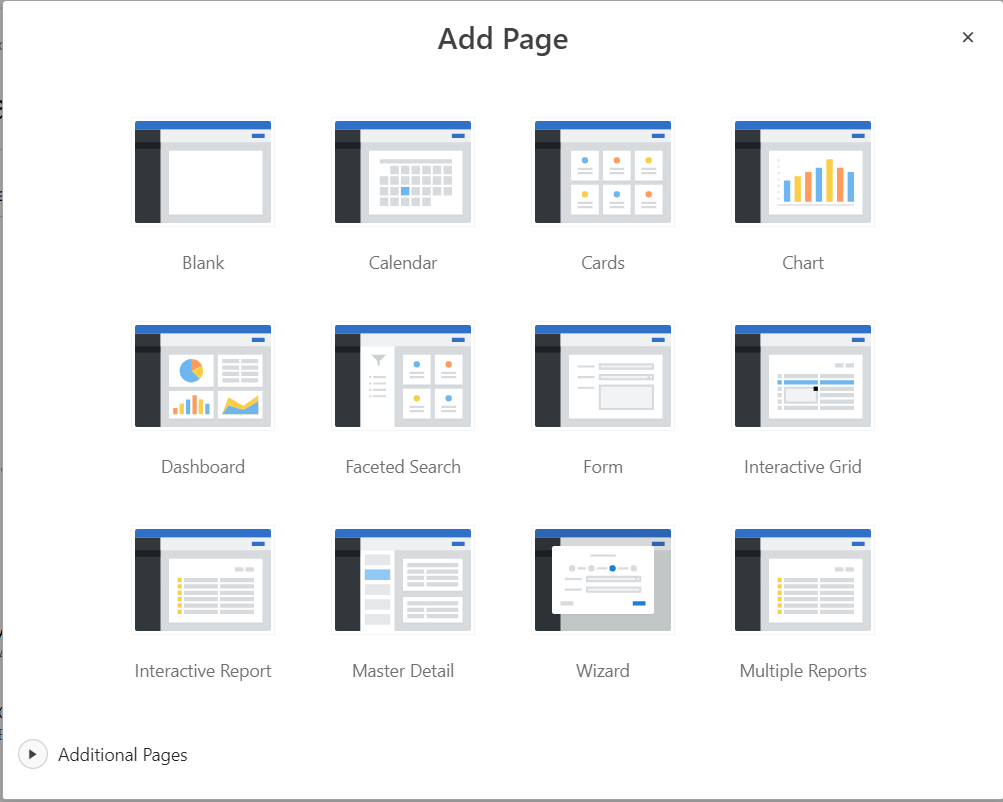
\includegraphics[width=8cm]{Figures/interactivereport.PNG}}
        \begin{figure}[h]
        \centerline{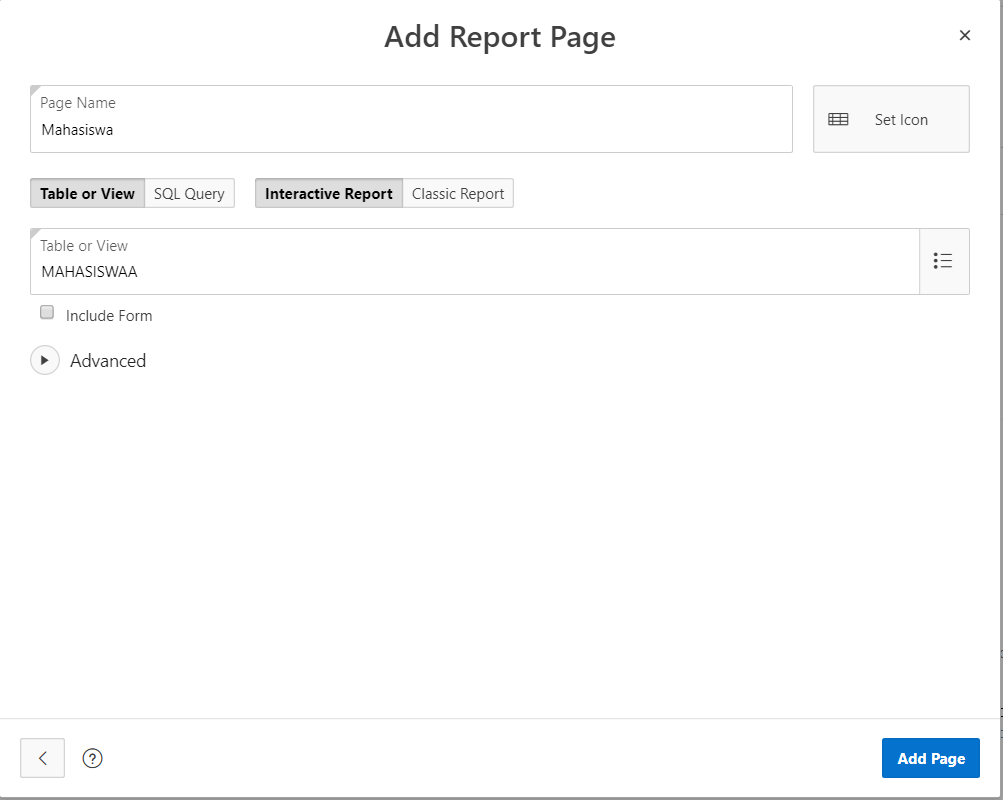
\includegraphics[width=8cm]{Figures/Addpage.PNG}}
        \end{figure}
    \item Lalu pilih add page kembali kemudian pilih interactive report. Isi table name sesuai urutan tabel, tabel dosen.
        \begin{figure}[h]
        \centerline{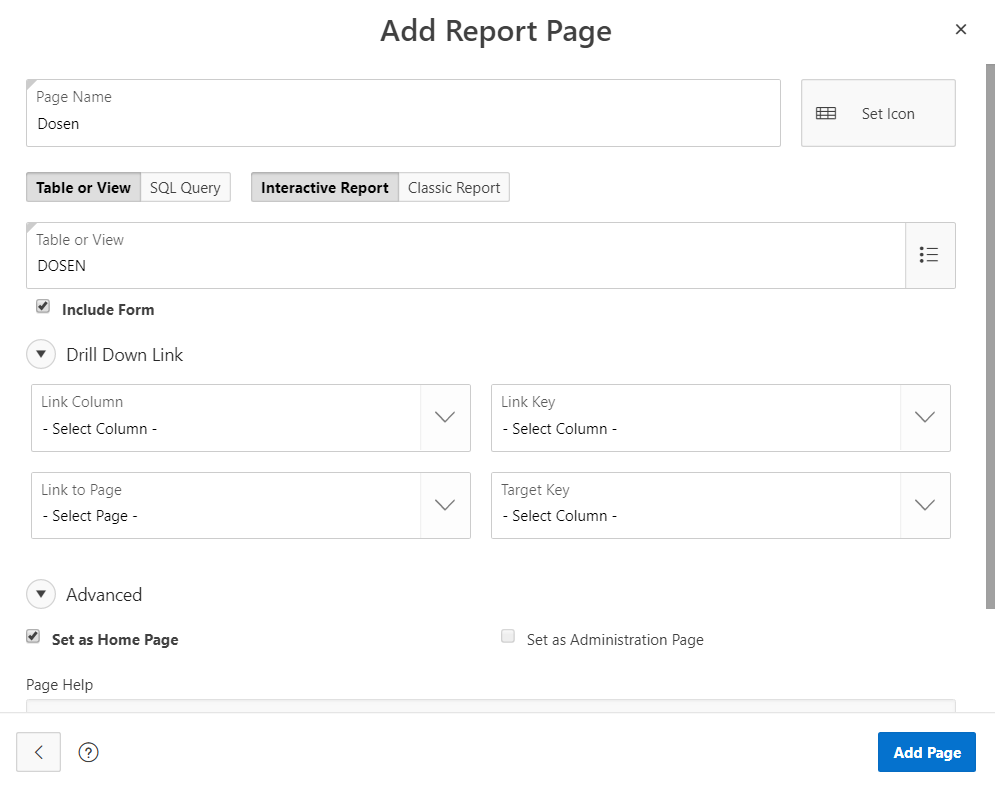
\includegraphics[width=8cm]{Figures/addpagedosen.PNG}}
        \end{figure}
    \item Lalu pilih add page kembali kemudian pilih interactive report. Isi table name sesuai urutan tabel, tabel kuliah.
        \begin{figure}[h]
        \centerline{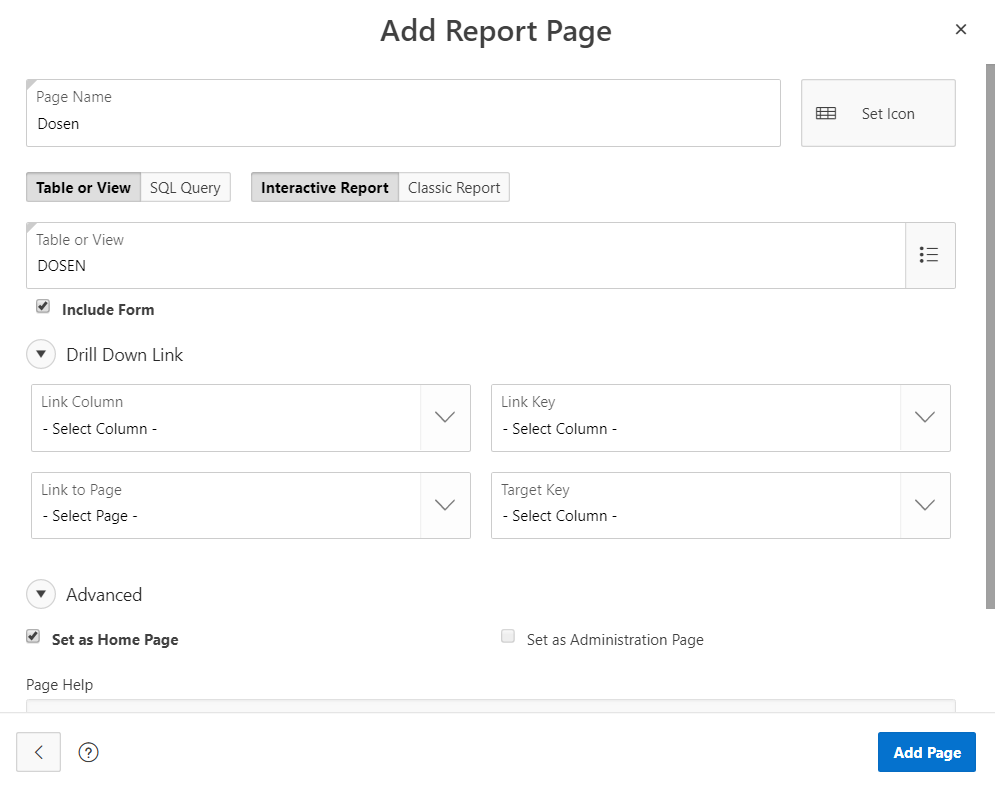
\includegraphics[width=8cm]{Figures/addpagedosen.PNG}}
        \end{figure}
    \item Lalu pilih add page kembali kemudian pilih interactive report. Isi table name sesuai urutan tabel, tabel nilai.
    \item Lalu pilih add page kembali kemudian pilih interactive report. Isi table name sesuai urutan tabel, tabel jadwal.
        \begin{figure}[h]
        \centerline{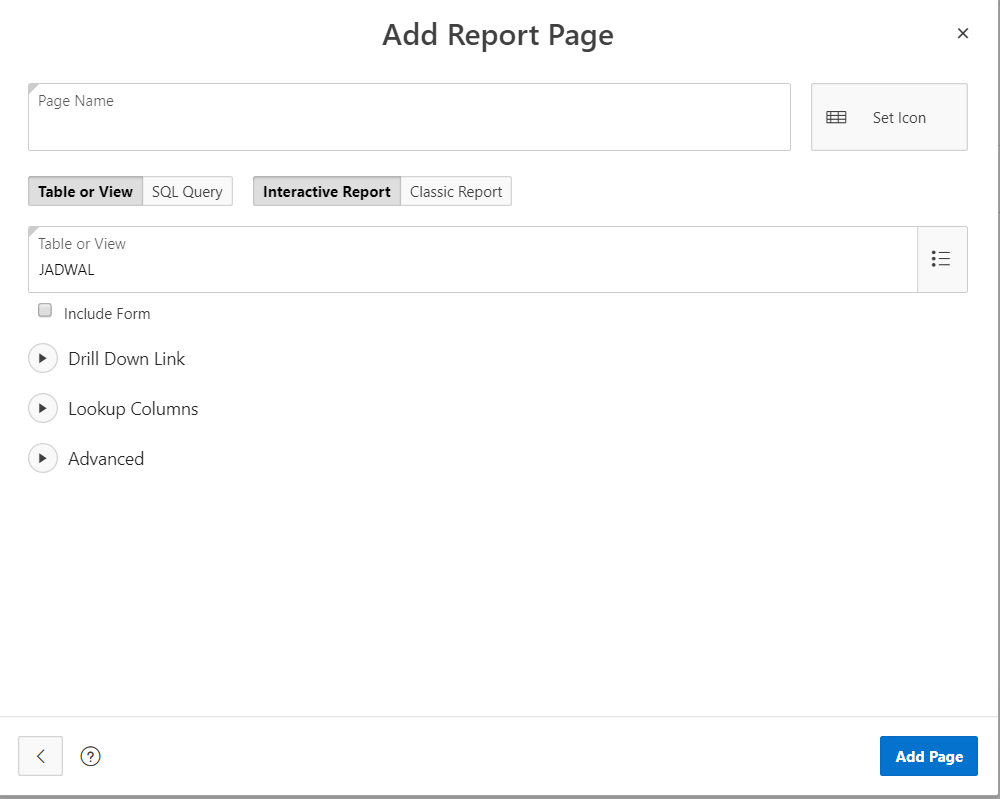
\includegraphics[width=8cm]{Figures/addpagejadwal.PNG}}
        \end{figure}
    \item Lalu create application
        \paragraph{}
        \centerline{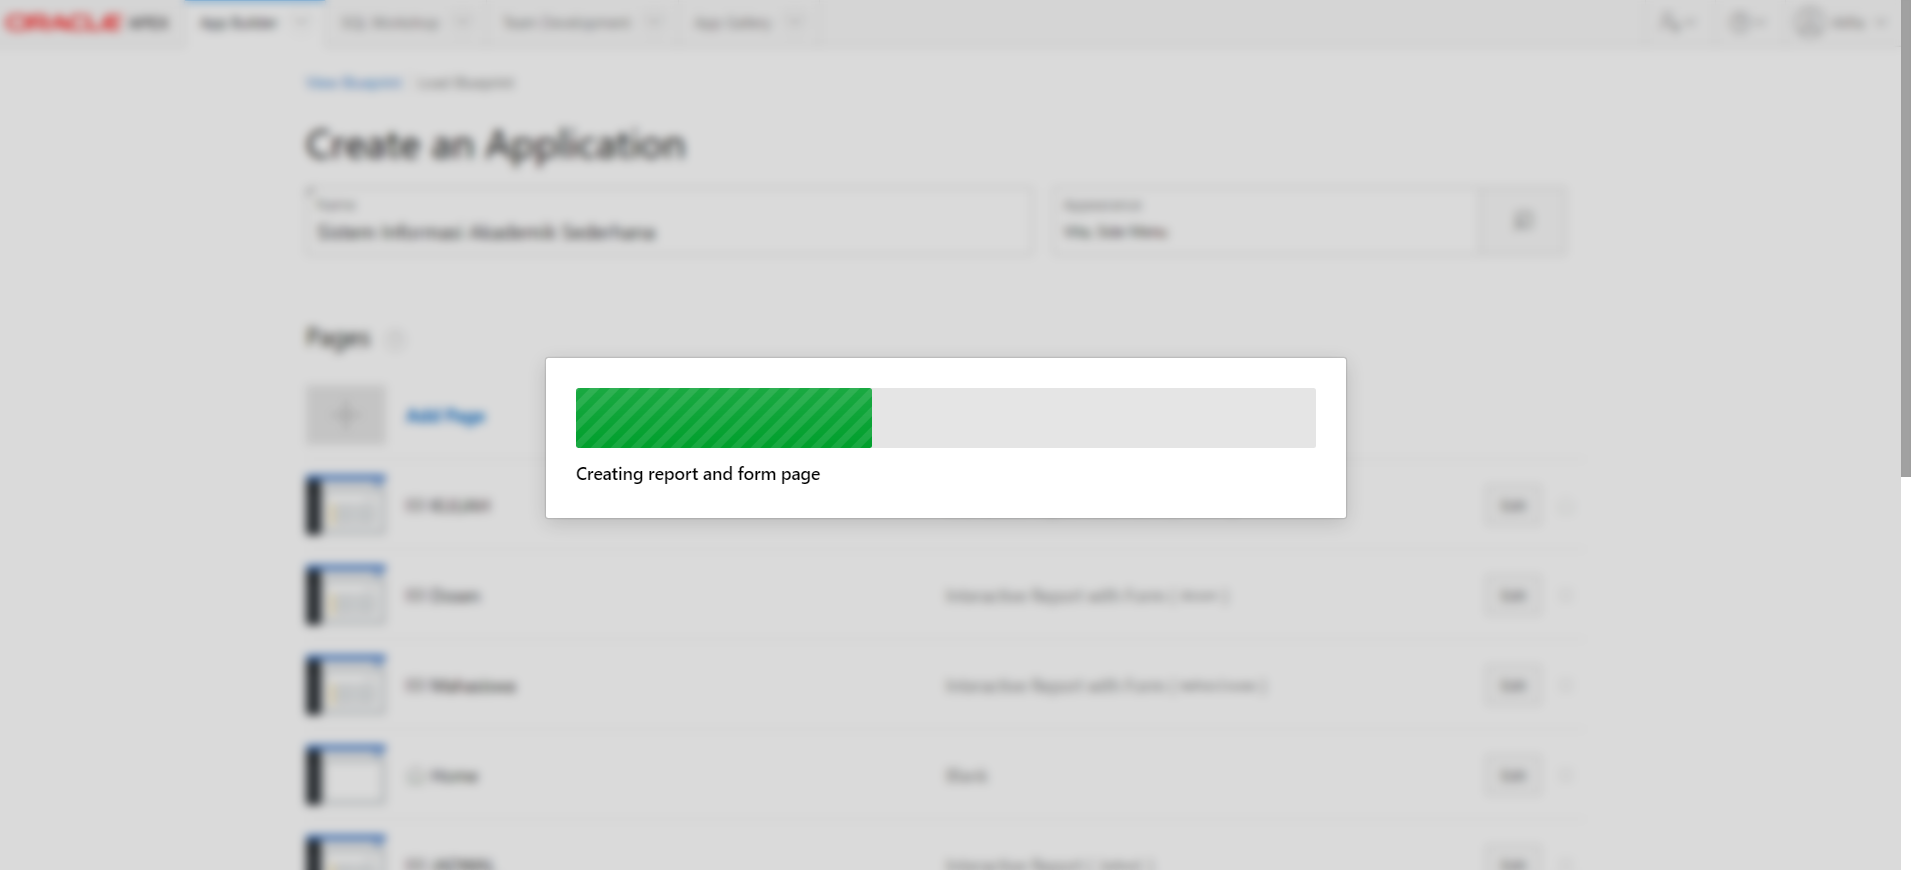
\includegraphics[width=8cm]{Figures/CREATE.PNG}}
    \item Lalu run application dan sign in kembali
    \item Selesai, aplikasi anda telah dibuat.
        \begin{figure}[h]
        \centerline{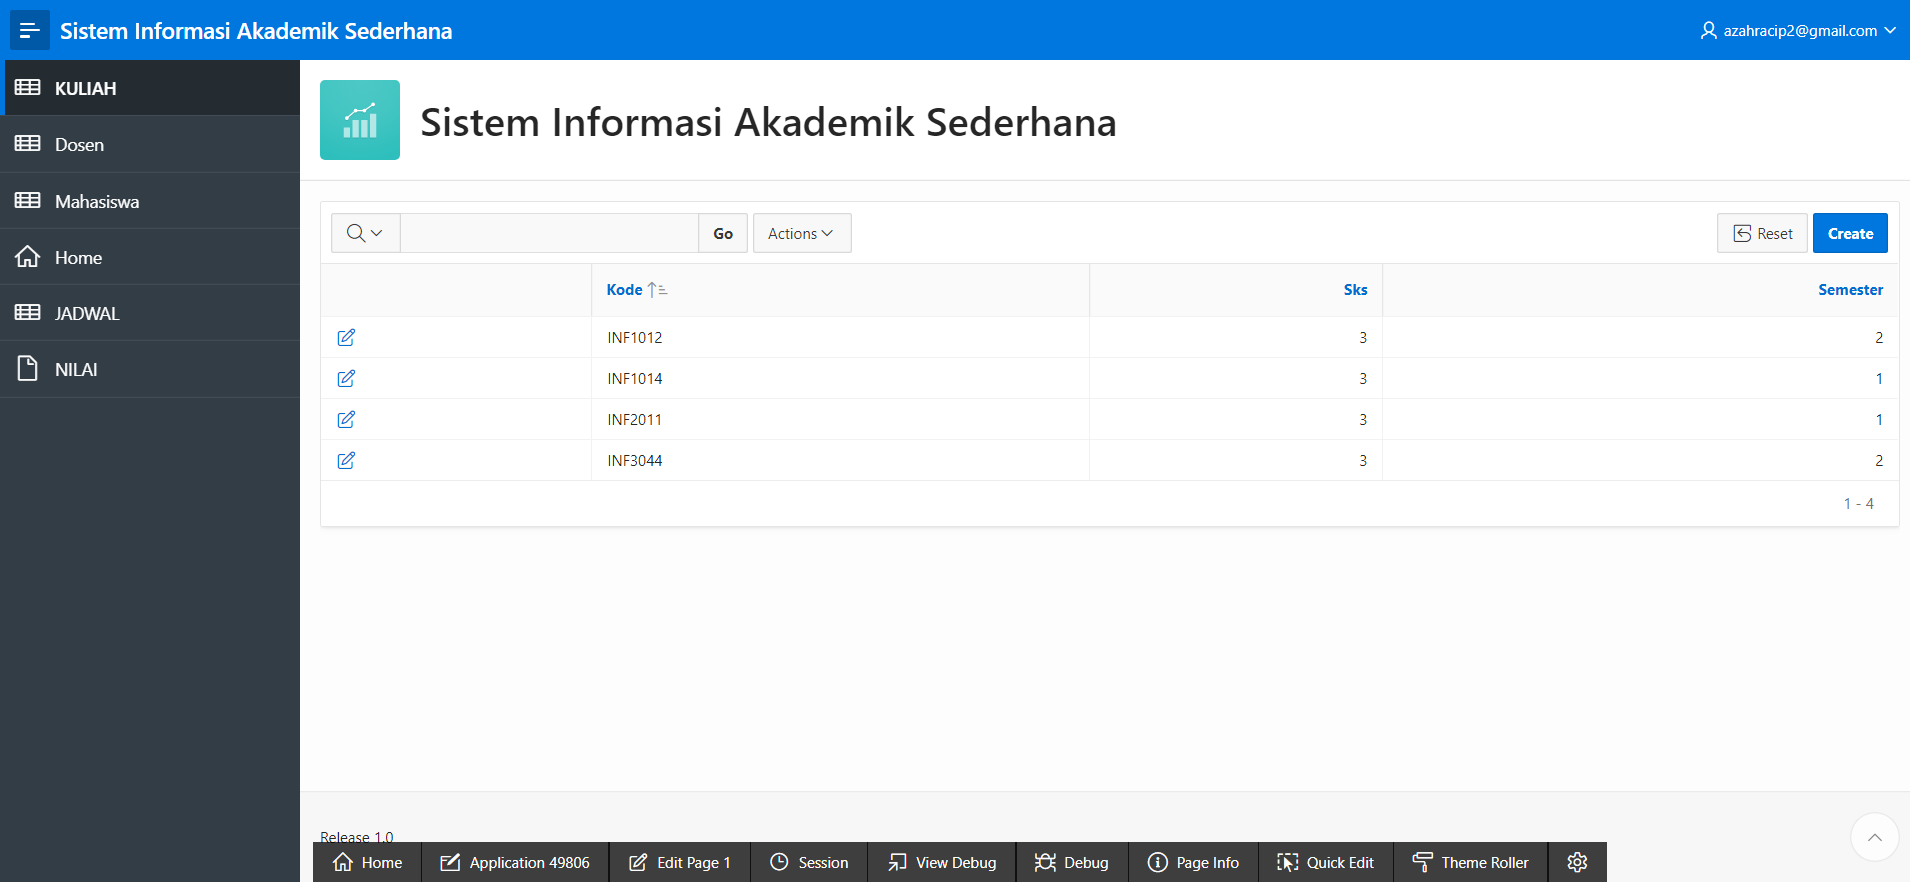
\includegraphics[width=8cm]{Figures/aplikasi.PNG}}
        \end{figure}
        
    \paragraph{}
    email/username : azahracip2@gmail.com
    \paragraph{}
    workspace : RARAALIFIA
    \paragraph{}
    password : 120201Ar
    
    
    
    
    
    
    
    
\end{enumerate}